%% cuthesis.tex
%% Minimal working example of Cardiff University,
%% School of Physics and Astronomy Thesis format
%% Copyright (C) Cardiff University 2012 --
%
% This work may be distributed and/or modified under the
% conditions of the LaTeX Project Public License, either version 1.3
% of this license or (at your option) any later version.
% The latest version of this license is in
%   http://www.latex-project.org/lppl.txt
% and version 1.3 or later is part of all distributions of LaTeX
% version 2005/12/01 or later.
%
% This work has the LPPL maintenance status `maintained'.
% 
% The Current Maintainer of this work is Duncan M. Macleod

\documentclass[11pt]{cuthesis}
\usepackage{graphicx}
\usepackage{setspace}
\setcounter{section}{-1}

\usepackage{rotating}
\usepackage{amsmath}
\usepackage{amssymb}
\usepackage{placeins}

\usepackage{appendix}
\usepackage{lscape} 
\usepackage{longtable}

\newcommand{\mn}{_{\mu\nu}}
\newcommand{\fs}{\text{ .}}
\newtheorem{theorem}{Theorem}[section]
\newcommand{\pd}{\partial}
\newcommand{\infint}{\int^\infty_{-\infty} }
\newcommand{\Fp}{F^{+}_{\alpha}}
\newcommand{\Fx}{F^{\times}_{\alpha}}
\newcommand{\tbd}{\tilde{\textbf{d}}}
\newcommand{\tbh}{\tilde{\textbf{h}}}
\newcommand{\xp}{X-pipeline }




% setup metadata
\title{Improved Methods for the Detection of Gravitational Waves associated with Gamma-Ray Bursts}
\author{Iain Dorrington}
\date{16th May 2019}

\usepackage{hyperref}

\begin{document}

% ----------------------------
% preamble

% print title page
\maketitle

% set preamble formatting
\frontmatter

% summary
\begin{abstract}
    I love hitting my head against a wall, so I did that for a bit.
\end{abstract}

% declaration - REQUIRED
\declaration

% contents
\tableofcontents
\listoffigures
\listoftables

% dedication
\begin{dedication}
    ``[T]he Listeners are trying to work out precisely what it was that the Creator said when He made the universe...  There were certain problems caused by the fact that they didn't hear only the subtle echoes of the first words, but every other sound made on the Disc. In order to recognise the sound of the Words, they had to learn to recognise all the other noises. This called for a certain talent, and a novice was only accepted for training if he could distinguish by sound alone, at a distance of a thousand yards, which side a dropped coin landed. He wasn't actually accepted into the order until he could tell what colour it was."\\
    \vspace{1cm}
    \hfill \textit{Terry Pratchett}
\end{dedication}

% ----------------------------
% main work

\mainmatter

\chapter{Introduction}
\begin{itemize}
\item Usual 'start of GW astronomy' stuff
\item LIGO interferometer stuff. Virgo too. Soon Kagra and LIGO India
\item GRBs are good candidate sources for GWs, especially after 170817A
\item Triggered vs untriggered search
\item There are several different search strategies for GRB GWs. They vary in the number of assumptions that they make about the source. This thesis covers two of these searches: The modelled CBC search, which assumes an inspiral, and the unmodelled Xpipeline search, which only a maximum duration and bandwidth of the GW.
\item PyGRB and X are both triggered searches
\item PyGRB assumptions are restrictive enough to allow a matched-filter search 
\item PyGRB can be made more sensitive by assuming circularly polarised GW emission, as the beam is perpendiular to the plane of the system
\item Indicate the median exlcusion distance for BNS systems or something like that to show how sensitive PyGRB is
\item Xpipeline is a GWB search that makes minimal assumptions
\item It only uses measures of coherence based on sky location
\item O2 median distances
\item Improved this search using machine learning
\item Describe format of thesis
\end{itemize}


\chapter{Gravitational Wave Astronomy in a Nutshell} \label{chap: gw bg}



\section{Gravitational waves}
General Relativity shows that spacetime can curve and move. From this, it may seem obvious that waves can travel though spacetime. But this is not a trivial fact; Einstein himself, having introduced the concept of gravitational waves in 1916, later claimed they could not exist. In this section, we will show that gravitational waves do exist. We will do this by considering a perturbation of the flat Minkowski metric. We will then calculate the Ricci tensor and Ricci scalar for the perturbed metric and, with a clever choice of gauge transformation, see that these yield a wave solution to Einstein's equations. 

\subsection{Linearised Gravity}
Let $g\mn$ be the metric given by adding a small perturbation $h_{\mu\nu}$ to the Minkowski metric $\eta\mn=\text{diag}(-1,1,1,1)$. We write this metric as 
\begin{equation} \label{pert metric}
g\mn=\eta_{\mu\nu}+h_{\mu\nu} \text{, } \hspace{20pt} |h_{\mu\nu}| \ll 1 \text{ .}
\end{equation}

To first order in $h$, we calculate the Ricci tensor (\ref{rt})
\begin{equation} \label{lin rt}
R\mn =\eta^{\alpha \beta}R_{\alpha \mu \beta \nu} = \frac{1}{2}\left( \pd_\mu \pd ^\alpha h_{\alpha \nu} + \pd_\nu \pd_\alpha h^\alpha_\mu -\Box h\mn -\pd_\mu \pd_\nu h \right)
\end{equation}
and the Ricci scalar (\ref{rs}) 
\begin{equation} \label{lin rs}
R=\eta^{\mu \nu}R\mn=\pd _\mu \pd_ \alpha h^{\mu \alpha} - \Box h \textbf{,}
\end{equation}
where $\Box=\pd_\mu \pd^\mu $ is the d'Alembertian operator and $h=h^\mu_\mu$ is the trace of $h$. From these, we find the resulting Einstein tensor is also linear in $h$ 
\begin{equation} \label{lin Einstein}
\begin{split}
G\mn & =R\mn -\frac{1}{2} R \eta\mn \\
 & = \frac{1}{2} ( \partial_\sigma \partial_\nu h^\sigma_\mu + \partial_\sigma \partial_\mu h^\sigma_\nu - \partial_\mu \partial_\nu h - \square h\mu -\eta\mn \partial_\rho \partial_\lambda h^{\rho \lambda} + \eta\mn \square h ) /fs
\end{split}
\end{equation}

\subsection{Gauge Transformation}
The metric given in \ref{pert metric} does not uniquely define a coordinate system, as there may be other coordinates where the metric is given by the Minkowski metric plus some other perturbation. This gives us the freedom to choose some coordinates that make the linear Einstein tensor simpler. To find these coordinates, we start with the following gauge transformation
\begin{equation}
x^{\mu'}=x^\mu +\chi ^\mu (x)\text{,} \hspace{20pt}\partial_\mu \chi^\nu \ll 1\fs
\end{equation} 
This gives us
\begin{equation}
\frac{\pd x^\mu}{\pd x^{\alpha'}}=\delta^\mu_\alpha-\pd_\alpha\chi^\mu +\mathcal{O}(|\pd \chi|^2) \fs
\end{equation}  
Applying these results to our metric (\ref{pert metric}) we find
\begin{equation} 
g_{\alpha' \beta'}=\frac{\pd x^\mu}{\pd x^{\alpha'}}\frac{\pd x^\nu}{\pd x^{\beta'}}g\mn=g_{\alpha \beta}-\pd_\alpha \chi_\beta -\pd_\beta \chi_\alpha \fs
\end{equation}
Subtracting the Minkowski metric from each side, we find 
\begin{equation} \label{pert transf}
h_{\alpha' \beta'}=h_{\alpha \beta}-\pd_\alpha\chi_\beta-\pd_\beta\chi_\alpha \fs
\end{equation}

We have some freedom in choosing our $\chi$, so we impose the \textit{harmonic gauge condition}
\begin{equation} \label{harmonic gauge}
\partial_\mu h^\mu_\nu = \frac{1}{2} \partial_\nu h \text{,}
\end{equation}
where $h=h^\lambda_\lambda$. We can always choose a $\chi$ such that this is true. To see this, first note that $\partial'_\mu = \partial_\mu - (\partial_\mu \chi^\lambda) \partial_\lambda$. From this we find
\begin{equation}
(\partial_\mu' {h'}_\nu^\mu - \frac{1}{2}\partial_\nu' h') \approx (\partial_\mu h^\mu_\nu - \frac{1}{2} \partial_\nu h ) -\square \chi_\nu \fs
\end{equation}
Thus, if we are given an $h$ such that \ref{harmonic gauge} is not true, we can choose a $\chi$ such that 
\begin{equation} \label{harmonic chi}
\square \chi_\nu = (\partial_\mu h^\mu_\nu - \frac{1}{2}\partial_\nu h) \fs
\end{equation}

Using \ref{harmonic gauge}, we can simplify the Ricci tensor and scalar
\begin{equation}
R\mn = -\frac{1}{2}\Box h\mn
\end{equation}
\begin{equation}
R=-\frac{1}{2}\Box h \fs
\end{equation}
Using these in the linearised Einstein equations (\ref{lin Einstein}) gives us
\begin{equation}
\Box h\mn - \frac{1}{2}\eta\mn\partial^2 h =-\frac{16\pi G}{c^4}T\mn \fs
\end{equation}
Alternatively, we can use \ref{alt einstein} to write this as
\begin{equation}
\Box h\mn = -16\pi G \left( T\mn -\frac{1}{2} \eta\mn T \right). 
\end{equation}
In a vacuum, the right hand side of this equation becomes zero, and we can recognise as the relativistic wave equation
 \begin{equation}
\Box h\mn = 0 \fs
\end{equation}

\subsection{Physical Effects of Gravitational Waves}
The plane wave solution for the vacuum wave equation is
\begin{equation} \label{plane wave}
h\mn (x) = \epsilon\mn e^{ik_\alpha x^\alpha} 
\end{equation}
where $\epsilon\mn$, the polarisation tensor for the gravitational wave, is symmetric and constant, and $k^\alpha$ is the 4-wave-vector given by $k^\alpha = (\omega,\vec{k})$. Subsituting this into the vacuum wave equation, we find 
\begin{equation}
k_\alpha k^\alpha = -\omega^2 + |\vec{k}|^2 =0 \fs
\end{equation}
Hence, gravitational waves travel at the speed of light. 

The polarisation tensor must satisfy the wave equation and the harmonic gauge condition. Putting the wave solution \ref{plane wave} into the harmonic gauge condition \ref{harmonic gauge}, we find that gravitational waves are transverse

\begin{equation}  \label{harmonic gauge2}
k_\mu \epsilon^\mu_\nu = \frac{1}{2}\partial_\nu \epsilon
\end{equation}
where $\epsilon=\epsilon^\lambda_\lambda$.

We can impose further gauge conditions as long as the harmonic gauge (and hence \ref{harmonic gauge2}) is not violated. As any transformation with $\square \chi = 0$ will satisfy \ref{harmonic chi}, and hence harmonic gauge condition, we express $\chi$ as 
\begin{equation} \label{chi form}
\chi_\nu = X_\nu e^{ikx} \fs
\end{equation}
Using \ref{chi form} and \ref{plane wave} in the transformation equation \ref{pert transf}, we find the transformation equation for the polarisation tensor
\begin{equation} \label{epsilon tranform}
\epsilon'\mn = \epsilon\mn -ik_\mu X_\nu - ik_\nu X_\mu \fs
\end{equation}
Taking the trace of this, we find
\begin{equation}
\epsilon'^\mu_\mu = \epsilon^\mu_\mu - 2ik^\mu X_\mu \fs
\end{equation}
Thus, we can impose the further gauge condition that the polarisation matrix be traceless by choosing coordinates such that $2ik^\mu X_0 = \epsilon^\mu_\mu - 2ik^i X_i$. Using this in \ref{harmonic gauge2}, we find
\begin{equation} \label{harmonic gauge 3}
k^\mu \epsilon\mn = 0 \fs
\end{equation}
We can fix the other elements of $X_\mu$ by setting $\epsilon_{i 0} = 0$ for $i=1,2,3$. We do this using \ref{epsilon tranform} to find
\begin{equation} \label{epsilon 0}
\epsilon'_{i 0} = \epsilon_{i 0} -ik_i X_0 - ik_0 X_i \fs
\end{equation}
Now we see that by choosing the $X_i$ such that $ ik_0 X_i = ik_i X_0 - \epsilon_{i 0}$, we have $\epsilon'_{i 0} = 0$. The gauge defined by the above conditions is called the \textit{transverse-traceless} (TT) gauge.

%These conditions give us that $\epsilon_{0 0} = 0$ as well. Using the fact that the polarisation matrix can be assumed traceless $\epsilon^\mu_\mu$, the wave solution \ref{plane wave} reduces the harmonic gauge condition \ref{harmonic gauge} to 
%\begin{equation}
%\partial_\mu h^\mu_\nu = 0 \fs
%\end{equation}
%As $\epsilon_{i 0} = 0$, in the $\nu = 0$ case, only the $\mu=0$ term is non-zero. Thus we are left with
%\begin{equation}
%\partial_\mu h^\mu_0 = \epsilon^0_0 i k_0 e^{ik_\alpha x^\alpha} = 0 \fs
%\end{equation}
%Which implies $\epsilon^0_0=0$. As the polarisaton tensor is symmetric, we have $\epsilon^3_3=0$ as well.  

To make things even simpler, assume the wave is traveling in the z-direction, that is $\vec{k} = (0,0,\omega)$. The transverse condition \ref{harmonic gauge 3} gives us $\epsilon_{0\nu} = \epsilon_{3\nu}$. This gives us $\epsilon_{0 0}= 0$ and $\epsilon_{3 i} = 0$, as we already have $\epsilon_{3 0}$. The traceless condition then becomes $\epsilon_{1 1} + \epsilon_{2 2} = 0$. Using the symmetry of the polarisation matrix to fill in the rest of the matrix, we find the following solution to \ref{plane wave} 
\[
h\mn (x)
=
\begin{bmatrix}
0 & 0 & 0 & 0 \\
0 & \epsilon_+ & \epsilon_\times & 0 \\
0 & \epsilon_\times & -\epsilon_+ & 0 \\
0 & 0 & 0 & 0 
\end{bmatrix}
e^{(i\omega (z-t))} \fs
\] 
We can see that the polarisation matrix is fully described by two real numbers $\epsilon_+$ and $\epsilon_\times$. We call these the plus and cross polarisation of the gravitational wave.


\section{Gravitational Waves Sources} 
\begin{itemize}
\item GW generation 
\item Sources
\begin{itemize}
\item BBH - Multiple found already
\item BNS - One found and Hulse-Taylor
\item NSBH
\item GRB 
\item SN
\item Unknown
\end{itemize}
\end{itemize}
\section{Gravitational Wave Detectors} \label{sec:gw detectors}
Can cite soaulson and the noises paper
\begin{itemize}
\item Michelson Interferometer (cite R.Weiss 1972 paper to look smart)
\item Measure change in output power due to interference in the arms
\item Noise sources and how they are mitigated
\begin{itemize}
\item Autocorrelation function
\item PSD and ASD (tie back to the noise budget) 
\item Fundamental noise
\item Environmental noise
\item Instrumental noise
\item Noise budget
\end{itemize}
\item Detector nulls
\end{itemize}


\begin{figure} % Example of including images
\begin{center}
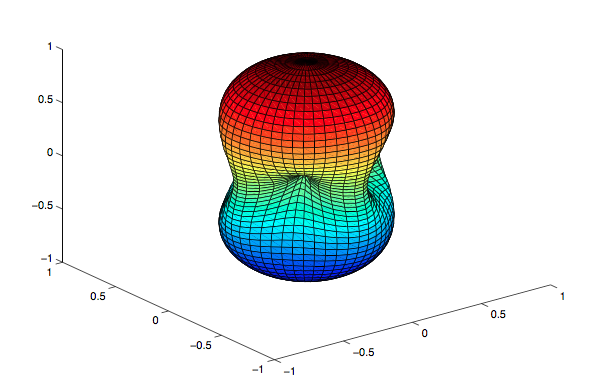
\includegraphics[width=0.8\linewidth]{antenna_pattern.png}
\end{center}
\caption{\textbf{Antenna Pattern.} \textbf{cite Sathya and Schutz living review} }
\label{fig:antenna pattern}
\end{figure}


\chapter{Gamma-Ray Bursts} \label{chap:GRBs}
\textit{Gamma-ray Bursts} (GRBs) are exceptionally energetic flashes of gamma rays. They can last from just a few milliseconds up to several hours and have highly variable luminosity curves (see figure \ref{fig:grb lightcurves}). They are detected at a rate of about one per day, are uniformly distributed over the sky, and are the most electromagnetically energetic objects in the universe. The short duration and huge energy emitted by GRBs suggests a violent origin, making them strong candidates for gravitational wave (GW) emission.

In this chapter we discuss GRB astrophysics. We will begin with some historical perspective, starting with the accidental first detection of a GRB in 1963 and continuing to the first GW detection associated with a GRB in 2017. We will see that GRBs can be classified as short-hard or long-soft, depending on their duration and spectral hardness. We will see the evidence that long GRBs are caused by core collapse supernova, and that short GRBs are caused by compact binary mergers involving at least one neutron star. We will discuss the physical processes that could be powering GRBs and what GW astronomy can teach us about these processes. We end this chapter with a discussion of current GRB detectors and search strategies for GW emission associated with GRBs.

\begin{figure} % Example of including images
\begin{center}
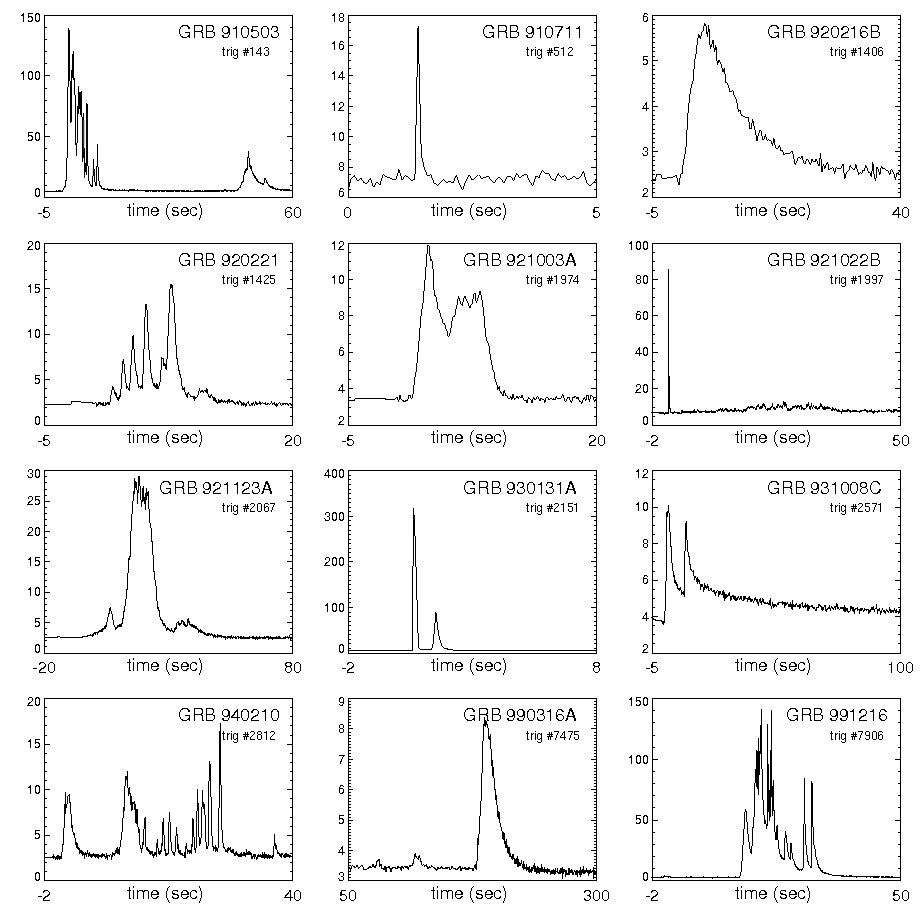
\includegraphics[width=1.0\linewidth]{grb_lightcurves.png}
\end{center}
\caption{\textbf{BATSE gamma-ray light curves.}  \textbf{cite http://inspirehep.net/record/1358907/plots} }
\label{fig:grb lightcurves}
\end{figure}

\section{The History of Gamma-ray Burst Astronomy} \label{sec:GRB history}
In this section we will discuss the key discoveries of GRB astronomy in their historical context. These discoveries are the motivation of GW searches associated with GRBs, and were used to develop the GW searches discussed in chapters \ref{chap: CBC} and \ref{chap: mva}.  

\subsection{Cold War Tension and an Unexpected Discovery} \label{sec:cold war}
The partial nuclear test ban treaty, agreed between the USA and the Soviet Union in 1963, banned atmospheric, underwater, and outer space nuclear weapon tests. This created a technical challenge: how to enforce the ban? Seismic sensors could be used for on-Earth tests, but would not work for outer space tests. The solution was to look for the flash of gamma-rays produced in the first milliseconds of a nuclear explosion. Thus the Vela and Kosmos gamma ray detecting satellites were produced by the USA and Soviet Union respectively. These satellites contained only rudimentary gamma ray detectors, and each individual satellite was not capable of localisation. Some localisation was possible using time delay and Earth blocking information.

These satellites started to detect brief bursts of gamma rays, which were first reported in 1973. These events did not look like those expected from a nuclear test, and did not seem to be coming from the Earth or any nearby astronomical bodies such as the moon. It appeared a new, high-energy astronomical phenomenon had been discovered. 

This phenomena, called \textit{Gamma-ray Bursts} (GRBs), would appear and fade away in as little as a milliseconds, and could be as brighter than the rest of the gamma ray sky combined. The brevity of these events placed constraints on the size of the source, as the crossing time for a region cannot be less than the light travel time. Thus a 1ms GRB must have a source smaller than 300km across. This limits the potential candidates down to compact objects, such as neutron stars and black holes, or to small regions of larger objects, such as the cores of massive stars. Another important feature of GRBs is that the bursts do not repeat. This suggests a source that is destroyed when the GRB is produced. More measurements were needed to narrow down the number of possible sources for GRBs. 

\subsection{BATSE and the Galactic/Extra-galactic Controversy}
Most early GRB detectors could not localise well. It was known that GRBs were not coming from any planets in the solar system or from the galactic center, but otherwise the location of GRB sources was a mystery. In particular, it was not clear whether GRBs were coming from galactic or extra-galactic sources. Answering this question was an important step towards identifying the origin of GRBs, as an extra-galactic source would require far greater energy than a galactic source to produce a GRB of equal brightness. 

Better sky localisation would help to answer this question. If GRBs mostly occur on the galactic plane, then they are probably of galactic origin. If they were clustered around nearby galaxies, then GRBs probably come from those galaxies. If, however, they are distributed isotropically on the sky, then it would be likely that GRBs form at cosmological distances.\footnote{It should be noted that there are other ways that GRBs could be isotropically distributed. If they are only detectable to a few hundred parsecs, they would be entirely within the disc of the galactic plane and so would also be isotropically distributed. Alternatively, as neutron stars receive a `kick' during their formation, they could form a corona around the galaxy.}

Improved sky localisation was achieved in 1991, with the launch of the Burst and Transient Source Experiment (BATSE) on the Compton Gamma-ray Observatory. With BASTSE, it became possible to determine the sky position of a GRB to within half a degree. During its mission, BATSE detected approximately 2700 GRBs and determined the sky position of a large number of these. For the first time their was a statistically significant sample of well localised GRBs. In figure \ref{fig:batse grb fluence} we can see the sky location of every GRB detected by BATSE, together with the fluence\footnote{Fluence is the time integral of the flux. Essentially a measure of the total detected energy.} of that GRB. This plot shows that GRBs are isotropically distributed over the sky. This evidence strongly suggests GRBs are of cosmological origin. 


\begin{figure} % Example of including images
\begin{center}
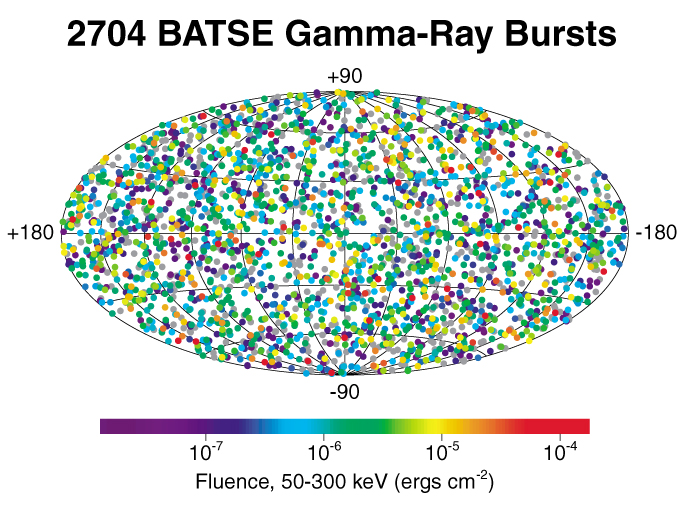
\includegraphics[width=0.8\linewidth]{batse_grbs_fluence.jpg}
\end{center}
\caption{\textbf{BATSE GRB Fluence.} This plot shows the fluence (given by the colour of each point) and the sky position of each GRB detected by the BATSE mission. \textbf{cite \url{https://heasarc.gsfc.nasa.gov/docs/cgro/images/cgro/2704_grbs_fluence.jpg}}}
\label{fig:batse grb fluence}
\end{figure}

The BATSE data also provided evidence that GRBs were uniformly distributed and that we were seeing a limited horizon, beyond which GRBs became much harder to detect. This evidence came in the form of a $\log N - \log P$ distribution, where $N$ is the number of detected GRBs and $P$ is the peak flux\footnote{Some times the $\log N - \log S$ distribution is preferred, with $S$ being the given flux. The essence of the plots is the same.}. If GRBs are uniformly distributed in space then the number of GRBs out to a given distance increases as the cube of that distance. However, peak flux from the GRBs would decrease with the inverse square of the distance. Hence, plotting  $\log N$ against $\log P$, we expect to find a gradient of approximately $-3/2$. Any short fall from this expected distribution suggests that we have reached a horizon for detectable GRBs. In figure \ref{fig:logn - logp} we see the $\log N - \log P$ distribution for a combined set of GRBs detected by BATSE and the Pioneer Venus Orbiter (PVO).\footnote{ The PVO was less sensitive than BATSE, but it operated for 10 years and so observed a fairly large number of GRBs}. The gradient for high energy GRBs is the expected $-3/2$ but there is a shortfall at low energies, suggesting there is a limited distance to which GRBs can be viewed. Unfortunately this data does not inform us of where that horizon is. It could be within our galaxy, or it could be the horizon of the universe.   


\begin{figure} % Example of including images
\begin{center}
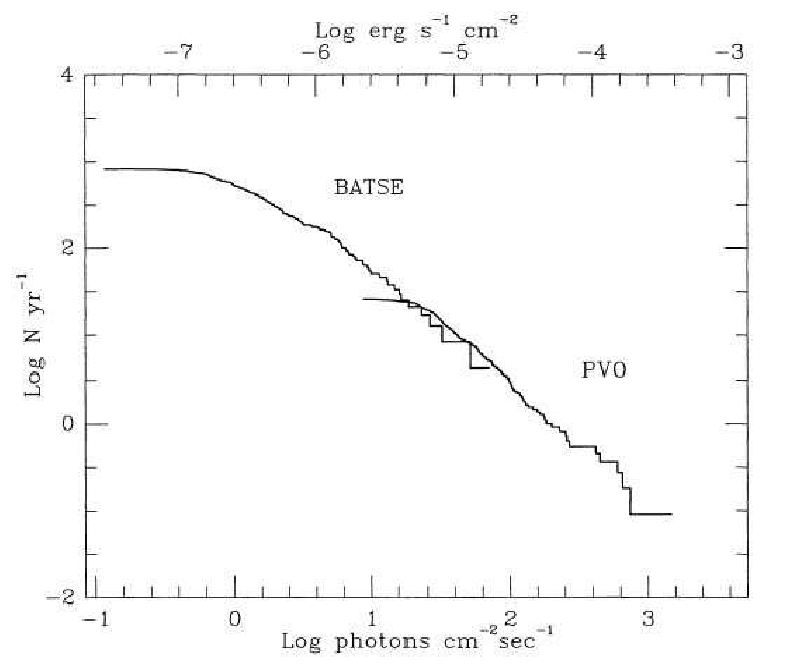
\includegraphics[width=0.8\linewidth]{logN-logP.png}
\end{center}
\caption{\textbf{LogN-logP for BATSEVPO.} Here we plot the log of the number of GRBs against the log of the peak flux. The sample includes GRBs detected by BATSE and by PVO. The energy range for BATSE was 50-300keV, and the energy range for PVO was 100-2000keV. For uniformly distributed GRBs, we expect this plot to have a gradient of $-3/2$. The expected gradient is observed for high energy GRBs but not at lower energies. This suggests a limited distance to which GRBs can be observed. 
\textbf{cite \url{https://www.researchgate.net/figure/Distribution-log-N-log-P-for-a-combined-set-of-BATSEPVO-data-The-distributions-match_fig5_242389649}}
\textbf{cite \url{https://www.nature.com/articles/366040a0.pdf}}
}
\label{fig:logn - logp}
\end{figure}

\subsection{The Long and Short of Gamma-ray Bursts}
Another important piece of evidence into the origins of GRBs came from their duration. As every burst has different properties\footnote{For example, some bursts have multiple flares.} the duration of a GRB is not trivially defined. The measure most commonly used is the $T_{90}$, the time over which $90\%$ of the total fluence is recorded.\footnote{Another common measure is the similarly defined $T_{50}$.} 

The top panel of figure \ref{fig:t90 vs hardness} shows the number of bursts with a given $T_{90}$ for the BATSE data. This plot shows that there are two populations of GRBs, the first with a $T_{90}$ value of about 0.5s and the second with a $T_{90}$ of about 30s. It is also clear from this data that the longer population of GRBs are detected far more often. Plotting the spectral hardness of the BATSE GRBs against $T_{90}$, as has been done if figure \ref{fig:t90 vs hardness}, we see that the shorter GRBs also have a harder spectrum than the longer GRBs. This means short GRBs emit more high energy photons than long GRBs. Because of these two properties of the two populations, they are known as \textit{short-hard} and \textit{long-soft} GRBs. It is common to use the criteria that short GRBs are those that are less than 2s, and long GRBs are longer than 4s, with those inbetween being called \textit{intermediate} GRBs.

%\begin{figure} % Example of including images
%\begin{center}
%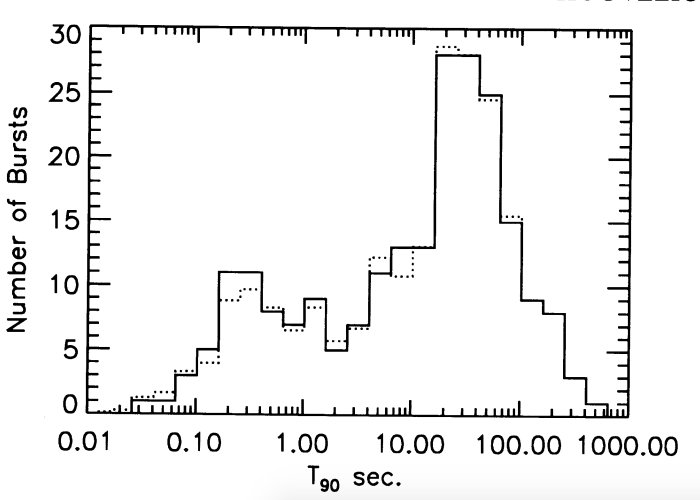
\includegraphics[width=0.8\linewidth]{t90_vs_count.png}
%\end{center}
%\caption{\textbf{T90 vs count.} Here we plot the $T_{90}$ values against the the count of GRBs for the BATSE mission as of 1993. \textbf{cite identification of two classes of gamma ray bursts} \textbf{what is the difference between the dotted line and the solid line-read original paper.}}
%\label{fig:t90 vs count}
%\end{figure}

It should be mentioned that while $T_{90}$ is a very useful tool, it is instrument dependent. This is because more sensitive instruments will track GRBs for longer, and bursts have different durations in different energy bands. Also, the $T_{90}$ is measured in the detector frame, and not the rest frame of the burst, which would make a GRB at a redshift of $z$ appear a factor of $(1+z)$ longer. For these reasons, using the $T_{90}$ to classify short/long GRBs should only be considered approximate.  

As a final note on GRB durations, it should be mentioned that there is some evidence that there may be intermediate and ultra-long populations of GRBs. It is an open question whether these GRBs represent new populations of GRBs or are part of the long and short GRB populations. As these are still contentious, we do not consider them further. 




\begin{figure} % Example of including images
\begin{center}
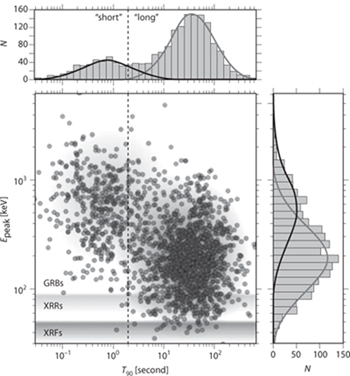
\includegraphics[width=0.8\linewidth]{t90_vs_hardness_new.jpg}
\end{center}
\caption{\textbf{T90 vs the spectral hardness ratio.} Here we plot the $T_{90}$ values and the spectral hardness ratio for the BATSE GRBs. The top panel shows a histogram of the T90 data, which clearly has two populations of GRBs, short and long. The main plot shows T90 against spectral hardness, which makes the two populations even more clear and shows that short GRBs have harder spectra than long GRBs. Those GRBs with the greatest ratio of energy in the X-ray to gamma ray band, generally those with a peak energy of less than 15 keV, are called \textit{X-ray flashes} (XRF). Those with comparable energy in the gamma-ray and X-ray band are called \textit{X-ray rich} (XRR) GRBs. All other GRBs are simply called GRBs. These different classes of GRBs are marked on the plot. Also shown is the 2 second dividing line between short and long GRBs.  \textbf{cite What are Gamma-ray Bursts? Joshua Bloom}}
\label{fig:t90 vs hardness}
\end{figure}

\subsection{BeppoSAX and the First Afterglows}
Important clues had been found into the origin of GRBs, but still no one had found any trace of a GRB after the prompt emission (the initial flash of gamma-rays). The search area provided by GRB detectors at the time were too large for ground based telescopes to have a realistic chance of finding the source of the GRB, though attempts were made. This changed with the launch of the BeppoSAX satellite in 1996. BeppoSAX was able to localise to within a few arcminutes, much better than the half a degree BATSE was capable of.\footnote{It is true that the InterPlanetary Network, a network of GRB detectors placed on various spacecraft throughout the solar system (see section \ref{sec:grb detectors}), could localise better than BATSE. The problem was that it took too long find the sky position of the GRB using this method, and any trace of the GRB had disappeared before astronomers could find it.} It also had a Narrow-Field x-ray Instrument (NFI) to search for X-ray counterparts to GRBs.

On February 28th 1997 a GRB was detected by BeppoSAX that was localised well enough for the satellite to aim the NFI at it. A new X-ray source was detected that faded away slowly over the next few days. The lower energy emission detectable in the days after the prompt emission is called the GRB \textit{afterglow}, and this was what BeppoSAX had detected. The localisation was accurate enough to allow ground based telescopes to find the optical counterpart to this GRB as well. The optical images showed what some argued was a distant galaxy and others argued was a galactic nebula. On May 8th 1997, a GRB was detected by BeppoSAX and an optical counterpart quickly found. A spectrum was obtained for the counterpart which showed iron and magnesium absorption lines that had been significantly red-shifted. This showed that the GRB must have occurred at a distance greater than 5 Gpc and that the light passed through some gaseous cloud in a distant galaxy on its way to Earth. With this observation there could be no doubt that GRBs were originating at cosmological distances, as had been suspected.  

\subsection{The Fireball Model} \label{sec: fireball}
The \textit{fireball shock model} was developed in the 1990s. It attempted to describe the physical processes that cause GRBs without making many assumptions about the source of energy for the GRB, the \textit{central engine}. At this time the evidence was building that GRBs originated at cosmological distances. At such great distances the inferred energy emitted at the source is far higher, as much as a solar mass if emitted isotropically. Light-travel time arguments showed that GRB sources must also be small, at most hundreds of kilometers across (see section \ref{sec:cold war}). Realising that all GRBs are small and highly energetic was the starting point of the fireball shock model.

The next step was to notice that photons detected from GRBs are often above the pair production threshold\footnote{Although for GRB 170717A, this was not case. See section \ref{sec:gw170817} for more details} ($2\times m_e c^2\approx 1$MeV), and so should have created electron-positron pairs rather than gamma-rays. This problem is solved by assuming that the energy released drives a relativistic expansion from the source. In this case the energy of the photons in their rest frame is inversely proportional to the bulk Lorentz factor of the outflow, i.e. the energy in the rest frame of the photons is much lower. It also causes photons to bunch up just ahead of the relativistic matter that is emitting the photons, causing it to seem more energetic to an observer. Accounting for these factors, it can be shown that the Lorentz factor must be in the hundreds for a typical GRB. This is as compared to a Lorentz factor of approximately 1.001 for a fast supernovae, and corresponds to GRB velocities of at least 99.9\% of the speed of light. 

Combining the evidence for the high speed of the ejected matter with the small size of the emitting object means that a large amount of energy must be rapidly dumped into a small volume before the GRB is emitted. Most of the energy is in the form of photons, so this is called the \textit{radiation dominated} phase. This soup of photons with a small amount of matter is called the \textit{fireball}. The fireball expands and the Lorentz factor grows with it. As it expands, the energy is absorbed by the matter (protons and electrons) in the form of kinetic energy. This is the \textit{matter dominated} phase. Most of the particles are moving in the same direction now, with little random motion, i.e. the fireball has become cold. 

A mechanism is needed to turn this kinetic energy into a GRB. The simplest way to do this is to have the matter collide with slower moving matter surrounding the system. The matter is too sparse for direct collisions to happen enough to form a GRB. Instead, it is thought that magnetic fields near the edge of the fireball can cause the matter to slow down and radiate its energy. When the fireball interacts with the surrounding matter, the rapid change in temperature, pressure, and density travel through the medium faster than the medium can react. Like the sonic boom of a supersonic jet, this causes \textit{shocks} in the surrounding medium. It is these shocks that are thought to be the source of the GRB. Precisely how these shocks power a GRB is not known. \textit{Fermi acceleration} possibly plays a role. This is where charged electrons enter the shock and are reflected back by magnetic fields, increasing their kinetic energy. After several iterations of this, the electron can travel even faster than the shock. The magnetic fields could then cause the electrons path to curve, causing them to emit energy as synchotron radiation. Alternatively they might interact with photons, imparting their considerable energy onto the photon to create a high energy gamma-ray. This process is called \textit{inverse Compton scattering}. There is still a lot to learn about the processes that power the GRB.

There are also two hypotheses as to what the slower moving matter that the fireball collides with could be. The first is simply material around the star, the \textit{circumburst medium} (CBM). This is called an \textit{external shock scenario}. The other theory is that multiple shells of material are emitted, and the shocks are created when faster moving shells catch up with slower moving shells. This is called the \textit{internal shock scenario}. The internal shock method is generally favoured for the prompt emission. This is because GRB light curves are highly variable, with some showing multiple peaks (see figure \ref{fig:grb lightcurves}). This is easily explained by the multiple shocks of the internal shock scenario, but more difficult to explain for external shocks. External shocks are thought to be the cause of the GRB afterglow.



\subsection{Jets} \label{sec:jets}
The well-founded assumptions made by the fireball model, that GRB progenitors are small and dense, naturally lead to the prime suspects for powering GRBs being compact objects, such as black holes and neutron stars. If we assume that compact objects do play a role in generating GRBs, then it is not much of a jump to think that GRBs may be jetted. Jets are ubiquitous with both black holes and neutron stars: supermassive black holes and solar mass black holes have been observed to have jets, and highly magnetised, rotating neutron stars, called \textit{pulsars}, are also known to produce jets. Assuming that GRBs are jetted substantially lowers the inferred energy emitted by the source, which has implications for the physical mechanism that causes GRBs. It is therefore important to determine whether GRBs are jetted or not. 

What would be the observable effects of GRB jetting? The fireball model suggests that the ejected matter will have a very high Lorentz factor. Special relativity tells us that objects moving with high Lorentz factor $\Gamma$ emit most of their energy within an angle $\theta\approx 2/\Gamma$ radians of the direction of travel. This is called \textit{relativistic beaming}. If the matter is jetted and the beamed angle $\theta$ is less than the opening angle of the jet, then there will be no observable difference between isotropic emission and jetted emission, as the edge of the jet is not visible. However, once the matter reaches the interstellar medium it will begin to slow down, reducing the amount of beaming and increasing the angle to which the matter can be observed. Once the beaming angle has increased to a point where the edge of the jet is visible, the amount of energy being radiated towards the observer will suddenly drop, and this will happen across the electromagnetic spectrum at the same time. This \textit{break} in the spectrum is observable in the afterglow of many GRBs. For example, figure \ref{fig:jetbreak} shows the clearly visible break in the afterglow spectrum of GRB 990510 after approximately one day. It is now widely accepted that short GRBs have opening angles of $\sim 30^\circ$ and long GRBs have opening angles of $\sim 5^\circ$.

\begin{figure} % Example of including images
\begin{center}
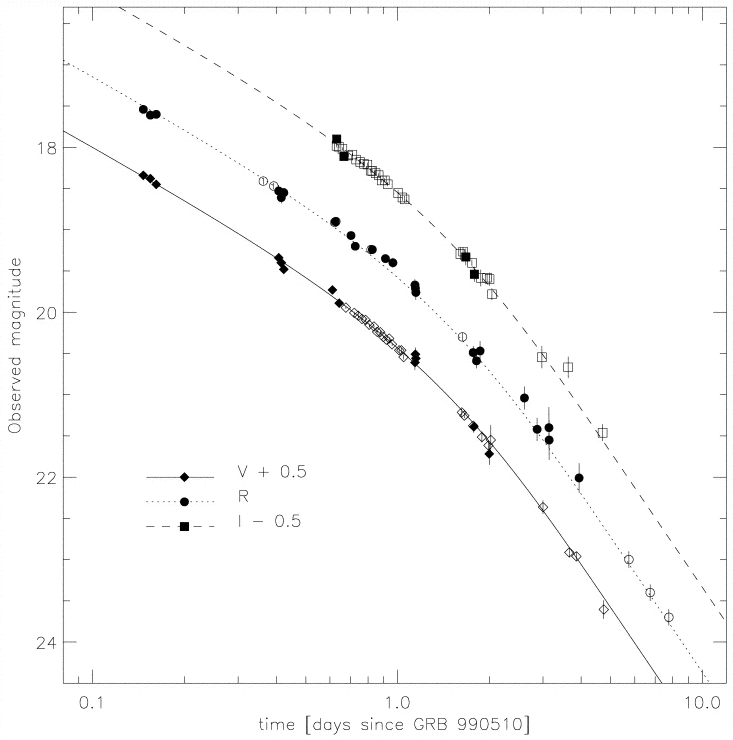
\includegraphics[width=0.8\linewidth]{jetbreak.png}
\end{center}
\caption{\textbf{Break in spectrum due to jetting.} Here we see the optical light curves for the afterglow GRB 990510. A break in the spectrum is visible after approximately one day. \textbf{cite \url{https://iopscience.iop.org/article/10.1086/312282/fulltext/} }}
\label{fig:jetbreak}
\end{figure}

\subsection{The Long GRB-Supernova Connection}
As more afterglows were found, trends began to appear. Long GRBs tended to occur directly on host galaxies, not randomly in space.\footnote{We will see in section \ref{sec: short grbs} that this is unlike short GRBs. which can originate quite far from any host galaxy.} Spectroscopy of these galaxies often found the presence of emission lines excited by star formation. In fact, no long GRB has been found in a non-starforming galaxy. The host galaxies also tended to be relatively faint. Low luminosity (i.e. low stellar mass) suggests galaxies have a low metallicity [\textbf{cite someone}], and spectographic studies confirmed this. Star forming galaxies with low metallicity, such as those from which long GRBs originate, are also where type 1b and 1c supernovae are observed. Type 1b and 1c supernovae result from the core collapse of massive stars that have shed off their outer layers of hydrogen. In the case of type 1c supernovae, they have also shed most or all of their helium as well. That long GRBs originate from star forming galaxies with low metallicity raises the possibility that long GRBs are connected to the massive stars that can only exist in these kinds of galaxies. In particular, it is thought that a type 1b or 1c supernova could power a GRB.

The strongest evidence of a supernova connection came with the detection of GRB 980425. This GRB was exceptionally close; at just $z=0.0085$ it is still the closest GRB ever detected. Followup observations found a rising supernova, SN 1998bw. It was a very bright supernova, about ten times brighter than normal. It also showed no hydrogen or helium emission lines, making this a type 1c supernova. It seemed highly unlikely that the coincident GRB and supernova were unrelated. Questions remained though, because this GRB was exceptionally faint given its distance. Was it typical of other long GRBs? 

After GRB 980425, searches were undertaken for other bright supernova afterglows associated with long GRBs. Not only were many found, but they were shown to have similar spectra to GRB 980425. In particular, GRB 030329 was another nearby GRB, at redshift $z=0.17$, which had very detailed followup. It was 1000 times brighter than GRB 980425, but showed the same spectral features. With this discovery, the consensus grew that long GRBs were caused by type Ic supernova.


\subsection{The Short GRB-Compact Binary Connection} \label{sec: short grbs}
Much had been learned about long GRBs by studying their afterglows, but no afterglow had been found for short GRBs. This was because short GRBs fade rapidly, reducing the amount of time for follow up observations. Rapid follow up was needed, and so the \textit{Swift} satellite (see section \ref{sec:grb detectors}) was launched in 2004. Swift was able to autonomously followup a GRB with X-ray, UV, and optical measurements within minutes, just what was needed for short GRBs. 

The first detected short GRB afterglow was that of GRB 050509B. It was a faint X-ray afterglow that faded quickly, but it was localised well enough for ground based telescopes to determine the host galaxy, which had a redshift of $z=0.225$. The afterglow and host galaxy were very different to those of long GRBs:
\begin{itemize}
\item The host galaxy was a massive elliptical galaxy which showed no evidence of star forming.
\item The host galaxy was relatively nearby.
\item The GRB took place far away from the galactic core.
\item There was also no evidence of a supernova.
\end{itemize} 
With more short GRB afterglow detections it became clear that these are all typical properties of short GRBs. Short GRBs can occur in any type of galaxy, unlike long GRBs. They show no evidence of being caused by a supernova. On average, short GRBs occur much closer than long GRBs \footnote{The average redshift of a short GRB is about $z=0.5$, while less than 10\% of long GRBs have a redshift less than one. [\textbf{cite \url{https://arxiv.org/abs/1702.03338}}}, though this could be partly due to selection effects.\footnote{Short GRBs tend to be dimmer and so not observable at greater distances. Also, GRBs at  high redshifts will appear longer in the detector frame.}  Also short GRBs occur further from the center of their host galaxy than long GRBs, with an average offset of 4.5kpc and 1.5kpc respectively. Sometimes they are so far from any galaxy that determining the host is impossible; these are called \textit{hostless} GRBs.

The observed properties of short GRBs can be explained naturally if short GRBs are caused by the merger of a neutron star with either another neutron star or a black hole. In this case the two objects would form in a binary system and slowly inspiral due to the loss of energy through gravitational wave emission, until they finally merge and emit the GRB. For neutron star - black hole (NS-BH) mergers, the black hole must be relatively low mass (less than $\sim 10M_\odot$)[\textbf{cite paper}]. This is because if the black hole has a high mass then the neutron star will be swallowed whole by the black hole, and there will be no material to produce a GRB. For a low mass black hole the neutron star will be tidally disrupted before merger, i.e. the black hole will pull apart the neutron star, providing matter that can then power a GRB. The merger time for a binary scales with $a^4$, where $a$ is the initial separation. This means a small change in the initial separation can lead to a very different merger time.\footnote{In fact, some galactic binaries have merger times that exceed the age of the universe.} This explains their presence in elliptical galaxies that have long since stopped star forming, as well as in younger, star-forming galaxies. 

It is also expected that these binary systems would receive a \textit{kick} in their formation, which explains why so many short GRBs occur far from the center of their host galaxy. There appear to be two mechanisms through which the binary could receive a kick. The first is due to the supernovas that formed each component of the binary. As the supernova will cause a large amount of matter to become unbounded from the system at a particular point in the orbit, conservation of momentum forces the binary system to recoil. This cannot be the only mechanism that causes a kick to neutron stars though, as pulsar observations show that even lone neutron stars receive kicks from the supernova that forms them, though the mechanism that causes this kick is not known. 

The binary inspiral theory also explains why short GRBs are short. The duration of a GRB depends on how long it takes the gamma-rays to break through any surrounding material and how long the central engine remains active. For a core collapse supernova there can be a lot of material around the central engine, and the amount of time the central engine is active could also be highly variable. This large amount of variability explains why long GRBs can last from seconds to hours. A binary inspiral is expected to clear out the surrounding system of any matter long before merger. The only source of matter around a binary merger is from the stars themselves. And as the GRB emitted at or immediately after the merger of the compact objects (see section \ref{sec: grb prog}), the amount of time the central engine is active is not very variable. Putting this together we conclude that binary mergers cannot produce long GRBs, as the central engine is not active for very long and there is not a lot of matter for the GRB to break through.

The observation of supernova remnants coincident with long GRBs demonstrated the long GRB - supernova connection. One might expect to find an analogous remnant for short GRBs. But what would the remnant of a neutron star merger look like? Would it even be observable? It is useful to first consider the circumstances and processes that cause supernovas, and then contrast them with those of a neutron star merger. Supernova ejecta emits light due to the radioactive decay of \textit{s-process} elements. The s-process refers to when an atom captures a neutron, which makes the atom unstable, and then $\beta$-decays\footnote{$\beta$-decay is when a neutron decays into a proton, electron, and an anti-neutrino.} to a heavier element. This is how the iron group elements are produced and it is also what makes supernovas radiate light.

The s-process occurs only if the unstable atom decays before it captures another neutron. This is unlikely in neutron rich, high temperature environments, such as a neutron star merger. Instead the atoms will capture multiple neutrons before they $\beta$-decay. This is called the \textit{r-process} and it creates elements with a high atomic number, such as gold and iodine. The light emitted by the decay of the r-process elements after a neutron star merger is called a \textit{kilonova}. The r-process elements are optically opaque, making kilonovas peak in the infrared (IR) and be about 10-100 times fainter than supernova. 

It is difficult to detect IR using ground based telescopes, due to atmospheric distortion and a bright sky. Despite this difficulty, a kilonova was eventually observed in conjunction with GRB 130603B, a short GRB. The Hubble space telescope observed the event fade over 10 days until it was undetectable in optical light, but still clearly visible in IR. The IR light was brighter than would be expected by simply extrapolating from the afterglow. This additional IR component to the light was the kilonova. This was the strongest evidence yet that neutron star mergers were the progenitors of short GRBs. 

As discussed in chapter \ref{chap: gw bg}, compact binary coalescences (CBCs) are known to be strong emitters of GWs. This made short GRBs a promising target for GW astronomy, as a GW signal of a neutron star binary inspiral detected in coincidence with a short GRB would be the smoking-gun that neutron star mergers can produce short GRBs. 

\section{Gravitational Waves and GRB 170817A} \label{sec:gw170817} 
On the 17th of August 2017, the Fermi Gamma-ray Burst Monitor (see section \ref{sec:grb detectors}) observed a faint short GRB just two seconds after the LIGO and Virgo observatories detected a GW signal from a binary neutron star merger with a network SNR of 32.4 (see figure \ref{fig:grb gw 170817}) [\textbf{cite BNS detection paper}]. Comparing the sky localisation of the GW detector network and the Fermi GRB detector, the source of the GRB was localised to a small sky patch. Ground based observatories scanned the sky patch for a remnant, and quickly identified a bright object near the galaxy NGC 4993 [\textbf{cite detection papers}]. This object had not been there when the same galaxy had been previously observed (see figure \ref{fig:NGC4993}), and this galaxy was at the right distance as determined from the GW signal. Further study revealed the new object to be a rapidly evolving kilonova, confirming the theory that short GRBs are caused by neutron star mergers. 

In this section we will discuss in detail the coincident detection of GW 170817 with GRB 170817A. We will start by discussing the initial GW detection, focusing on the data analysis used to determine the sky location and properties of the source. We will then discuss the results of the EM followup that found the afterglow of the GRB and showed that it was a kilonova. We will then end with a discussion of late time EM observations, which showed that GRB 170817A had a structured jet which was seen off-axis, explaining the relatively faint prompt emission.

\begin{figure} % Example of including images
\begin{center}
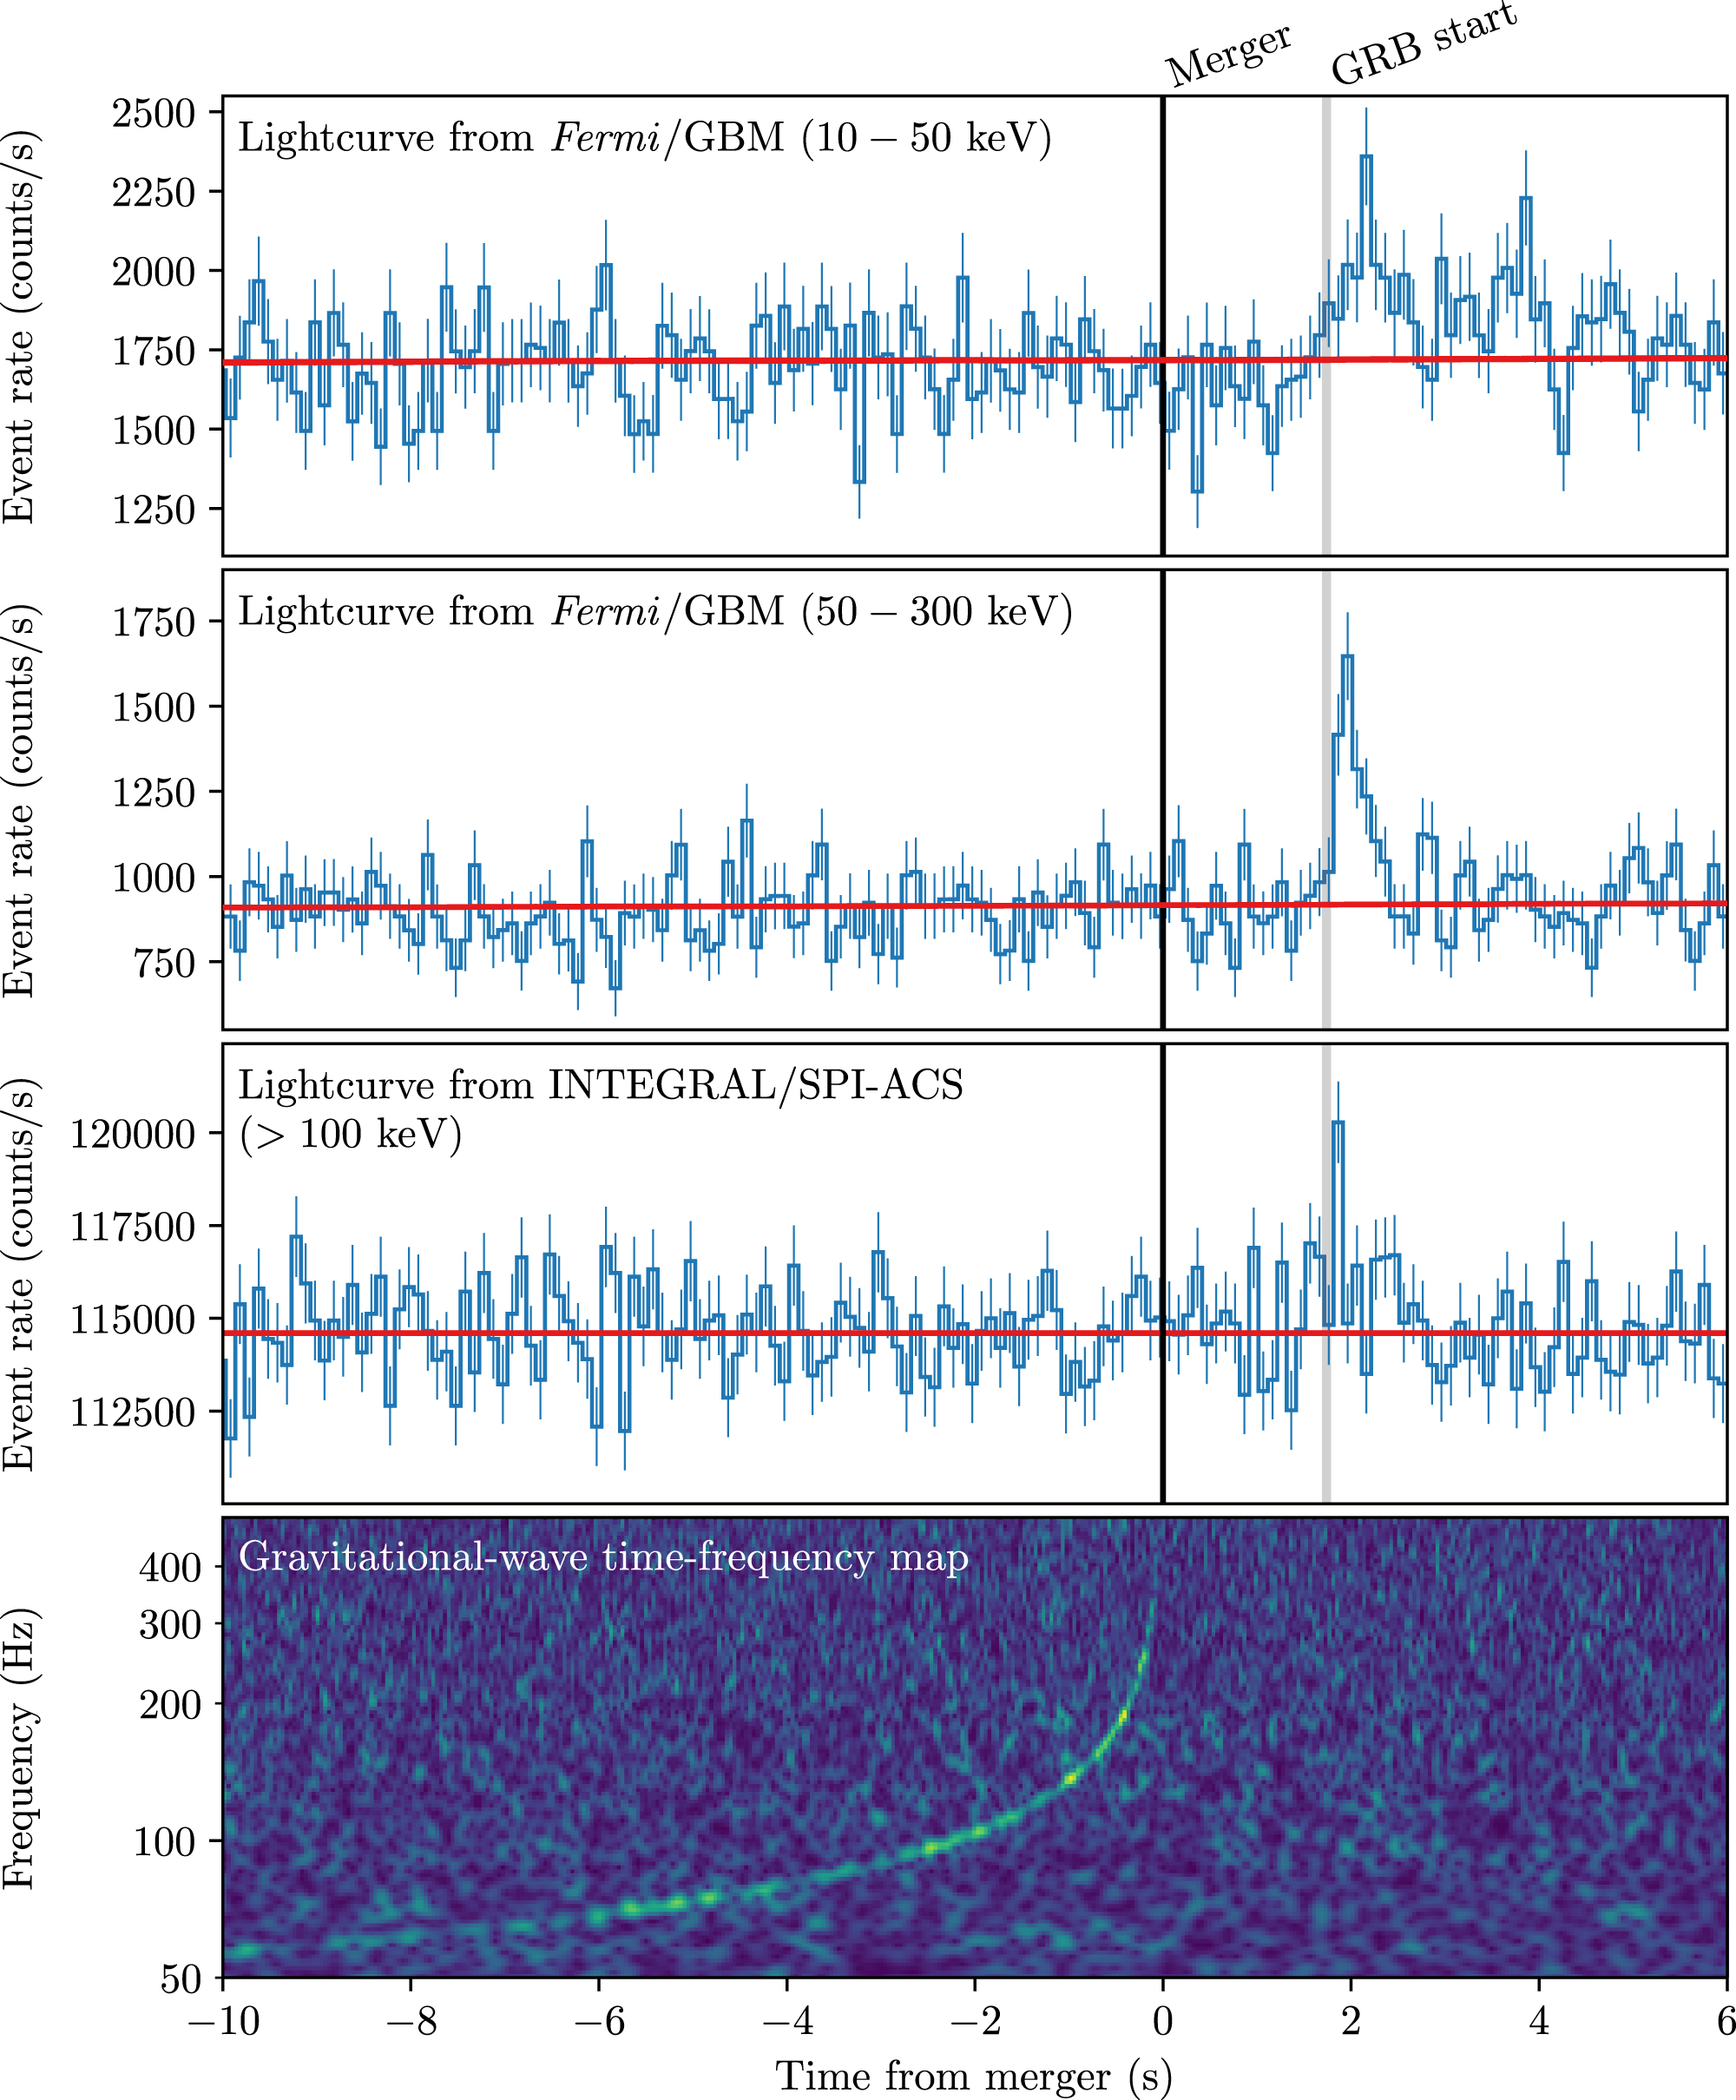
\includegraphics[width=0.8\linewidth]{grb-gw-170817.jpg}
\end{center}
\caption{\textbf{GRB170817A and GW170817.} Here we see that the a coherent conbination of the Hanford and Livingston strain data from GW170817 in the bottom panel. The top two panels shows the Fermi GRM curve in the 10-50keV and the 50-300keV range respectively. The INTEGRAL/SPI-ACS data is shown in the third plot. The background estimate for each detector is indicated by the red line. Note that the GRB was detected 1.7 seconds after the GW signal was detected. We can also see that Fermi detected a longer, softer signal in the 10-50 keV range, that lasted for a few seconds after the triggering pulse. \textbf{cite Gravitational Waves and Gamma-Rays from a Binary Neutron Star Merger: GW170817 and GRB 170817A} }
\label{fig:grb gw 170817}
\end{figure}

\subsection{Initial Observation and Followup}
The initial detection of GW 170817 was made only by the LIGO Hanford observatory, despite the fact that both LIGO detectors and the Virgo detector were in observing mode. A quick investigation found that the Livingston detector data had not been included by the low-latency search due to a glitch approximately 1.5 seconds before the coalescence phase of the signal. Glitches such as this happen at a rate of once every few hours in the LIGO detectors. These glitches are not temporally correlated between the two LIGO detectors and their source is unknown. Despite the glitch, the GW signal is clearly visible in the data (see the top panel of figure \ref{fig:l1 gltich}). 

\begin{figure} % Example of including images
\begin{center}
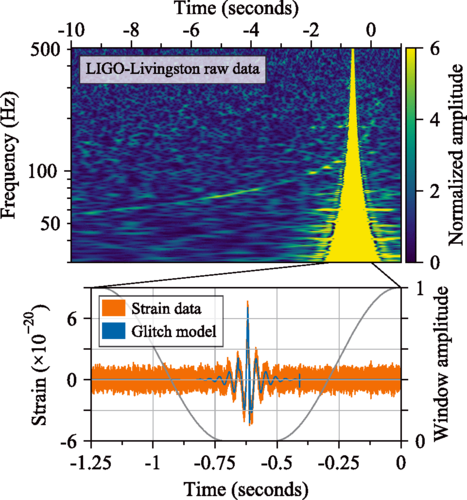
\includegraphics[width=0.8\linewidth]{l1_glitch.png}
\end{center}
\caption{\textbf{Glitch in the LIGO Livingston Observatory.} The top panel shows a time frequency map for the Livingston observatory data at the detection time of GW 170817. A glitch is clearly visible approximately 1.5 seconds before the end of the signal. Despite this the signal is still clearly visible. The bottom plot shows the raw strain data from the Livingston observatory. This data is bandpassed between 30 Hz and 2 kHz to emphasise the sensitive range of the detector. The grey curve (and right axis) shows the inverse Tukey window used to smoothly zero out the data around the glitch before the rapid reanalysis of the data. The blue curve shows the waveform model used to subtract the glitch from the data before measurements of the source's properties were made. \textbf{cite GW170817 observation from BNS} }
\label{fig:l1 gltich}
\end{figure}

Due to the coincidence with GRB 170817A, a rapid reanalysis of the data was performed, with the glitch removed from the data using an inverse Tukey window (see the bottom panel of figure \ref{fig:l1 gltich}). Removing a glitch like this lowers the reported SNR of a matched filter search compared to if there was no glitch, but allows the trigger to pass signal consistency tests\footnote{In fact, some offline analyses automatically gate out glitches, see section \ref{sec:pygrb improvements} and [\textbf{cite someone}]}. The data from the LIGO and Virgo detectors, with the Livingston glitch and some other noise removed, is shown in figure \ref{fig:170817 ifo strain}. The GW signal, clearly visible in the LIGO detectors, had an SNR of 18.8 in Hanford and 26.4 in Livingston, but an SNR of just 2.0 in Virgo.

\begin{figure} % Example of including images
\begin{center}
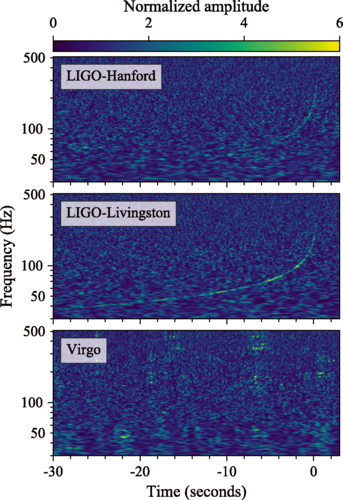
\includegraphics[width=0.8\linewidth]{gw170817_ifo_strain.png}
\end{center}
\caption{\textbf{GW 170817 Detection.} Here we see time frequency maps of the LIGO Hanford and Livingston observatories, and the Virgo observatory at the detection time of GW 170817. This data has been whitened and independently observable noise sources have been subtracted, including a glitch in the Livingston data. The non-detection by Virgo significantly reduced the amount of the sky that the signal could have originated from. \textbf{cite GW170817 observation from BNS} }
\label{fig:170817 ifo strain}
\end{figure}

The high SNR in the LIGO detectors compared to Virgo suggested that the GW originated from a part of the sky that Virgo was not sensitive to at the time of the trigger (see section \ref{sec:gw detectors}). The source of the GW was localised to within 31 deg$^2$ using the time delay between the LIGO detectors and the fact that the source originated from a null of the Virgo detector\footnote{For parameter estimation analysis of the signal, the glitch was modelled and subtracted from the data (see the bottom panel of figure \ref{fig:l1 gltich}), which reduced the sky patch to an area of 28 deg$^2$.} [\textbf{cite BNS detection paper}] and the sky localisation determined using GW data was consistent with the data determined by GRB detectors (see figure \ref{fig:170817 skymap}). GW data also determined the distance to the source was approximately 40 Mpc, close enough that relatively complete galaxy catalogues exist. Using this information, ground based observatories began scanning the sky patch for an afterglow. Less than 11 hours after the initial trigger, the Swope telescope in Chile, followed by five other observatories  [\textbf{cite kilonova paper?}], found a new object on the edge of galaxy NGC 4993 (see figure \ref{fig:NGC4993}). 


\begin{figure} % Example of including images
\begin{center}
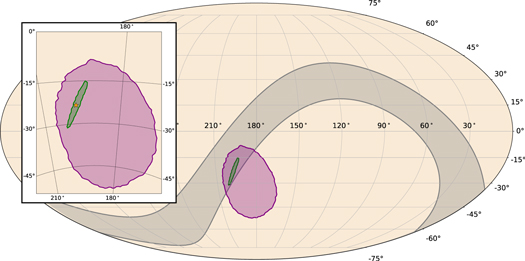
\includegraphics[width=0.8\linewidth]{gw-grb-170817-sky-map.jpg}
\end{center}
\caption{\textbf{Sky map for GW170817/GRB170817A.} Here we see the 90\% confidence sky localisation for the LIGO and Virgo collaborations in green, the GBM 90\% localisation in purple, and the annulus formed by Fermi and INTEGRAL timing information in grey.  \textbf{cite Gravitational Waves and Gamma-Rays from a Binary Neutron Star Merger: GW170817 and GRB 170817A} }
\label{fig:170817 skymap}
\end{figure}

\begin{figure} % Example of including images
\begin{center}
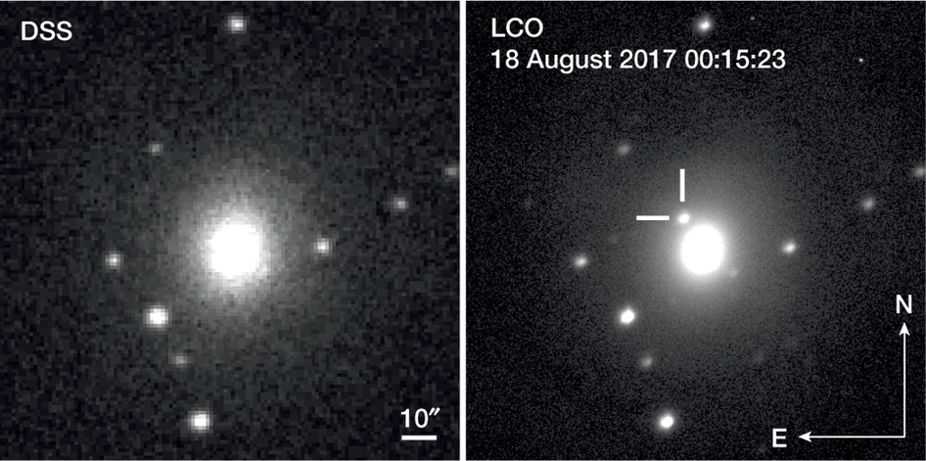
\includegraphics[width=0.8\linewidth]{NGC4993.jpg}
\end{center}
\caption{\textbf{NGC 4993.} Image of NGC 4993 taken in 1992 by the Anglo-Australian Observatory (left) and August 18th 2017 by the Las Cumbres Observatory (right). \textbf{cite https://www.nature.com/articles/nature24291/figures/2} }
\label{fig:NGC4993}
\end{figure}

\subsection{Kilonova Observation}
This new object was studied intensely over the following days. The transient was initially observed to be a rapidly fading blue transient, which had faded completely within 48 hours. The spectrum showed no supernova-like absorption lines, ruling out the possibility that this transient was caused by a supernova. Over the next $\sim$10 days the spectrum grew redder, and observations by ESO-VLT/X-shooter showed evidence of the decay of r-process elements. This all strongly indicates that the transient was a kilonova. X-ray emission was detected 9 days after the merger, and radio emission after 16 days. This delayed radio emission was predicted from neutron star merger models as the ejecta interacts with the interstellar medium.

\subsection{Structured Jets} \label{sec:structured jets}
GRB 170817A was significantly fainter than any other detected GRB (see figure \ref{fig:brightness_z}). In fact, the GRB showed no evidence for photons with energy $>511$ keV, i.e. above the pair production threshold, meaning that the matter ejected from this GRB need not have been traveling at relativistic velocities\footnote{Recall from section \ref{sec: fireball} that GRBs were assumed to accelerate matter to relativistic velocities as this would explain how GRBs could emit photons above the pair production threshold. The fact these high energy photons were not detected means that material ejected from this GRB need not travel at relativistic velocity}. There are several factors that affect GRB brightness, such as the angle the GRB is observed at and the intrinsic properties of the jet. The simplest model of the jet is the \textit{top-hat jet}, which has a uniform core that terminates sharply at some angle from the GRB axis. It is possible that GRB 170817A was a top-hat jet viewed off-axis, making it appear dimmer. Another possibility is that the GRB had a \textit{structured jet}, meaning that it gradually becomes less energetic as the angle from the axis increases. It is also possible that the GRB jet had a \textit{cocoon} created by the relativistic jet shocking the non-relativistic matter surrounding the jet. These three possibilities are shown in figure \ref{fig:jet}. It could also be that GRB 170817A was produced by a new mechanism that is not observable at greater distances as it is intrinsically dim. It could also be that GRB 170817A is part of a population of subluminous GRBs that can only be detected if they occur unusually close or that the GRB was not jetted at all, and is a mildly relativistic, isotropic fireball. In this section we will consider each of these possibilities and compare each model to the observed spectral evolution of GRB 170817A, from the prompt emission to the late afterglow observations. We will see that the best explanation for the faint prompt emission of GRB 170817A is that it had a structured jet seen at a relatively large viewing angle. 

\begin{figure} % Example of including images
\begin{center}
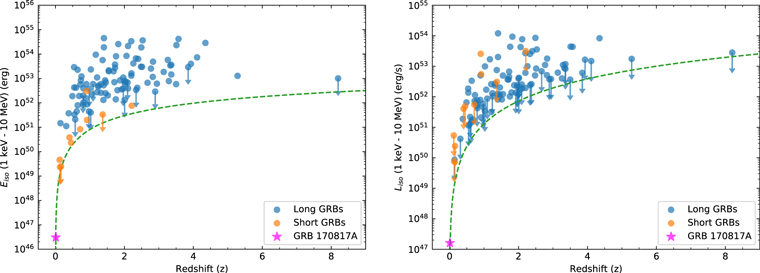
\includegraphics[width=1.0\linewidth]{grb_z_brightness.jpg}
\end{center}
\caption{\textbf{Brightness/Luminosity against redshift.} Here we see the distribution of $E_\text{iso}$ and $L_\text{iso}$ against redshift for every GBM-detected GRB with a measured refshift. For GRBs with power law spectra, marked with a downward pointing arrow, this is taken to be an upper limit. This is because the spectra must have curvature, and so extrapolating a power law leads to an overestimation. The green dashed line shows the approximate detection threshold for the GBM. These plots show that GRB 170817A was much dimmer than any other detected GRB. [\textbf{cite GRB BNS paper}] }
\label{fig:brightness_z}
\end{figure}

\begin{figure} % Example of including images
\begin{center}
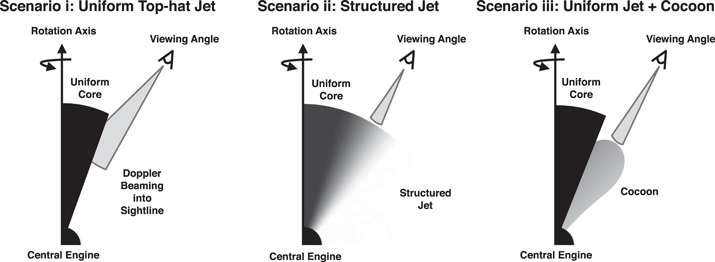
\includegraphics[width=1.0\linewidth]{jet_structure.jpg}
\end{center}
\caption{\textbf{Jet Structure Scenarios.} Three different scenarios that could explain the low luminosity of GRB 170817A. The first scenario is that a Top-hat jet was viewed off-axis. The second is that the jet is structured, with photons emitted further from the axis being lower energy and fewer in number, and viewed relatively far from the axis. The third scenario is that a uniform jet has a surrounding cocoon that emits lower energy photons, and it was these lower energy photons that were detected. \textbf{cite GRB BNS paper} }
\label{fig:jet}
\end{figure}

We begin by using some simple arguments to show some of these models are unlikely. The observed gamma-ray properties of GRB 170817A are similar to other short GRBs, making it unlikely that the prompt emission was caused by a different mechanism to other short GRBs. It is also unlikely that GRB 170817A represents the first detected member of a subluminous population as this would mean short GRB luminosities covers six orders of magnitude, which is difficult to conceive given the small range of physically possible neutron star masses. Though it should be noted that a wider range of intrinsic luminosities is possible if we assume that some short GRBs are produced by NS-BH mergers, or that the magnetic field strength of GRB progenitors is highly variable and significantly affects the intrinsic luminosity [\textbf{cite BNS GRB paper}].

This leaves only those models that focus on the jet structure and viewing angle of the prompt emission. In [\textbf{cite afterglow paper}] they compare the late time afterglow observations of GRB 170817A to the predictions made assuming three different jet models: A top-hat jet seen off-axis, a structured jet with a cocoon, and a mildly relativistic, isotropic fireball. The expected afterglow for a structured jet GRB is very different to the off-axis top-hat and the isotropic fireball. For a structured jet, the initial afterglow emission will be due material traveling down the line of sight. After a few days, this material will interact with the interstellar medium, causing it to decelerate and emit light. Over the next months, material ejected at an increasing large angle from the line of sight will become observable due to interactions with the interstellar medium, causing the afterglow to appear brighter. Eventually, on a timescale of months or years, the jet will become observable. At this point the afterglow will have reached peak luminosity and will start to fade. This is qualitatively different to the top-hat and isotropic fireball case, in which all ejected material has approximately the same energy and so the afterglow rises more rapidly and fades more slowly, unlike the afterglow of a structured jet GRB which will rise slowly (see top right panel of figure \ref{fig:structured jet}). Note that if the jet is observed on axis, then the afterglow of a structured jet would be indistinguishable from a top-hat jet as the afterglow would peak quickly and then fade in both cases. In [\textbf{cite afterglow paper}] the authors use Markov Chain Monte Carlo to fit the structured jet, top-hat, and isotropic fireball model to the spectra of GRB 170817A. The 3 GHz light curve for the best fit of each model is plotted in figure \ref{fig:model comparison}. We can see that the structured jet model fits the data much better than either the top-hat or isotropic fireball model. The best fit model viewing angle is $\theta = 33^{+4}_{-2.5}$, which is comparable to the LIGO measurement of $\leq 28^\circ$. If this model of the structured jet is correct,\footnote{The best fit structured jet model has a $\chi^2$ of 69 for 56 degrees of freedom and a probability of p=$11\%$.} then approximately one in every 20 BNS systems detected with GWs should have a GRB counterpart [\textbf{cite afterglow paper}]. 

The structured jet model also has the advantage of being a natural consequence of binary neutron star mergers. As the jet shocks the slow moving material in the surrounding area, a cocoon of high pressure, subrelativistic matter will form. This cocoon creates a sheering force on the jet which creates a jet with a highly relativistic core, surrounded by lighter and slower moving material, with mildly relativistic wings at larger angles (see left panel of figure \ref{fig:structured jet}). 

\begin{figure} % Example of including images
\begin{center}
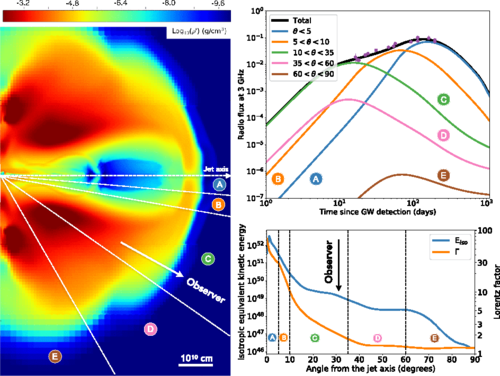
\includegraphics[width=1.0\linewidth]{structured_jet.png}
\end{center}
\caption{\textbf{Structured Jet.} Left panel: A pseudocolour density image of the simulation used to compute the afterglow curves [\textbf{citation in afterglow paper}]. The low density core of the jet is the blue region near the middle. The orange and green region around the core is the slow moving wings.  Top right panel: Here we see the 3 GHz flux detected from different parts of the structured jet as time progresses. The angle is relative jet axis, so the blue curve is the core of the jet, the orange curve is the fast wings of the jet, the orange curve is the material moving along the line of sight (an angle of about $33^\circ$ in this case), and the pink and brown curves correspond to large angles, that do not contribute much to eh observed flux. Bottom right panel: The distribution of energy as a function of angular separation from the jet. \textbf{cite GRB afterglow paper paper} }
\label{fig:structured jet}
\end{figure}

\begin{figure} % Example of including images
\begin{center}
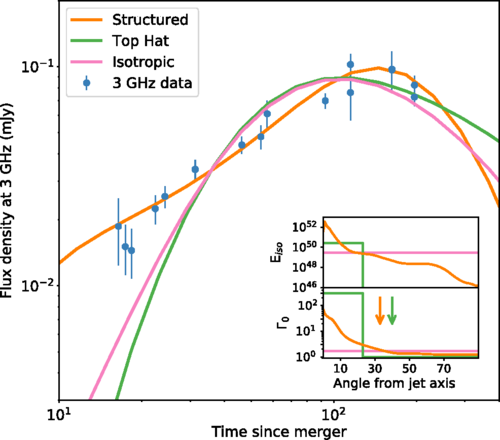
\includegraphics[width=1.0\linewidth]{grb_model_comparison.png}
\end{center}
\caption{\textbf{Jet Model Comparison.} Here we see a comparison of the best fit for the structured jet, Top-hat jet seen off-axis, and isotropic models. The afterglow's measured flux density at 3 GHz is shown by the blue symbols (though the fits were performed with multiwavelength data). The inset shows the best fit isotropic energy and Lorentz factor for each model as a function of viewing angle. The arrows show the position of the observer for the structured and Top-hat jet models. \textbf{cite GRB afterglow paper paper} }
\label{fig:model comparison}
\end{figure}

\subsection{Other Scientific Results}
We have so far focused on the physics of the jet and the progenitor of the GRB as these both effect our interpretation of the coincident GRB/GW signal. Now that we are confident that GRB 170817A resulted from a binary neutron star merger, we can use it as a probe for other physics. 

\subsubsection{Speed of Gravity}
One result that can be derived immediately from the coincident detection is the speed of gravity $\nu_\text{GW}$. General relativity predicts that GWs will travel at the speed of light $\nu_\text{EM}$. We can now test this prediction by using the measured time delay between GW and GRB detection and different assumptions of time delay between the merger and GRB emission. The greater the distance to the GRB, the less the uncertainty in time delay. For this reason we will assume the GRB happened at a distance $D = 26$ Mpc, the lower bound of the $90\%$ credible distance determined from the GW signal.  The delay between the peak of the GW signal and the start of the start of the GRB signal is $1.74 \pm 0.05$ seconds. We can find an upper limit on the speed of gravity by assuming that the first photons were emitted at merger time. This means the entire time delay is due to GWs traveling faster than light. Using the upper limit for the time delay, this gives us $\delta t = 1.74 + 0.05$. For a lower limit we can assume a significant delay between the merger and the first photons being emitted. It can be shown that the duration of a GRB is approximately the time delay between the merger and the GRB emission [\textbf{cite GRB BNS paper}]. It is therefore expected that the time delay between merger and emission is also $\sim2$ seconds. For a lower bound, we conservatively assume a time delay of $\Delta t = 10 - 1.74 + 0.05= 8.31$ seconds. As $\Delta \nu /\nu_\text{GW} = -\nu_\text{EM}\Delta t/D$, where $\Delta \nu = \nu_\text{GW} - \nu_\text{EM}$, we find
\begin{equation}
-3 \times 10^{-15} \leq \frac{\Delta \nu}{\nu_\text{GW}} \leq +7\times 10^{-16} \fs
\end{equation}
As this range includes zero, it is in agreement with general relativity. The largest source of uncertainty in this calculation is the time delay between GW and EM emission. As this does not depend on the distance to the source, more joint detections will allow this value to be constrained. This will allow for more accurate measurements of the speed of gravity and rule out more exotic EM emissions mechanisms, some of which predict time delays much greater than the 10 second bound we used in the above calculation.
\begin{itemize}
\item Speed of GW inequality is different to the GRB paper, but I don't really understand the approximation used there \textbf{ASK PATRICK}
\end{itemize}

\subsubsection{Hubble Constant}
Another scientific result to come from GW 170817 is a new measurement of the Hubble constant. Using the distance inferred from GW data, and the redshift measurement of the associated galaxy NGC 4993, it is possible to calculate the Hubble constant directly, instead of using a cosmic distance ladder.\footnote{The cosmic distance ladder describes the fact that various different techniques are used to measure distances depending on the distance scale being measured. Each technique is useful for a certain range of distances, and the different techniques overlap in some distance range, allowing them to be calibrated to one another.} Using this method, the Hubble constant was measured to be $H_0 = 70^{+12}_{-8} \text{ km s}^{-1} \text{Mpc}^{-1}$. This is consistent with measurements made using both Planck data and standard candles. 

\subsubsection{Rates}
This detection can also be used to predict rates of BNS mergers and joint GW/GRB mergers. We will cover this in more detail in section \ref{sec:pygrb o2 results}, where we consider not only the detection of GRB 170817A and GW 170817, but also the 41 non-detections for other GRBs for which there was GW data available. There we will see that the expected rate of BNS mergers is 1-30 per year, with about 0.07-1.80 joint GRB-GW detections per year for the 2019-20 observing run.


\section{GRB Progenitors} \label{sec: grb prog}
In section \ref{sec:GRB history} we discussed the evidence for short GRBs being produced by neutron star mergers and long GRBs being produced by core collapse supernova. In both of these cases, a large amount of energy is displaced rapidly from a small region. In section \ref{sec: fireball} we discussed  the fireball model, which shows that these circumstances cause shocks and relativistic beaming which explain the high energy and variability of GRBs. But the fireball model only assumes that the \textit{central engine}, the source of energy for the GRB, is small and highly energetic. There are many phenomena that satisfy this criteria. In this section we discuss some of these possibilities. We will see under which circumstances neutron star mergers and core collapse supernovae can power short and long GRBs respectively.

\subsection{Compact Binary Coalescence}
As mentioned previously, short-hard GRBs are thought to be powered by the CBC involving at least one neutron star, with a neutron star or black hole as the other component of the binary. With the detection of GW170817 in conjunction with GRB170817A, we now know this is the case for at least some short-hard GRBs. In this section we will discuss the immediate aftermath of a NS merger and the different GRB and GW signals that each could be produced.

\paragraph{NSBH Mergers} The simplest case is that of an NSBH merger where the BH mass is significantly greater than that of the NS. If the BH to NS mass ratio is greater than 5:1 then the innermost stable circular orbit (ISCO)\footnote{The ISCO is the smallest stable circular orbit for a test particle around a BH.} is greater than the tidal disruption radius\footnote{The radius around a BH where the BH's tidal forces pull apart an in-falling star.}. This results in the NS being swallowed whole by the BH and leaving no accretion disk. The accretion disk is believed to be essential in powering a GRB after a NS merger, and so this case is not expected to produce a GRB. If the NSBH has a relatively low mass ratio, then the neutron star will be tidally disrupted before merging with the black hole. This will create a massive accretion disk and is expected to produce a GRB. 

\paragraph{BNS Mergers} For BNS mergers we must consider both the mass ratio and the total mass of the system. This is because it is possible for the merging neutron stars to either form a black hole or a \textit{hypermassive neutron star} depending on the total mass of the binary system. The simplest of these is for a system with approximately equal mass ratio and a high total mass, such that a black hole can be produced immediately after merger. This requires the total mass to be above about 2.9$M_\odot$ [\textbf{cite}], but the exact value depends on the EOS of neutron stars. In this case, no accretion disk will be produced and so no GRB is expected. 

For an unequal mass ratio, the lighter neutron star is tidally disrupted by the larger neutron star. Matter from the lighter neutron star then accretes onto the more massive star, causing the more massive star to collapse into a black hole. This can potentially leave a massive accretion disk which could power a GRB.  

If the total mass is less than about 3$M_\odot$ [\textbf{cite}] then the merger is not expected to immediately form a black hole but to instead form a hypermassive neutron star. This is a neutron star that is supported by differential rotation and thermal pressure. The merger will produce an accretion disk which could power a GRB. It is also possible that the rapidly rotating hypermassive neutron star will be ellipsoidal in shape, making a powerful emitter of GWs. These GWs would be detectable with aLIGO up to about 20Mpc [\textbf{cite}]. Over time, the hypermassive neutron star will lose angular momentum due to GW emission and magnetic force, its rotation will become more uniform due to magnetic forces and viscosity, and it will radiate away it's heat. These factors cause the hypermassive neutron star to eventually collapse to a black hole. This can happen on a timescale as short as milliseconds [\textbf{cite someone}] up to seconds or minutes[\textbf{citation in BNS GRB paper}]. 

\subsection{Core Collapse}
Long GRBs are known to be caused by core collapse supernova. In this section we will discuss some of the possible central engines for long GRBs, focusing on those that could produce a GW signal strong enough to be detected with aLIGO. 

\paragraph{Rotational Instabilities of Proto-Neutron Stars} 
The cores of stars with initial masses in the range $10M_\odot \lesssim M \lesssim 25M_\odot$ are expected to collapse to rapidly rotating \textit{protoneutron stars}; stars which are cooling and contracting to form a neutron star. These protoneutron stars could exhibit non-axisymmetric deformations due to, for example, their rapid rotation driving hydrodynamic instabilities.  The rapid rotation of the star could then drive significant GW emission, potentially detectable to 10 Mpc with current detectors and even further if the protoneutron star accretes supernova material. 

\paragraph{Non-axisymmetric Instabilities of Accretion Disks}
For stars with initial mass greater than $\sim 30M_\odot$, the core collapse of the star will form a central black hole surrounded by an accretion disk. If the accretion disk has sufficiently high angular momentum and non-axisymmetric instabilities, then it can produce detectable GWs with a waveform similar to that of a low mass binary merger. For a stellar mass black hole with a clump of matter in its accretion disk of approximately $0.1M_\odot$, an accretion disk instability can potentially be detected out to 100Mpc with aLIGO [\textbf{cite something}]. An accretion disk instability can be caused by, for example, a high angular momentum such that the accretion disk is not gravitationally stable. 

\section{GRB Detectors} \label{sec:grb detectors}
Most GRB detections have been come from the Swift and Fermi space telescopes, or a network of satellites called the Interplanetary Network. In this chapter we discuss the characteristics of these three missions, focusing on the aspects that affect a followup search for gravitational waves: sky coverage, source localisation, and sensitive energy range. 

\subsection{Swift}
The Swift satellite is named for its ability to autonomously repoint itself towards a GRB within 90 seconds. It has three instruments: The first is the \textit{Burst Alert Telescope} (BAT), the primary tool for GRB detection. It has a large field of view of approximately 2 steradians, and is highly sensitive in the 15-150 keV energy range. The BAT can localise GRBs to within 1-4 arcminutes. The other two instruments are the \textit{X-ray Telescope} (XRT) and the \textit{UV/Optical telescope} (UVOT). These are used for followup observations of the GRB afterglow. They can also reduce the sky-error; XRT can localise to 3-5 arcseconds and UVOT to 0.5 arcseconds \textbf{cite \url{https://swift.gsfc.nasa.gov/about_swift/}}. The UVOT is also used to determine the redshift of the host galaxy from which the GRB originated. To date, Swift has detected over 1000 GRBs, with approximately $10\%$ of these having $T_{90}<2s$ \textbf{cite \url{https://swift.gsfc.nasa.gov/archive/grb_table/stats/}}

\subsection{Fermi}
The Fermi Satellite [\textbf{cite \url{https://www.nasa.gov/content/fermi/overview}}] has two instruments: The first is the \textit{Large Area Telescope} (LAT), and the second is the \textit{Gamma-ray Burst Monitor} (GBM). The LAT is sensitive to higher energy photons (in the range 30 MeV-300 GeV), has sky coverage of  2 steradians, and can localise to within 1 arcminute of accuracy. The GBM is sensitive to lower energy photons (in the range 8keV-30MeV), is sensitive to a greater sky area that LAT (9.5 steradians), but cannot localise as well LAT (typically 10s or 100s of square degrees). 

\subsection{The InterPlanetary Network}
The interplanetary network (IPN) [\textbf{cite something}] is a network of GRB detectors on spacecraft that are in low Earth orbit, eccentric Earth orbit, traveling to other planets, or orbiting other planets already. None of the spacecraft in the IPN are dedicated GRB detectors; they are individually unable to determine the sky position of a GRB and are not as sensitive as dedicated GRB detectors. But the network as a whole acts as an all-time all-sky GRB monitor. And as the spacecraft are great distances apart, the network can triangulate sky position to within several arcminutes. The accuracy is greatly dependent on the number and position of the satellites that detect the GRB, with satellites at greater distances significantly improving the sky location error. A list of past and current IPN satellites can be found here [\textbf{cite \url{https://heasarc.gsfc.nasa.gov/W3Browse/all/ipngrb.html}]}.

\section{GRB Gravitational Wave Search Strategies}
In chapters \ref{chap: CBC} and \ref{chap: mva}, we discuss in detail two search pipelines for the CBC and burst search respectively. It is useful before discussing these searches to give an overview of the general strategy when searching for GWs associated with GRBs. This will give context to later discussions on the details of the searches, and also to the following section on the astrophysics that can be learned from detections of GWs from GRBs. 

\subsection{Triggered and Untriggered Searches}
We can classify GW searches as being either \textit{triggered} or \textit{untriggered}. Untriggered searches will search all of the sky for all of the time when there is detector data. These all-sky all-time searches can be further divided into groups depending on the amount of time they take to run. Some searches, for example [\textbf{cite PyCBC live, gstlal, CWB papers}], are untriggered and low latency. They aim to find GW triggers and their sky position within minutes, allowing astronomers to followup the trigger. This is what happened for GW 170817, which was detected in low latency, in coincidence with a Fermi GRB, and followed up by ground and space based observatories. High latency untriggered  searches, such as [\textbf{cite pycbc, gstlal papers}], work on much longer timescales, as long as months, but aim to achieve very high sensitivity with very low false alarm rates. These pipelines are more sensitive and have lower false alarm rates than the low latency searches. 

Triggered searches use sky location and time information from other messengers, such as GRBs. These searches have the advantage of only needing to analyse a limited amount of data (as the trigger time is known) and being able to use information gleaned from the other messengers to restrict the search. For example, both long and short GRBs are suspected to emit their jets along the axis of angular momentum, which can be used to infer than the GRB is circularly polarised (see section \ref{sec:circ pol}). 

Results from both triggered and untriggered searches can be used in \textit{Multimessenger} searches [\textbf{cite subthreshold paper}]. These searches attempt to combine subthreshold triggers from multiple different messengers to make a confident detection. For example, a core collapse supernova could produce a long GRB, a GW signal, and neutrinos, but be too distant for any search using just one of these messengers to make a confident detection. 

\subsection{Modeled and Burst Searches}
Searches for GWs can also be classified as either \textit{modeled} or \textit{burst}. Modeled searches have theoretical models of the waveforms they are searching for. For example, CBC signals can be modeled by numerical relativity and analytic methods [\textbf{cite something}]. These waveforms can then be used to build a more sensitive search, such as a matched filter search (see sections \textbf{list matched filter sections}). In chapter \ref{chap: CBC} we will look at PyGRB, a targeted, modeled search for GWs associated with GRBs. 

Burst searches use minimal assumptions about waveform morphology, instead relying on measures of coherence between detector data streams. This is in general less sensitive than if a waveform was known and a matched filter search could be carried out, but there are no such waveform models for supernovas/long GRBs. In chapter \ref{chap: mva} we will discuss a burst search called Xpipeline. 

\section{GRB Astrophysics with Gravitational Waves}
We have discussed what GRBs are, what causes GRBs, and seen that they are good emitters of GWs. We end this chapter with a discussion of how GW astronomy will add to our understanding of GRBs. 

\paragraph{Short GRB Progenitors}
With the coincident detection of GRB 170817A and GW 170817, it is now known that at least some short GRBs are produced by neutron star mergers. As more detections are made it will become easier to determine whether this is the only source of short GRBs or if other mechanisms exist. Also, by comparing the electromagnetic counterpart to the knowledge gleaned from the GW signal about the binary, such as whether the system is an NSBH or a BNS, we can learn more about the central engine of the GRB. 

\paragraph{Long GRB Progenitors}
There is a lot of evidence that at least some long GRBs are powered by core collapse supernova. If this is the case, then it should be possible to detect GWs in coincidence with a nearby long GRB. The GW signal would provide clues as to the evolution of the core collapse. If there is no GW detection, then it is possible to constrain the dynamics of the core collapse. Supernovae searches performed by LIGO at the moment only analyse supernovae that occur at a distance of less than 20 Mpc, and have so far seen no GW signal. This null result has been used to rule out some of the more extreme GW emission models for supernovae. [\textbf{cite O2 supernova paper}]

\paragraph{Populations}
There are many unknowns about the populations of short GRBs and compact binary systems. As a network of GW detectors is essentially sensitive to the whole sky, it will be possible to better understand the population of compact binary systems within the well defined horizon of the detectors network. As GW signals also allow the direct inference of distance, it will even be possible to understand how the population of binary systems changes with distance up to the horizon of the detector network.\footnote{Due to the limited horizon of aLIGO and the low rate of neutron star mergers, this will have to wait for third generation GW detectors.} With the detection of GW 170817, the local BNS merger rate is measured to be $1210^{+3230}_{-1040}$ [\textbf{cite catalog paper}]. This would correspond to a joint GRB/GW detection rate of between 0.07 and 1.80 events per year for the 2019/20 LIGO/Virgo observing run [\textbf{cite O2 GRB paper}]. 

\paragraph{GRB Distance and Luminosity}
For CBC GW signals where the inclination is approximately known, such as those associated with short GRBs, the distance to the source can be determined directly from the GW signal and without using a cosmological distance ladder. This allows independent verification of distances, as was done with GRB 170817A and GW 170817. Once the distance is known, the luminosity of the GRB can reconstructed. This can also be used to as an alternative measure of Hubble's constant, again, as was done for GW 170817 [\textbf{cite paper}]. 

\paragraph{Jet Structure}
By comparing the rate of joint GW/GRB detections of BNS and NSBH mergers to the number detected through GWs alone, it will be possible to determine the opening angle of short GRBs. For the structured jet discussed in section \ref{sec:gw170817}, it is estimated that one in twenty BNS GW detections will have a GRB counterpart [\textbf{cite afterglow paper}]. For strong GW signals, it will also be possible to measure the polarisation of the GW. If the GW is face on, then it will be circularly polarised, but if it is edge on then it will be elliptically polarised. By measuring the polarisation of a large number of short GRBs and studying their prompt emission, it will be possible to fully describe the angular structure of short GRB jets. 

\paragraph{Neutron Star Equation of State}
The equation of state (EoS) of matter at neutron star densities is poorly constrained. There are many ways that studying the GW signal of neutron star binaries can be used to determine the EoS. For example, a GW signal for a system with a neutron star of mass $\sim 2M_\odot$ suggests a stiff EoS as a soft EoS could not support such a massive star. Another way of constraining the EoS of neutron stars is to look at the orbital frequency of a neutron star binary when tidal disruption occurs, as this depends on the radius of the neutron star. Using this radius with the mass of the neutron star (as determined by the inspiral waveform), we can determine the density of the neutron star. Tidal deformation can also affect the inspiral part of the waveform [\textbf{cite same paper as bartos paper}]. It has been shown [\textbf{cite Read et al}] that the advanced LIGO detectors can determine the radius of a neutron star to within $\sim 1$km for a source at 100 Mpc. It has also been theorised that the core of neutron stars may be made of strange quark matter. If this is true, then it will have a significantly different GW signal for both CBC systems [\textbf{cite same paper as bartos paper}] and neutron star instabilities after a core collapse supernova. Thus, GW astronomy can determine if neutron stars contain quark matter cores. 


\chapter{A Targeted Search for Gravitational Waves associated with Short GRBs} \label{chap: CBC}
\section{Introduction}\label{CBCintro}
Compact binary coalescence (CBC) events are strong emitters of gravitational waves (GWs), and many searches exist to search for signals from these systems [\textbf{cite pycbc gstlal and any others}]. These searches take theoretical waveforms [\textbf{cite someone}] and matched filter them against the strain data from GW detectors (\textbf{ref matched filter section}). It is known that the progenitor of at least some short GRBs are compact binaries, either binary neutron star (BNS) or low mass ratio neutron star - black hole (NSBH) systems. While the search pipelines mentioned above can detect the signals associated with short GRBs, they do not use any of the EM information that GRB detectors collect as they search for binary black hole (BBH) systems as well as neutron star mergers. By combining the EM information from GRB detectors with the strain data from GW detectors, we can make a more sensitive search specifically designed to look for CBC signals associated with short GRBs. This is what PyGRB was developed to do.

There are several ways EM information can improve a GW search. The first is that the time and sky position of the short GRB are known from GRB detectors. This not only means that the analysis can run on less data but this information can also be used to make a more powerful detection statistic, which we will see in section \ref{sec:coh snr}. We can also assume that the binary system that produced the GRB was face on, as GRBs are emitted perpendicular to the orbital plane. We will see in section \ref{sec:circ pol} that this can also be used to improve the detection statistic.  

In this chapter we describe PyGRB [\textbf{cite all the papers}], a targeted matched filter search for short GRBs. PyGRB is integrated into the PyCBC data analysis software [\textbf{cite pycbc technical paper}], which is primarily an all-time, all-sky, matched filter search for CBC signals. We will begin with an overview of the PyCBC pipeline, as this is the foundation that PyGRB is built upon. In section \ref{sec:PyGRB} we discuss the theory behind the statistics used by PyGRB and show why it is more sensitive to GRB signals than the all-sky, all-time search. In section \ref{sec:pygrb workflow} we will see how this theory is applied to make a functioning search pipeline. We end this chapter with a discussion on the findings of PyGRB in the second advanced LIGO and advanced Virgo observing run.


\section{Coherent Matched Filtering} \label{sec:PyGRB}
In this section we will discuss the theory behind PyGRB; a targeted, matched filter search for GWs associated with short GRBs. The detection statistic of PyGRB is the \textit{coherent SNR}, which uses the sky position and time of the GRB, as well as the antenna response function and PSD of each detector in the network. Using these, it is possible to calculate the amount of signal power expected in each detector. For example, if a GRB was localised to a point in the sky directly above the most sensitive interferometer in the network, then this detector would be expected to have the highest SNR of all detectors in the network. If one of the other detectors in the network has a higher SNR, then it is less likely that this trigger is a true GW signal. Triggers with the expected ratio of signal power in each detector will have a higher coherent SNR than those that do not. 

This qualitative description of coherence is made rigorous in the following sections up to \ref{sec:coh snr}. In section \ref{sec:null snr} we discuss the \textit{null SNR}, another coherent statistic that measures the energy inconsistent with a GW. Short GRBs are expected to be emitted perpendicular to the orbital plane of the neutron star merger and with an opening angle of $30^\circ$ (see sections \ref{sec:jets} and \ref{sec:structured jets}). In section \ref{sec:circ pol} we will see how this information can be used to build an even more sensitive detection statistic. We then end this section by discussing how to reject non-Gaussianities in the data by using signal consistency checks.

\subsection{A Coherent Search for Coalescing Binary Systems}
\begin{itemize}
\item Show where the A's come from (don't know how to do this yet)
\end{itemize}

\subsection{Binary Coalescence Waveform} 
PyGRB searches for CBC signals with circular orbits and aligned spin components. These waveforms depend on 11 parameters: The two component masses $M_1$ and $M_2$, the component spins, the sky location $(\theta, \phi)$, the distance $D$, the coalescence time $t_0$, the orientation $\iota$, the polarisaton angle $\psi$, and the coalescence phase $\phi_0$. We can reduce to nine parameters if we assume the sky position is known. Of these, the distance, binary inclination, polarisation, and coalescence phase affect the phase and amplitude of the waveform and not the signal morphology. That is, the waveform can be written as
\begin{equation} \label{hp}
h_+(t) = \mathcal{A}^1 h_0(t) + \mathcal{A}^3 h_{\pi/2}(t)
\end{equation}
\begin{equation} \label{hx}
h_\times(t) = \mathcal{A}^2 h_0(t) + \mathcal{A}^4 h_{\pi/2}(t)
\end{equation}
where $h_0(t)$ and $h_{\pi/2}(t)$ describe the two phases of the waveform, are usually assumed to be orthogonal, and depend only on the component masses. The amplitudes $\mathcal{A}^i$ are given by 
\begin{equation} \label{A1}
\mathcal{A}^1 = \frac{D_0}{D} \left( \frac{(1+\cos^2 \iota)}{2} \cos 2\phi_0 \cos 2\psi -  \cos \iota \sin 2 \phi_0 \sin 2\psi \right)
\end{equation}
\begin{equation}
\mathcal{A}^2 = \frac{D_0}{D} \left( \frac{(1+\cos^2 \iota)}{2} \cos 2\phi_0 \sin 2\psi +  \cos \iota \sin 2 \phi_0 \cos 2\psi \right)
\end{equation}
\begin{equation}
\mathcal{A}^3 = -\frac{D_0}{D} \left( \frac{(1+\cos^2 \iota)}{2} \sin 2\phi_0 \cos 2\psi +  \cos \iota \cos 2 \phi_0 \sin 2\psi \right)
\end{equation}
\begin{equation} \label{A4}
\mathcal{A}^4 = \frac{D_0}{D} \left( -\frac{(1+\cos^2 \iota)}{2} \sin 2\phi_0 \sin 2\psi +  \cos \iota \cos 2 \phi_0 \cos 2\psi \right)
\end{equation}
where $D_0$ is used to scale the amplitude of the waveforms. For any $\mathcal{A}^\mu$ we can invert equations \ref{A1}-\ref{A4} to obtain the physical parameters up to a reflection symmetry of the system. [\textbf{cite someone, Ian's  paper?} 

The response of GW detector $X$ to a GW $h_{+,\times}$ is given by
\begin{equation} \label{hdet}
h^X(t) = F_+(\theta^X,\phi^X,\chi^X) h_+(t^X) + F_\times(\theta^X,\phi^X,\chi^X) h_\times (t^X)
\end{equation}
where $F_{+,\times}^X$ is the antenna response of detector $X$ to the plus and cross polarisation of the GW, the angles $\theta^X$ and $\phi^X$ give the sky position of the source relative to the detector, the polarisation angle between the detector frame to the radiation frame is given by $\chi^X$, and the time of arrival $t^X$ at detector $X$ depends on the sky location of the source and the time of arrival at the fiducial location, e.g. the Earth's center. Combining \ref{hdet} with \ref{hp} and \ref{hx} we can write the detector response in terms of $A^\mu$
\begin{equation} \label{h in A}
h^X(t) = \mathcal{A}^\mu h_\mu^X(t) 
\end{equation}
where the $h_\mu^X$ are given by
\begin{equation}
h_1^X = F_+^X h_0(t^X) 
\end{equation}
\begin{equation}
h_2^X = F_\times^X h_0(t^X) 
\end{equation}
\begin{equation}
h_3^X = F_+^X h_{\pi/2}(t^X) 
\end{equation}
\begin{equation}
h_4^X = F_\times^X h_{\pi/2}(t^X) \textbf{ .} 
\end{equation}

\subsection{Coherent SNR} \label{sec:coh snr}
We are about to derive the \textit{coherent SNR}, a detection statistic for a multidetector matched filter search.\footnote{Note that this is not the final detection statistic for PyGRB, which is a modified version of the coherent SNR. See sections \ref{sec:reweighted snr} and \ref{sec:circ pol}} The idea is to find the likelihood that a trigger is a real GW in terms of $\mathcal{A}^\mu$ (assuming the detector noise is Gaussian). We then maximise the likelihood with respect to $\mathcal{A}^\mu$, reducing the parameter space from nine dimensions to five, eliminating the noise associated with these extra dimensions and so improving the detection statistic. In section \ref{sec: coinc compare}, we will compare the coherent SNR to the \textit{coincident SNR}, the detection statistic currently used by the all sky search. 

We begin by describing the data $s^X(t)$ from detector $X$. We have already seen the detector response $h^X(t)$  to a GW, given by \ref{hdet}. The detector data is the sum of this with the noise in the detector $n^X(t)$
\begin{equation}
s^X(t) = n^X(t) + h^X(t) \fs
\end{equation}
The noise power spectral density (PSD) $S^X_h$ for detector $X$ is defined by
\begin{equation}
\langle \tilde{n}^X(f) [\tilde{n}^X(f')]^* \rangle = \delta (f-f') S^X_h(f)
\end{equation} 
where the angle brackets denote the time average of the noise and tildes indicate that the function has be Fourier transformed. The matched filter between the GW waveform\footnote{Careful with notation here. The GW waveform is denoted $h$, and the detector response to the GW is denoted by $h^X$.} $h$ and detector data is given by the inner product 
\begin{equation}
(s^X|h) = 4 \text{Re} \int^\infty_0 \frac{\tilde{s}^X(f) \cdot [\tilde{h}(f)]^*}{S^X_h (f)} e^{2\pi i ft}df \fs
\end{equation}

The probability of obtaining detector data $s^X$ given the presence of GW $h$ is denoted $P(s^X|h)$. This is equivalent to the probability that the detector data minus the detector response to a GW, given by \ref{hdet}, is just noise. If the detector noise is Gaussian, then this gives us
\begin{equation}
P(s^X|h) = \frac{1}{2\pi}  e^{-(s^X-h^X|s^X-h^X)/2} \fs
\end{equation}
The likelihood ratio is the probability of obtaining detector data $s^X$ when the GW signal $h$ is present, divided by the probability of obtaining the data $s$ in the absence of a GW, which we denote $P(s|0)$. This gives us
\begin{equation}
\Lambda (h) = \frac{P(s^X|h)}{P(s^X|0)} = \frac{e^{-(s^X-h^X|s^X-h^X)/2}}{e^{-(s^X|s^X)/2}} \fs
\end{equation}
For convenience, we will use the log-likelihood 
\begin{equation}
\log \Lambda = (s^X|h^X) - \frac{1}{2}(h^X|h^X) \fs
\end{equation}
Using \ref{h in A}, we can rewrite the log-likelihood in terms of $\mathcal{A}^\mu$
\begin{equation}
\log \Lambda = \mathcal{A}^\mu(s^X|h^X_\mu) + \frac{1}{2} \mathcal{A}^\mu (h^X_\mu | h^X_\nu) \mathcal{A}^\nu \fs
\end{equation}

The log-likelihood defined above a measure of the probability a trigger that has been found in a single detector is real. For a coherent search we need a likelihood measure that takes into consideration every detector in the network. First we must define the multidetector inner product, which we take to be the sum of individual detector inner products for the $d$ detectors in the network
\begin{equation}
(\textbf{a}|\textbf{b}) = \sum_{X=1}^d (a^X|b^X) \textbf{ .}
\end{equation}
The multidetector log-likelihood then becomes
\begin{equation}
\log \Lambda = (\textbf{s}|\textbf{h}) - \frac{1}{2}(\textbf{h}|\textbf{h}) \end{equation}
where $\textbf{h} = (\textbf{F}_+ \textbf{h}_0,\textbf{F}_\times \textbf{h}_0,\textbf{F}_+ \textbf{h}_{\pi/2},\textbf{F}_\times \textbf{h}_{\pi/2})$. In terms of $\mathcal{A}^\mu$, the multidetector log-likelihood function is
\begin{equation} \label{loglike}
\ln \Lambda = \left[ \mathcal{A}^\mu(\textbf{s}|\textbf{h}_\mu) - \frac{1}{2}\mathcal{A}^\mu \mathcal{M}_{\mu\nu}\mathcal{A}^\nu \right]
\end{equation}
where
\begin{equation}
\mathcal{M}_{\mu\nu} = (\textbf{h}_\mu|\textbf{h}_\nu) \fs
\end{equation}
We want to find the template that maximises the log-likelihood. The values for $\mathcal{A}^\mu$ for which the log-likelihood \ref{loglike} is maximal are given by
\begin{equation}
\hat{A}^\mu =\mathcal{M}^{\mu\nu}(\textbf{s}|\textbf{h}_\nu)
\end{equation}
where $\mathcal{M}^{\mu\nu}$ is the inverse of $\mathcal{M}_{\mu\nu}$. The \textit{coherent SNR} $\rho_\text{coh}$ is then defined by
\begin{equation} \label{rhocoh1}
\rho^2_\text{coh} = 2\ln \Lambda |_\text{max} = (\textbf{s}|\textbf{h}_\mu)\mathcal{M}^{\mu\nu}(\textbf{s}|\textbf{h}_\nu) \fs
\end{equation}

We can simplify the matrix $\mathcal{M}$ by noting that as CBC signals spend a large number of cycles in the sensitive frequency range of the detector, the $0$ and $\frac{\pi}{2}$ phases of the waveform are approximately orthogonal. The slow frequency evolution means that the two phases have roughly equal amplitude. Hence we find 
\begin{equation}
(h_0^X|h_{\pi/2}^X)\approx 0 ,
\end{equation}
\begin{equation}
(h_{\pi/2}^X|h_{\pi/2}^X)\approx (h_0^X|h_0^X) = (\sigma^X)^2 \textbf{.}
\end{equation}
Using these, we see that $\mathcal{M}$  simplifies to
\[
\mathcal{M}
=
\begin{bmatrix}
A & C & 0 & 0 \\
C & B & 0 & 0 \\
0 & 0 & A & C \\
0 & 0 & C & B 
\end{bmatrix}
\] 
with 
\begin{equation}
A = \sum_X (\sigma^X F_+^X)^2
\end{equation}
\begin{equation}
B = \sum_X (\sigma^X F_\times^X)^2
\end{equation}
\begin{equation} \label{C eqn}
C = \sum_X (\sigma^X F_+^X)(\sigma^X F_\times^X) \fs
\end{equation}

With the  $\mathcal{A}^\mu$ terms maximised over, there are only five of our original nine waveform parameters left to search over. 

\begin{itemize}
\item Does the all sky search use all those parameters in its template bank?
\item Quick discussion on template banks, search over the 4 parameters plus time, maybe EM bright too
\end{itemize}


\subsection{Comparison to Coincident Search} \label{sec: coinc compare}
In this section we will put the coherent SNR into a form such that it is more easily compared to the \textit{coincident SNR}, the detection statistic currently used by all sky matched filter searches. The coincident SNR is defined to be the quadrature sum of the matched filter of the individual detectors
\begin{equation} \label{rhocoinc}
\rho^2_\text{coinc} = \sum_\text{X,Y} \sum_{i=0,\pi/2} \left( s^X \bigg| \frac{h_i}{\sigma^X} \right)[\delta^{XY}]\left( s^Y \bigg| \frac{h_i}{\sigma^Y} \right) \fs
\end{equation}

We can make \ref{rhocoh1} more easily comparable to \ref{rhocoinc} by making $\mathcal{M}$ diagonal. We do this by rotating the detector frame to the \textit{Dominant Polarization Frame}. In this frame, the antenna response functions to the plus and cross polarisation are orthogonal, making $C=0$ and $\mathcal{M}$ diagonal. As we included polarisation angles between the equatorial and radiation frames $\chi$ in \ref{hdet} and the radiation and source frames $\psi$ in $\mathcal{A}^\mu$, we can rotate our network frame without placing further constraints on the system. In particular, we can rotate through an angle $\chi^\text{DP}$ such that $C=0$. This gives us the following antenna response functions 
\begin{equation}
F_+^{\text{DP},X} = F_+^\text{X} \cos 2\chi^\text{DP} + F^\text{X}_\times \sin 2\chi^\text{DP}
\end{equation}
\begin{equation}
F_\times^{\text{DP},X} = -F_+^\text{X} \sin 2\chi^\text{DP} + F^\text{X}_\times \cos 2\chi^\text{DP} \fs
\end{equation}
Using these antenna response functions in (\ref{C eqn}) and solving for $\chi^\text{DP}$, we find
\begin{equation}
\chi^\text{DP} = \frac{1}{4} \arctan \left( \frac{2\sum_X (\sigma^X F^X_+)(\sigma^X F^X_\times)}{\sum_X \left[ (\sigma^X F^X_+)^2 - (\sigma^X F^X_\times)^2 \right] }  \right) \fs
\end{equation}
This does not uniquely define the dominant polarisation frame, so we also require the network to be more sensitive to the plus polarisation than the cross polarisation
\begin{equation}
|F^\text{DP,X}_+ | \geq | F^\text{DP,X}_\times | \fs
\end{equation}
In what follows, we assume we are in the dominant polarisation frame and drop the DP superscript. Inverting $\mathcal{M}$ and using (\ref{rhocoh1}), we see the coherent SNR in the dominant polarisation frame is
\begin{equation} \label{rhocoh dof}
\rho_\text{coh}^2 = \frac{(\textbf{s}|\textbf{F}_+ \textbf{h}_0)^2 + (\textbf{s}|\textbf{F}_+ \textbf{h}_{\pi/2})^2}{(\textbf{F}_+\textbf{h}_0|\textbf{F}_+\textbf{h}_0)^2} + \frac{(\textbf{s}|\textbf{F}_\times \textbf{h}_0)^2 + (\textbf{s}|\textbf{F}_\times \textbf{h}_{\pi/2})^2}{(\textbf{F}_\times\textbf{h}_0|\textbf{F}_\times\textbf{h}_0)^2} \fs
\end{equation}
We can rewrite this as
\begin{equation} \label{rhocoh}
\rho_\text{coh}^2 = \sum_{X,Y} \sum_{i=0,\pi/2} \left( s^X \bigg| \frac{h_i}{\sigma^X} \right) [f_+^X f_+^Y + f_\times^X f_\times^Y]  \left( s^Y \bigg| \frac{h_i}{\sigma^Y} \right)
\end{equation}
where we define the orthonormal vectors
\begin{equation}
f^X_{+,\times} = \frac{\sigma^X F^X_{+,\times}}{\sqrt{\sum_Y( \sigma^Y F^Y_{+,\times})^2}} \textbf{ .}
\end{equation}

We can now compare the coherent SNR as given in (\ref{rhocoh}) to the coincident SNR given by (\ref{rhocoinc}). The coincident SNR is the quadrature sum of all the energy in each detector. In the space spanned by individual detector SNRs, where each trigger is represented by a point in this space, it is the distance from the origin to the trigger. It is the total energy of that trigger. 

The coherent SNR is a projection of the total energy of a trigger onto the subspace spanned by $f_+$ and $f_\times$. This subspace is the space consistent with a gravitational wave signal from the given sky location and with the PSD of the detectors at the given time, so we call it the \textit{signal space}. Orthogonal to this space is the space inconsistent with a signal. Noise contributes energy to all components of the coincident SNR, and so projecting it onto the signal space will reduce its amplitude. The energy due to a GW signal lays entirely in the signal plane, so the projection does not change the distance to the point representing the trigger. In the case of a real GW detection, the coherent and coincident SNR are approximately the same as most of the energy of the trigger is due to the GW, though the coherent SNR will be slightly lower as some energy will be due to noise, and so is removed. 

Another way to think of the difference between coherent and coincident SNR is in terms of the number of degrees of freedom. The coincident SNR has noise contributions from the phase and amplitude measurements in each detector, resulting in $2N$ degrees of freedom, where $N$ is the number of detectors. From (\ref{rhocoh dof}) we can see that the coherent SNR has four degrees of freedom: the $0$ and $\pi/2$ phases of the plus and cross polarisation amplitudes of the gravitational wave. In the case where we have a non-degenerate\footnote{i.e. sensitive to both plus and cross polarisations.} two detector network, both the coincident and coherent SNR have four degrees of freedom. In this case, the coherent and coincident SNRs are identical as
\begin{equation}
f^X_{+}f^Y_{+}+f^X_{\times}f^Y_{\times}=\delta^{XY} \fs
\end{equation}

\subsection{Null SNR} \label{sec:null snr}
Gravitational waves have two polarisations. Therefore we can fully describe the signal with two non-aligned detectors. Adding additional detectors to our network allows us to construct additional data streams that have the GW signal removed. We can easily construct such a data stream by subtracting the coherent SNR (the energy consistent with a GW signal) from the coincident SNR (the total energy measured by the detectors). Any energy left from this is associated with noise, and we call this the \textit{null SNR}\footnote{The null SNR is similar to \textit{null streams}, which are used by burst searches (see section \ref{xtriggers}). The null stream in a burst search is made to remove a GW signal of any morphology, unlike the null SNR which is template specific.}
\begin{equation} \label{null snr}
\rho_N^2 = \rho_\text{coinc}^2 - \rho_\text{coh}^2 = \sum_{X,Y} \sum_{i=0,\pi/2} \left( s^X \bigg| \frac{h_i}{\sigma^X} \right) [N^{XY}]  \left( s^Y \bigg| \frac{h_i}{\sigma^Y} \right)
\end{equation} 
where
\begin{equation}
N^{XY} = \delta^{XY} - f^X_{+}f^Y_{+} - f^X_{\times}f^Y_{\times} \fs
\end{equation}
Glitches are incoherent, meaning that in general they do not exist in the signal space. For this reason, we expect $\rho_\text{coinc}^2 \gg \rho_\text{coh}^2$ for loud glitches. Equivalently, we could say the null SNR is high in this case. For a sufficiently loud GW signal, most of the energy will be coherent, and so $\rho_\text{coinc}^2 \simeq \rho_\text{coh}^2$. Hence the null SNR is will be close to zero.

\subsection{Searching for Face on Signals} \label{sec:circ pol}
Short GRB jets are emitted perpendicular to the orbital plane and with an opening angle $<30^\circ$, as discussed in section \ref{sec:gw170817}. In a similar way to how the coherent SNR defined in section \ref{sec:coh snr} accounts for the sky position of the GRB and the PSD of each detector, we can construct a new coherent SNR that takes into account that GWs associated with GRBs have an orbital inclination of $\iota \sim 0$ or $\iota \sim \pi$ with respect to the observer.

We can see from equations (\ref{A1}) to (\ref{A4}) that the GW amplitude terms depend linearly on $\cos\iota$ and $(1+\cos^2\iota)/2$. These two terms are equal to within $1\%$ for $0^\circ\leq\iota<30^\circ$. Thus, for $\iota \sim 0$, we can use the approximation $\cos\iota \approx (1+\cos^2\iota)/2$. For $\iota \sim \pi$ the two terms are approximately equal in magnitude, but with opposite signs. 

Using the above approximation and defining 
\begin{equation}
\tilde{D} = \frac{D}{\cos\iota} \text{   and   } \chi_{l,r} = \phi_0 \pm \psi \text{,} 
\end{equation}
the GW amplitudes  (\ref{A1}) to (\ref{A4}) with $\iota\sim 0$ become
\begin{equation}
\mathcal{A}^1 \approx \mathcal{A}^4 \approx -\frac{D_0}{\tilde{D}} \cos 2\chi_l \equiv \mathcal{B}_1
\end{equation}
\begin{equation}
\mathcal{A}^2 \approx -\mathcal{A}^3 \approx \frac{D_0}{\tilde{D}} \sin 2\chi_l \equiv \mathcal{B}_2 \fs
\end{equation}
We see that now there are only two amplitude factors, $\mathcal{B}_1$ and $\mathcal{B}_2$, and that the GW is circularly polarised. Similar results can be derived for the $\iota \sim \pi$ case. 

Substituting these into the equation for the log-likelihood (\ref{loglike}) and working in the dominant polarisation frame\footnote{Recall that $(h_{\pi/2}^X|h_{\pi/2}^X)\approx (h_0^X|h_0^X)$ for CBC signals, see section \ref{sec:coh snr}.}, we find
\begin{align} 
\ln \Lambda = & \mathcal{B}_1 (\textbf{s}|\textbf{F}_+\textbf{h}_0 + \textbf{F}_\times \textbf{h}_{\pi /2} ) + \mathcal{B}_2  (\textbf{s}|\textbf{F}_\times\textbf{h}_0 - \textbf{F}_+ \textbf{h}_{\pi /2} ) \\ & - \frac{1}{2} [\mathcal{B}_1^2 + \mathcal{B}_2^2 ] [ (\textbf{F}_+\textbf{h}_0|\textbf{F}_+\textbf{h}_0) + (\textbf{F}_\times \textbf{h}_0|\textbf{F}_\times \textbf{h}_0) ] \fs
\end{align}
We now want to maximise the log-likelihood, just as we did when deriving the coherent SNR in section \ref{sec:coh snr}.  Defining 
\begin{equation}
\alpha = (\textbf{s}|\textbf{F}_+\textbf{h}_0 + \textbf{F}_\times \textbf{h}_{\pi /2} )
\end{equation}
\begin{equation}
\beta =  (\textbf{s}|\textbf{F}_\times\textbf{h}_0 - \textbf{F}_+ \textbf{h}_{\pi /2} ) 
\end{equation}
and maximising the log-likelihood with respect to $\mathcal{B}_1$ and $\mathcal{B}_2$, we find 
\begin{equation}
\rho_\text{coh}^2 = 2\ln \lambda_\text{max} = \frac{\alpha^2 + \beta^2}{ (\textbf{F}_+\textbf{h}_0|\textbf{F}_+\textbf{h}_0) + (\textbf{F}_\times \textbf{h}_0|\textbf{F}_\times \textbf{h}_0)} \fs
\end{equation}


In the $\iota \sim \pi$ case, the coherent SNR takes the same form, but with
\begin{equation}
\alpha = (\textbf{s}|\textbf{F}_+\textbf{h}_0 - \textbf{F}_\times \textbf{h}_{\pi /2} )
\end{equation}
\begin{equation}
\beta =  (\textbf{s}|\textbf{F}_\times\textbf{h}_0 + \textbf{F}_+ \textbf{h}_{\pi /2} ) \fs
\end{equation}

We now have a detection statistic with only two degrees of freedom, as opposed to four for the coherent SNR and 2N for the coincident SNR of an N detector network. This gives us an additional null statistic, and allows us to calculate a null SNR even when analysing data from just two detectors. The circularly polarised coherent SNR allows for a $3\%$ increase in range for a given FAP when compared to the generic coherent SNR. This corresponds to a $10\%$ increase in the rate of GW signals detected. [\textbf{cite Andrew's paper}]

\subsection{Coherent $\chi^2$ Tests} \label{sec:coh chisq}
We define a glitch $g(t)$ to be the power orthogonal to a GW template $h(t)$
\begin{equation}
(g|h)=0 \fs
\end{equation}
We can then model non-stationary data as a linear combination of Gaussian noise $n(t)$, the GW template, and the glitch
\begin{equation}
s(t) = n(t) + Ah(t) + Bg(t)
\end{equation}
where $A$ and $B$ are amplitude factors and we have normalised the template and glitch component
\begin{equation}
(g|g)=1, \hspace{15pt} (h|h)=1 \fs
\end{equation}

Matched filtering this data will return a high SNR if $B$ is large, regardless of whether there is a GW signal in the data or not. The coherent statistics discussed in the preceding sections will down-weight these glitches, but loud glitches will still have a high coherent SNR. We need a way to distinguish between glitches and true GW signals. To do this we note that the large SNR due to a glitch is \textit{not} because it matches the template well, but because it has an intrinsically larger amplitude. This means that loud glitches should ring off against a wide variety of different templates in the template bank, unlike a true GW signal where we would expect the SNR to be high only for those templates that have similar morphology to the GW signal. 

Motivated by this, we introduce a set of $N$ templates $T^i$ that are orthonormal to the template
\begin{equation}
(h|T^i) = 0, \hspace{15pt} (T^i|T^j) = \delta^{ij} \fs
\end{equation}
We now sum the squares of the matched filter of the data $s$ with the templates $T^i$. When the noise is stationary (i.e. when $B=0$), the orthonormality condition means that 
\begin{equation}
\chi^2 = \sum_{i=1}^N(T^i|s)^2 = \sum_{i=1}^N(T^i|n)^2
\end{equation} 
whether a GW signal is present or not. Each term in the summation is the square of a Gaussian distributed with a mean of zero and variance of one, making this $\chi^2$ distributed with $N$ degrees of freedom. The mean and variance are therefore
\begin{equation}
\langle \chi^2 \rangle = N, \hspace{15pt} \text{Var}(\chi^2) = 2N \fs
\end{equation}
Now suppose that there is a glitch in the data (i.e. $B \neq 0$). In this case, we find
\begin{equation}
\chi^2 = \sum_{i=0}^N [ (T^i|n) + B(T^i|g)]^2 \fs
\end{equation}
This follows a non-central $\chi^2$ distribution with $N$ degrees of freedom and non-centrality parameter $\lambda = B^2(T^i|g)^2$.
%\begin{equation}
%\chi^2 = \sum_{i=0}^N [ (T^i|n)^2 + 2B(T^i|n)(T^i|g) + B^2(T^i|g)^2 ] \fs
%\end{equation}
This has mean
\begin{equation}
\langle \chi^2 \rangle = N + B^2 \sum_{i=1}^N (T^i|g)^2
\end{equation}
and variance
\begin{equation}
\text{Var}(\chi^2) = 2N + 4B^2 \sum_{i=1}^N (T^i|g)^2\fs
\end{equation}
Now we can see how to use $\chi^2$ to distinguish GW signals from glitches. Calculate $\chi^2$ and divide by the number of degrees of freedom. For a GW signal this should be close to one, but for a glitch it will be greater than one and proportional to the square of the amplitude of the glitch. Similarly, the variance of $\chi^2$ per degree of freedom for a GW signal will be approximately two, whereas for a glitch it will scale with the square of the glitch amplitude.  


\begin{itemize}
\item Only quick description, chi2 tests will be different in future (see section \ref{sec:new chisq})
\item Extend to multidetector case
\item Waveforms can be taken from a sample over the bank (Bank chi2)
\item Or they could be from time shifting the same waveform (auto chi2)
\item Power chi2
\end{itemize}

\section{The PyGRB Workflow} \label{sec:pygrb workflow}
In the previous section we studied the theory behind a coherent matched filtering search. Now we will see how to turn this theory into a functioning search pipeline. We will see how PyGRB combines the coherent SNR, null SNR, and coherent $\chi^2$ values to make a detection statistic and how this detection statistic is used to estimate the false alarm probability of trigger. We will see how PyGRB deals with uncertainty in the sky position of a GRB. Section \ref{sec:pygrb sensitivity} shows how PyGRB estimates its sensitivity, which is important for providing lower limits on the rates of neutron star mergers. We end this section by bringing all these parts together and looking at the full workflow.

\subsection{Removing Noise} \label{sec:thresholds}
We have seen several statistics that can indicate whether a trigger is a GW signal or noise. We apply cuts on these statistics, discarding any triggers that fail the cuts. This is especially important for the coherent search as the coherent statistics are slow to calculate and additional to all the statistics used in the coincident search. To speed up the coherent search, we discard as many triggers as possible at the earliest possible time in the workflow. In this section we will discuss the PyGRB workflow as it was in the most recent LIGO observing run, focusing on how triggers are discarded in order to speed up the analysis.

The analysis begins with matched filtering the individual detector data. Using the known sky location of the GRB and the fact that gravitational waves travel at the speed of light, we timeshift the data from each detector so that a GW associated with the GRB will be coincident in each detector. A list of triggers is formed for each detector by keeping only times when the individual detector SNR is greater than four, the rest of the data is discarded. We then discard any trigger that is not coincident in at least two detectors in the network. 

The coincident SNR is then easy to calculate, and any trigger with a coincident SNR below six is discarded. We then calculate the coherent SNR for the remaining triggers. We apply the same threshold of six to the coherent SNR as it is strictly lower than the coincident SNR. 

Once we have the coincident and coherent SNR, the null SNR is easy to calculate. We want to cut triggers with a high null SNR, as it is in general higher for glitches that for GWs. However, differences between the actual GW waveform and the template used for the matched filter, as well as inaccuracies in timing and sky position, can all lead to some fraction of the energy of a GW contributing to the null SNR. In practice, this could mean a loud GW has a high coherent SNR \textit{and} a high null SNR. For this reason, we increase the null SNR threshold with the coherent SNR for loud triggers but keep the null SNR threshold fixed for quiet triggers, as can be seen in fig.\ref{fig:nullcut}. To be precise, we keep triggers meeting either of the following criteria: 
\begin{equation}
\rho_N\leq5.25 \text{  and   } \rho_\text{coh}\leq 20
\end{equation} 
\begin{equation}
\rho_N \leq \frac{\rho_\text{coh}}{5}+5.25  \text{  and   } \rho_\text{coh}> 20 \fs
\end{equation}

The $\chi^2$ tests (described in \ref{sec:coh chisq}) are computationally expensive to calculate, so we calculate these only on those triggers that survive all the other tests. These tests are the same as used in the coincident search. In particular, they are not coherent but applied to the individual detector triggers. 

\begin{figure} % Example of including images
\begin{center}
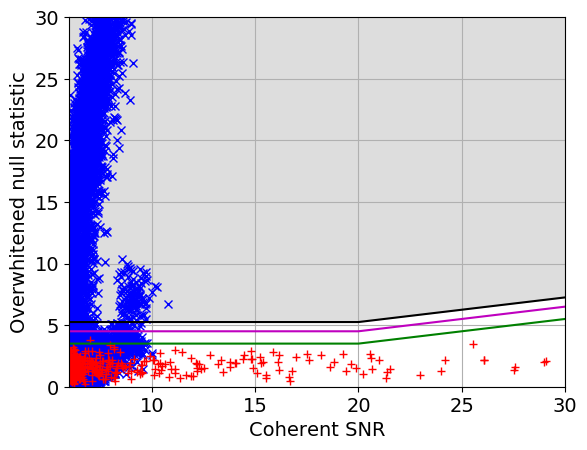
\includegraphics[width=0.8\linewidth]{GRB170817A_null_stat2_vs_snr_zoom.png}
\end{center}
\caption{\textbf{Null Stat Cut.} Here we plot the coherent SNR against the null SNR. The blue crosses are background triggers. The red pluses are signal injections. The black line is the veto line, with all triggers in the shaded region above the line being discarded. The green line indicates the expected SNR for optimally oriented injections. The magenta and cyan lines show 1 and 2 sigma errors on the green line. }
\label{fig:nullcut}
\end{figure}



\begin{itemize}
\item chi2 tests - Is this final? No coherent chi2 tests? Do we need to explain why we are no longer using coherent chi2 tests? 
\item Go through plot caption with Steve
\end{itemize}

\subsection{Reweighted SNR} \label{sec:reweighted snr}
After all the cuts have been made, the remaining triggers are then reweighted twice. First they are reweighted according to their coherent $\chi^2$ values, according to (\ref{chi2 reweigth}), then they are reweighted again according to their null SNR, according to (\ref{null reweight}).
\begin{equation}  \label{chi2 reweigth}
\rho_{\chi^2} = \begin{cases} \rho_\text{coh} & \mbox{if } \chi^2 \leq n_\text{dof} \\ \frac{\rho_\text{coh}}{\left( \frac{1}{2} \left[ 1 + \left( \frac{\chi^2}{n_\text{dof}} \right)^3 \right] \right)^{1/6} } & \mbox{if } \chi^2 > n_\text{dof}\end{cases}
\end{equation}  
\begin{equation} \label{null reweight}
\rho_\text{rw} = \begin{cases} \rho_{\chi^2} & \mbox{if } \rho_\text{null} \leq 4.25 \\ \frac{\rho_{\chi^2}}{ \rho_\text{null} -3.25} & \mbox{if } \rho_\text{null} > 4.25\end{cases}
\end{equation}
Note that this reweighting only down-weights triggers with a high $\chi^2$ or a high null SNR. The reweighting should not significantly alter the network SNR of a GW signal, but will reduce the SNR of noise. The reweighted SNR is the detection statistic used by PyGRB. 





\subsection{Event Significance} 
We use signal consistency checks to remove glitches from the trigger list, and we use the reweighted SNR to rank the surviving triggers in order of likelihood of being a real GW signal. The final step is to determine the significance of the surviving triggers, i.e. how often will we find glitches with a given reweighted SNR that have survived the signal consistency checks. We do this by calculating the false alarm probability (FAP) for each trigger. The FAP depends on the data quality at the time being analysed, as poor data quality leads to more high SNR glitches which makes finding a high SNR trigger less significant. For this reason, we must estimate the rate of high SNR glitches at the time of the GRB in order to determine the significance of a trigger. In this section we outline the process used to calculate event significance. 

As detector noise is not stationary, we calculate the FAP by using the data around the time of the GRB. If a GW is there, then it is assumed to be in the window starting five seconds before and ending one second after the GRB trigger time. This window would allow the detection of GWs from most GW models associated with short GRBs. We call this 6s window the \textit{on-source} window. The loudest\footnote{Here \textit{loudest} means highest reweighted SNR.} event, with the loudest template, in the on-source is taken as our trigger. 

To evaluate the p-value of this trigger, we analyse approximately one hour of data around the on-source\footnote{The amount of data used before and after the on-source varies depending on the data available. For example, sometimes a GRB will happen less than an hour before (after) an interferometer loses (acquires) lock.}, called the \textit{off-source} data. This data is assumed to not contain a GW signal. The off-source is divided up into as many 6s segments as possible, so that if we have $T_\text{off}$ seconds of data then we have $N=T_\text{off} / T_\text{on}$ segments, where $T_\text{on}$ is the length of the on-source. These segments are called the \textit{off-source-trials}. Using the same criteria as the for the on-source, we find the loudest trigger in each off-source-trial. As the off-source is assumed to only contain noise, the FAP of the on-source trigger is the fraction of off-trials that have a louder trigger than the on-source, i.e. the probability that noise would produce a trigger with a reweighted SNR louder than the on-source. 

This process alone is only capable of achieving a FAP of $10^{-3}$ [\textbf{Cite Andrew's paper}] as there is not enough off-trials to claim a lower FAP. This is low enough to reject a signal hypothesis, but not low enough to claim a detection, for which we require a FAP of less than $10^{-5}$ [\textbf{Cite Andrew again}]. One way to get around this would be to use a longer off-source, but as detector noise is not stationary, it is possible that this extra off-source data would have different properties to the time of the GRB. It would also significantly increase the computational time required to complete the analysis, as well as the amount of detector data required to analyse a GRB, meaning fewer GRBs are analysed.

To find a lower FAP, the off-source data from each detector is time-shifted relative to the other detectors in the network and the data is then reanalysed. The time-shifts are longer than the light travel time between the detectors in the network and also longer than the duration of a typical glitch (i.e. less than one second), so that triggers in the time shifted data are unlikely to appear coherently.  

There are two types of time shifting, called \textit{short slides} and \textit{long slides}. The two types of time slide is arise naturally from the fact that PyGRB analyses data in segments, typically of 128s. Time shifting the data within a segment is called \textit{short slides}. For example, in an HLV analysis the Hanford data is not shifted, the Livingston data is shifted in increments of 6s, and the Virgo data is shifted in increments of 12 seconds. This does not require the data to be matched filtered again, as the time shift happens after filtering. This means only the network statistics must be recomputed, making short slides computationally cheap but able to demonstrate a FAP as low as $10^{-4}$. \textit{Long slides} refers to when the segments themselves are shifted relative to one another. This requires the matched filtering to be redone, as the matched filter time series is not saved when moving to the next segment for analysis. This makes long slides much more computationally expensive than short slides. However, short slides can be done on top of the long slides, so that just 10 long slides are needed to show that a trigger has a FAP$<10^{-5}$.

It should be noted that our treatment of time slides assumes that each combination of time shifted data is statistically independent of the others. This is not true, as each combination of time shifted data is still the same data being analysed. For this reason, the FAP calculated from time slides is a lower limit on the true FAP. 


\subsection{Searching over a Sky Patch}
The sky position of GRBs cannot be determined exactly. The uncertainty in sky position depends on which satellites detected the GRB\footnote{See section \ref{sec:grb detectors} for details on the GRB detectors mentioned in this section.}. The BAT instrument on Swift can localise to within 1-4 arcminutes. This is a small enough uncertainty that the GW search can use a single sky point [\textbf{cite Andrew's paper?}]. Other GRB detectors cannot provide as precise localisation. The GBM on the Fermi satellite often provides a 3$\sigma$ confidence region with a roughly circular uncertainty with a radius of several degrees [\textbf{citation in Andrew's paper- maybe include this in grb det section}]. The IPN uses triangluation to determine sky position, so depending on the number of satellites in the IPN that make the detection, sky localisation can vary from under a square degree to thousands of square degrees. 

It is important to have approximately the correct sky position for a coherent search. If the sky position is incorrect, then the detector antenna patterns will be incorrect for the GRB, reducing the search sensitivity. More crucially, an incorrect sky position will cause the calculated time delays between detectors in the network to be wrong, making it impossible to correctly find coincident triggers between detectors. To overcome these issues, PyGRB searches over a grid of points that cover the uncertainty region provided by GRB detectors. 

The grid of points is constructed by filling the patch with concentric circles of points separated by $\delta a$, such that each ring has $2\pi n / \delta a$ points with $n=0$ being the central point of the patch. These concentric circles extend to cover the $3\sigma$ confidence region. The value of $\delta a$ depends on the depends on the timing uncertainty we are willing to accept. In practice, we use a timing uncertainty of $\delta t = 0.5$ms, which will limit the lost SNR to $<5\%$ [\textbf{cite andrew's paper}]. Searching over the sky grid is done after the computationally dominant step of matched filtering, so that searching over the sky grid does not significantly hurt analysis speed [\textbf{cite Andrew}].

In the two detector case, it is possible to search a reduced number of sky points without losing sensitivity. This is because there is a ring of sky points that give the same time delay between the two detectors. Searching different points on this ring would not change the time of arrival of a GW to the detectors, though it would change the antenna response factors. But the antenna response functions drop out of the formula for the coherent SNR (\ref{rhocoh}) in the two detector case\footnote{This is because in the two detector case, both the coherent and coincident SNR have four degrees of freedom. Thus, any observed amplitude and phase is consistent with an astrophysical signal.}. This means searching over different points on those sky rings would give exactly the same results. Thus, in the two detector case, we can analyse a greatly reduced set of sky points. Unfortunately, when we limit our search to looking for circularly polarised GWs, as discussed in section \ref{sec:circ pol}, then the antenna patterns again affect the detection statistic, and we must search over the sky grid.

\begin{figure} % Example of including images
\begin{center}
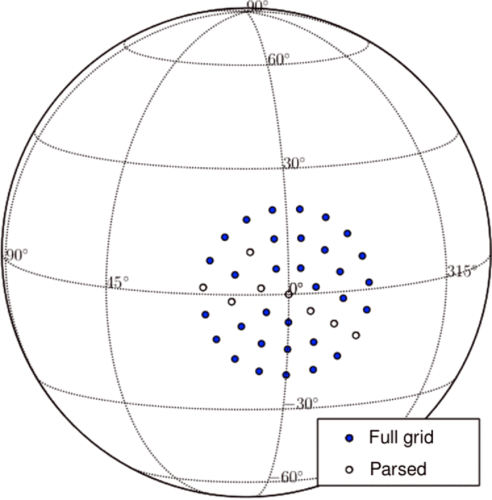
\includegraphics[width=0.6\linewidth]{skypatch.png}
\end{center}
\caption{\textbf{PyGRB Sky Grid.} Here we see an example of a full search grid used by PyGRB, indicated by the blue dots, and a reduced sky grid parsed by PyGRB in the case of a two detector search using the Hanford and Livingston detectors, the empty circles labeled 'parsed'. The parsed circles do not form a line due to the parsing routine, but this has no effect on analysis. \textbf{cite Andrew's paper}}
\label{fig:skypatch}
\end{figure}

\begin{itemize}
\item Is there a trials factor when searching over a sky grid? I assume there must be. Mention it. 
\end{itemize}


\subsection{Calculating Search Sensitivity} \label{sec:pygrb sensitivity}
It is useful to estimate the search sensitivity to GWs around the time of the analysed GRB. In the case that no GW is detected, this can be used to provide a lower limit on the distance of the source.  

To do this, we inject simulated signals into the off-source data and see if PyGRB can find them. The injected signals are CBC waveforms drawn from three populations: BNS mergers, NS-BH systems that have spins aligned with the angular momentum, and NS-BH systems with spins generically aligned. The injections are drawn from an astrophysically motivated distribution of distances, component masses and spins, and binary inclination. The NS mass distribution is a normal distribution with mean $1.4 \textup{M}_\odot$ and standard deviation of $0.2 \textup {M}_\odot$ [\textbf{refs in O2 GRB paper}] restricted to the $1 \textup{M}_\odot-3\textup {M}_\odot$ range [\textbf{refs in O2 GRB paper}]. The NS spins magnitude is restricted to be $\leq 0.4$, the fastest observed pulsar spin [\textbf{refs in O2 GRB paper}]. The BH masses are drawn from a normal distribution of mean $10 \textup{M}_\odot$ with standard deviation of 6$ \textup{M}_\odot$, restricted to the range $3 \textup{M}_\odot-15 \textup{M}_\odot$. The BH spin magnitudes are $\leq 0.98$, motivated by X-ray observations [\textbf{refs in O2 GRB paper}]. The injections are limited to have binary inclinations of $0^\circ-30^\circ$ or $150^\circ-180^\circ$, as the opening angle for a CBC powered GRB is expected to be less than $30^\circ$ [\textbf{cite BNS late time observations paper}]. 

We quantify the sensitivity of the search using the $50\%$ and $90\%$  exclusion distance. This is the distance at which $50\%$ and $90\%$ of the injected signals are recovered with a greater reweighted SNR than the most significant on-source trigger. 


\subsection{The PyGRB Workflow}
In figure \ref{fig:pygrb flowchart} you can see the PyGRB workflow. The workflow starts with two parallel branches: one for the injections runs (right branch) and the other for the background and on-source analysis (left branch). The non-injection branch is simpler. The template bank is split into many smaller template banks (typically $\sim 1500$). These are used by the inspiral jobs, which matched-filter the data, perform the consistency checks, and calculate the network SNR statistics. The results of each inspiral job are then compiled into by trig combiner and binned into off-source, on-source, or off-trial triggers. The off-trials are six six-second chunks of data which are each treated as a dummy on-source to assess whether the pipeline is behaving nominally before looking at the on-source results. Another file is produced which contains all triggers found in both the on-source and the off-source. Each of these is then \textit{clustered}, meaning only the loudest trigger with the loudest template in any 0.1 second window is kept. The clustered output is then used to calculate detection efficiencies and make plots before going into the results webpage. 

The injection jobs are similar but have a few extra steps. First the injections must be generated. At the moment this uses the same code (called \textit{inspinj}) as the all-sky search for black hole binaries. As we are only looking for binaries that could theoretically produce a GRB, we remove any injections that have the wrong masses or orientations.\footnote{The scripts that remove unsuitable injections are not included in the flowchart as they do not add much to the understanding of the workflow. In future, a script that produces just EM bright injections will be written to replace the ad hoc system we currently use.} The injections are then split into multiple jobs and combined with different parts of the split bank to be analysed by the inspiral code. These jobs can be run quickly by only searching the data with those templates that are expected to find the injections, rather than using the full template bank. The \textit{injfinder} code analyses the output of the injection inspiral jobs to determine which injections were found and which were not. The \textit{injcombiner} job then bins the injections into the appropriate off-trial or the on-source. The injcombiner output is used to calculate injection detection efficiencies and make plots, which are then used in the results webpage. 

\begin{sidewaysfigure} % Example of including images
\begin{center}
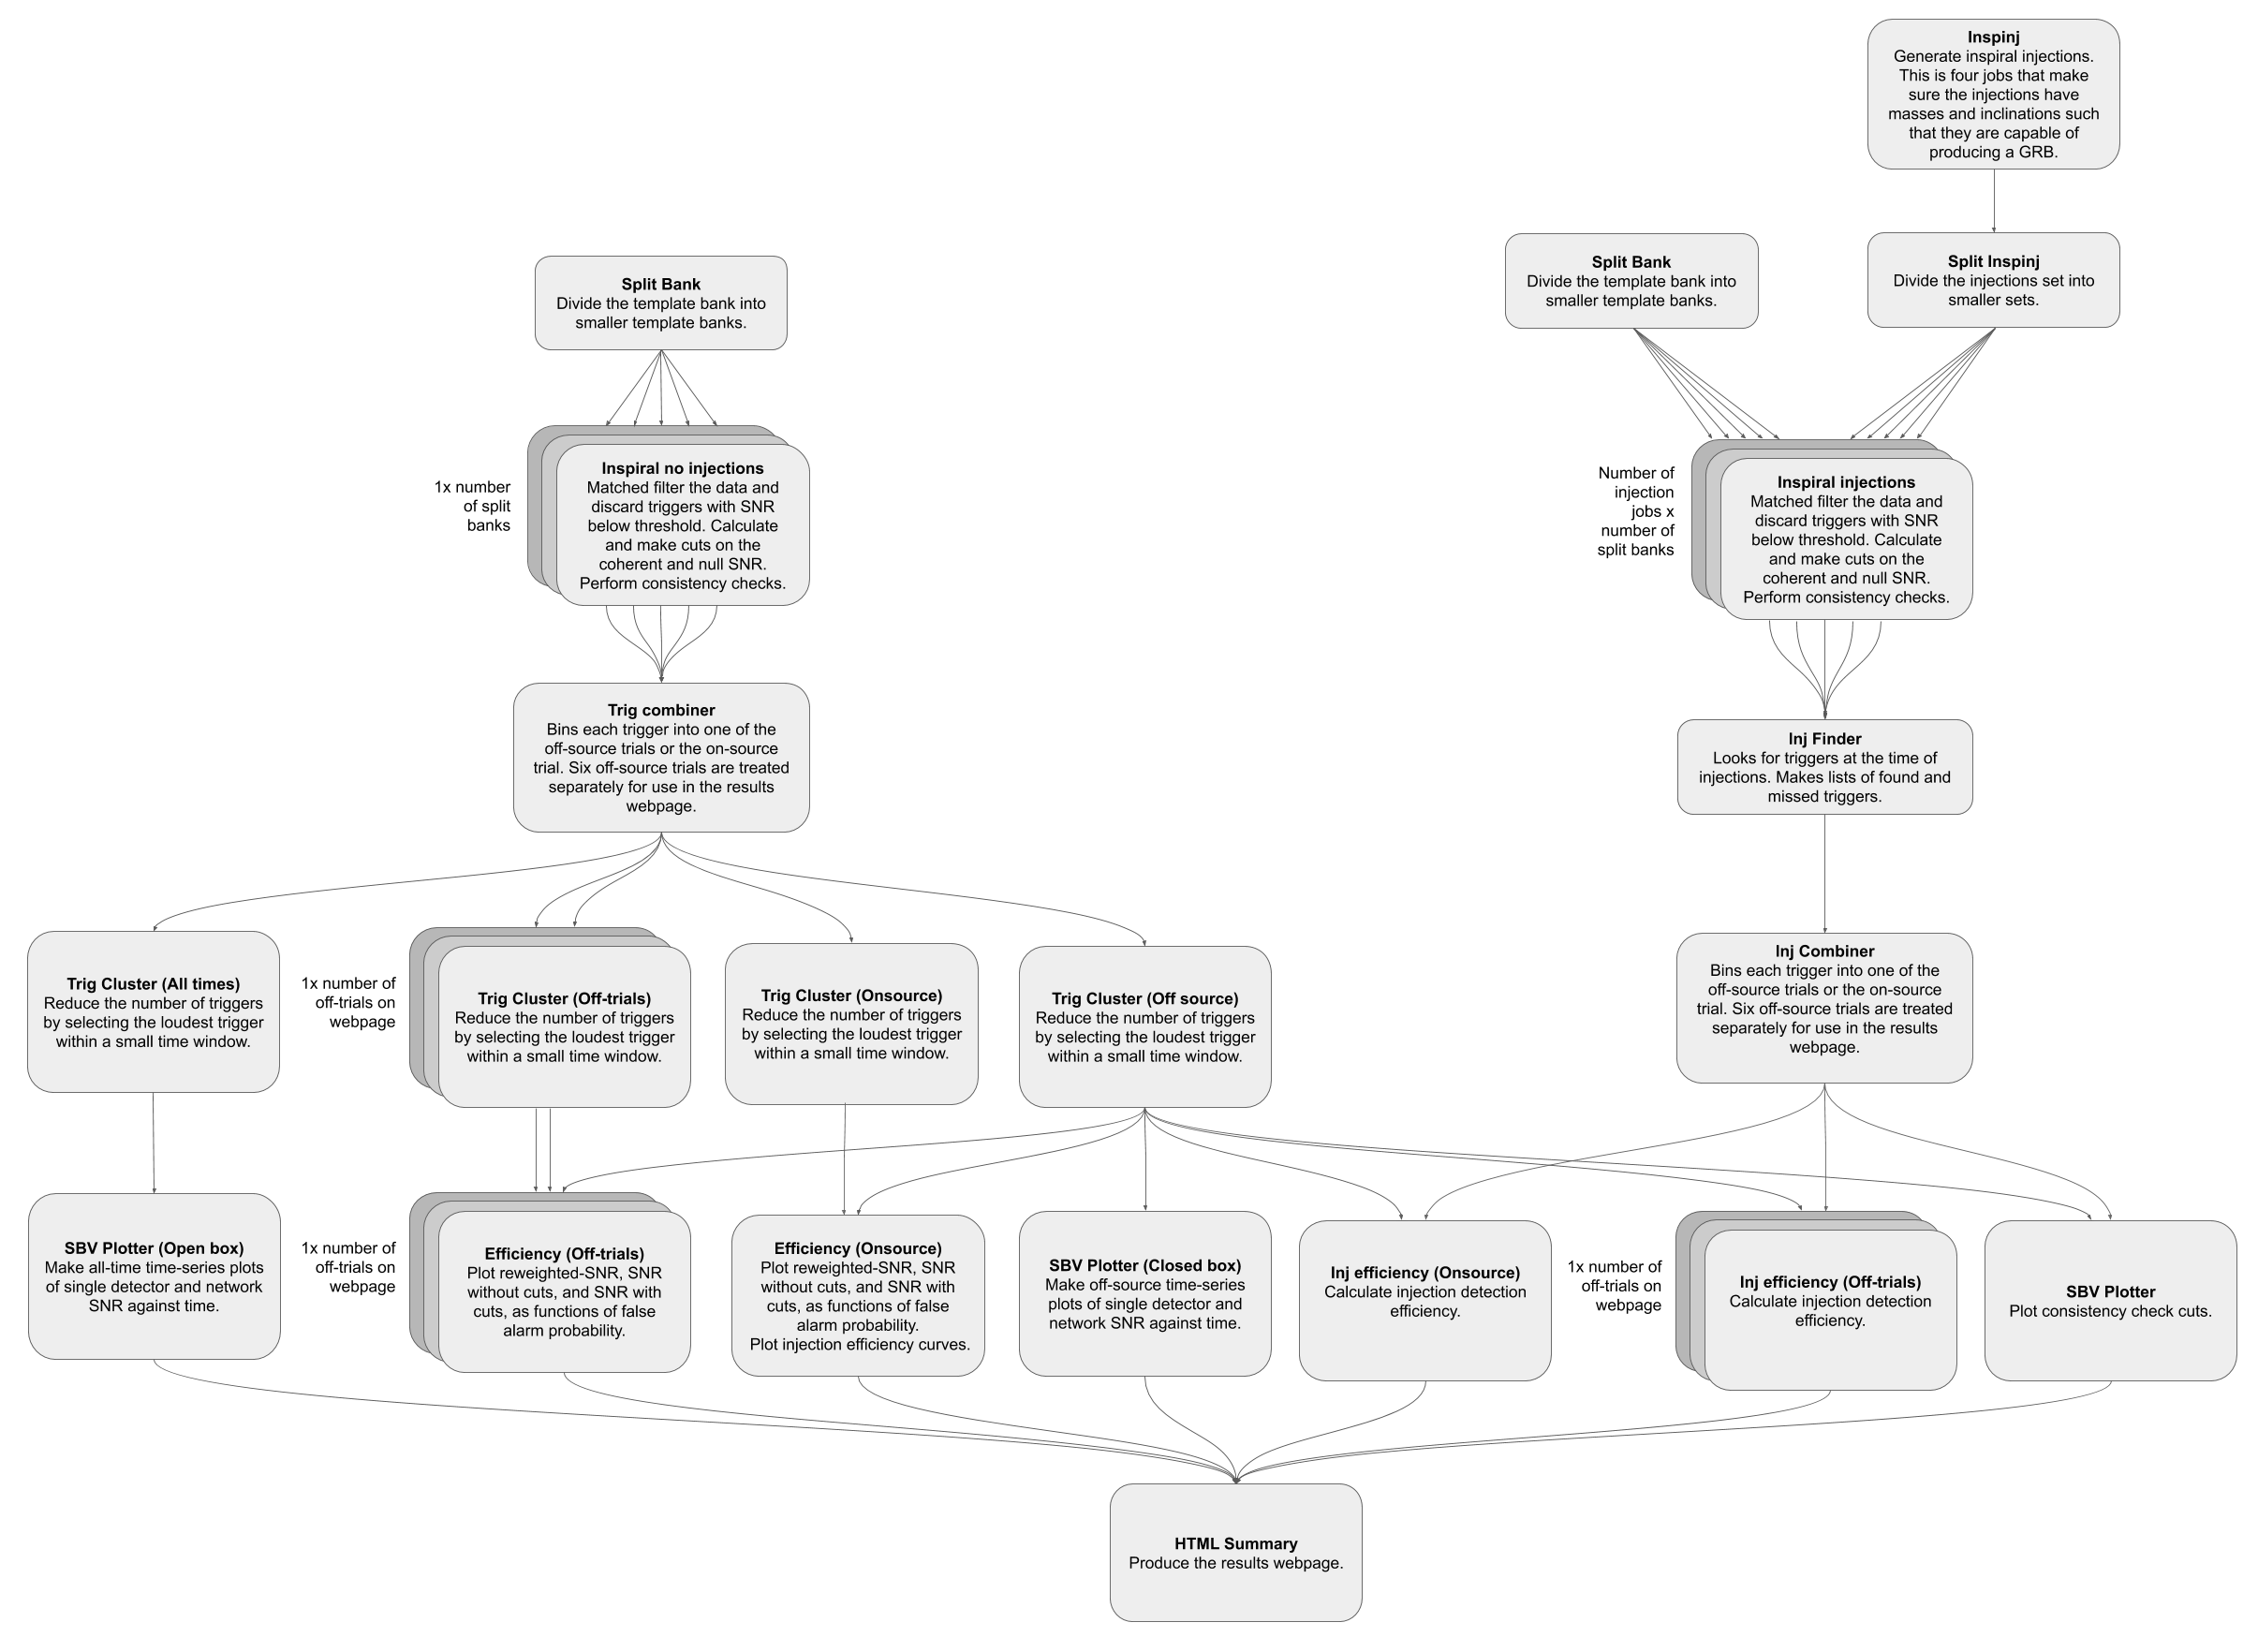
\includegraphics[width=1.0\linewidth]{pygrb_flowchart.png}
\end{center}
\caption{\textbf{PyGRB Workflow.} The workflow starts in two parallel branches, one that runs the injections jobs, and one that analyses the background and onsource. }
\label{fig:pygrb flowchart}
\end{sidewaysfigure}

\section{O2 PyGRB Search} \label{sec:pygrb o2 results}
From November 2016 to August 2017, the Advanced LIGO detectors undertook their second observing run, O2, with the Advanced Virgo detector joining on August 1st 2017. PyGRB was used to search for GW signals associated with short and ambiguous duration GRBs detected during O2. The results of the search were reported in [\textbf{cite O2 GRB paper}], but we will outline the key findings here. We begin with a brief discussion of the GRB sample that was analysed before moving on to the results of the search.

\subsection{GRB sample}
The GRBs analysed were those detected by Swift BAT, Fermi GBM, or the IPN (see section \ref{sec:grb detectors} for more details on these). There were in total 242 bursts detected by Swift and Fermi, and 52 detected by the IPN, with many GRBs appearing in both catalogues. Only short GRBs ($T_{90}<2s$) and ambiguous GRBs ($2s<T_{90}<4s$) were analysed using PyGRB, as long GRBs are not expected to have a CBC progenitor (as discussed in chapter \ref{chap:GRBs}). At least 1664s of data is required for PyGRB to correctly estimate the background. Any detector that does not have this much data available around the time of a GRB is not used for the analysis, and if no detectors have sufficient data available then PyGRB will not analyse that GRB. Removing the GRBs for which there was insufficient data left 42 short/ambiguous GRBs that could be analysed by PyGRB.


\subsection{Results}
The analysis found one GW signal, GW 170817. It was associated with GRB 170817A and had been previously reported [\textbf{cite BNS paper}]. The p-value for this event is $\leq 9.38 \times 10^{-6}$ and the coherent SNR is 31.26 [\textbf{cite O2 GRB}]. No other GWs were detected in conjunction with any other GRBs. Apart from GW 170817, there were six GRBs with a p-value of less than 0.1. These candidate events had further data quality checks, which found no clear noise source that could explain the triggers. They were then analysed using lalInference [\textbf{cite Veitch like in GRB paper}], a coherent Bayesian parameter estimation pipeline, to determine if there could be a subthreshold signal in the data or if it was more likely to be background noise. No evidence was found of a subthreshold signal. 

In figure \ref{fig:pvalue} we have plotted the p-value for the remaining 41 GRBs analysed after the removal GW 170817 from the sample. For GRBs with no trigger in the on-source window, we provide upper and lower limits on the p-value. The upper limit is a p-value of 1. The lower limit is the fraction of off-source trials that also had no trigger. The distribution lays within the $2\sigma$ range, shown by the upper and lower dotted lines. The population consistency with a no-signal hypothesis was calculated using the weighted binomial test outlined in [\textbf{cite abadie et al}]. This test considers the lowest $5\%$ of p-values in the population, weighted by their prior probability of detection based on the time and sky position of the GRB. This analysis did not include GW 170817 as it is a confirmed detection. The combined p-value for the search is 0.3. Thus we find no significant evidence for a population of subthreshold signals.  

\begin{figure}
\begin{center}
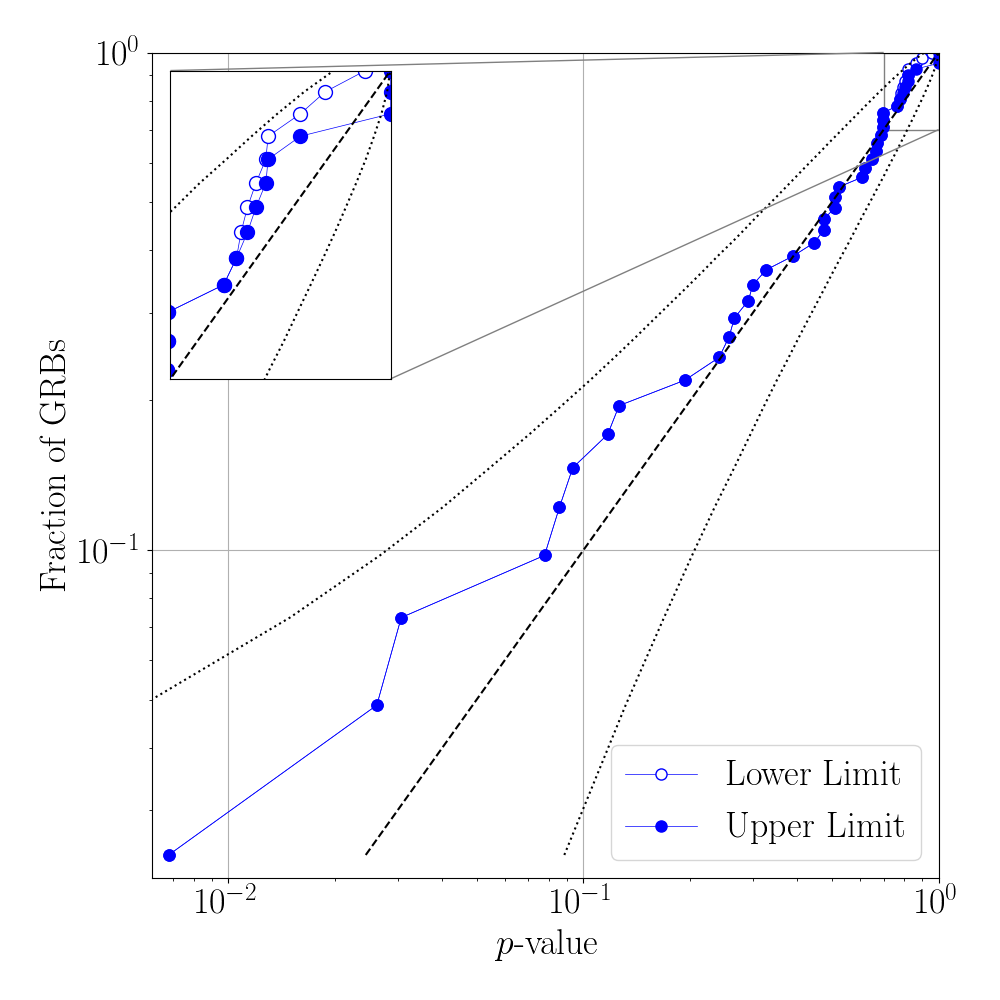
\includegraphics[width=0.8\linewidth]{pygrb_pvalue.png}
\end{center}
\caption{\textbf{P-value for each GRB.} This is the p-value distribution for the 41 GRBs other than GRB 170817A. The GRBs with no trigger in the onsource window have upper and lower limits on the p-value. The upper limit is a p-value of 1. The lower limit is the fraction of offsource trials that also had no trigger. The distribution lays within the $2\sigma$ range, shown by the upper and lower dotted lines.  }
\label{fig:pvalue}
\end{figure}

As GRB 170817A is known to have originated in the galaxy NGC 4993 [\textbf{cite paper}], the distance to this GRB is approximately 43Mpc. For the other GRBs in our sample we calculated the $90\%$ exclusion distance. This is the distance at which $90\%$ of the signal injections are recovered with a greater coherent SNR than the loudest trigger in the on-source. The $90\%$ exclusion distances are plotted in figure \ref{fig:ex dist}. The median $90\%$ exclusion distance for the BNS waveform is 80 Mpc, for an NS-BH waveform with generic spin is 105 Mpc, and for NS-BH with aligned spin is 144 Mpc. These values are slightly lower than in O1, which were 90 Mpc, 139 Mpc, and 150 Mpc respectively, though this seems to just be due to a statistical fluctuation as we analysed a relatively small number of GRBs. There is a summary of the information about each GRB analysed by PyGRB in table \ref{tab:grbs}. This table includes teh $90\%$ exclusion distance for each waveform type for each GRB.

\begin{figure}
\begin{center}
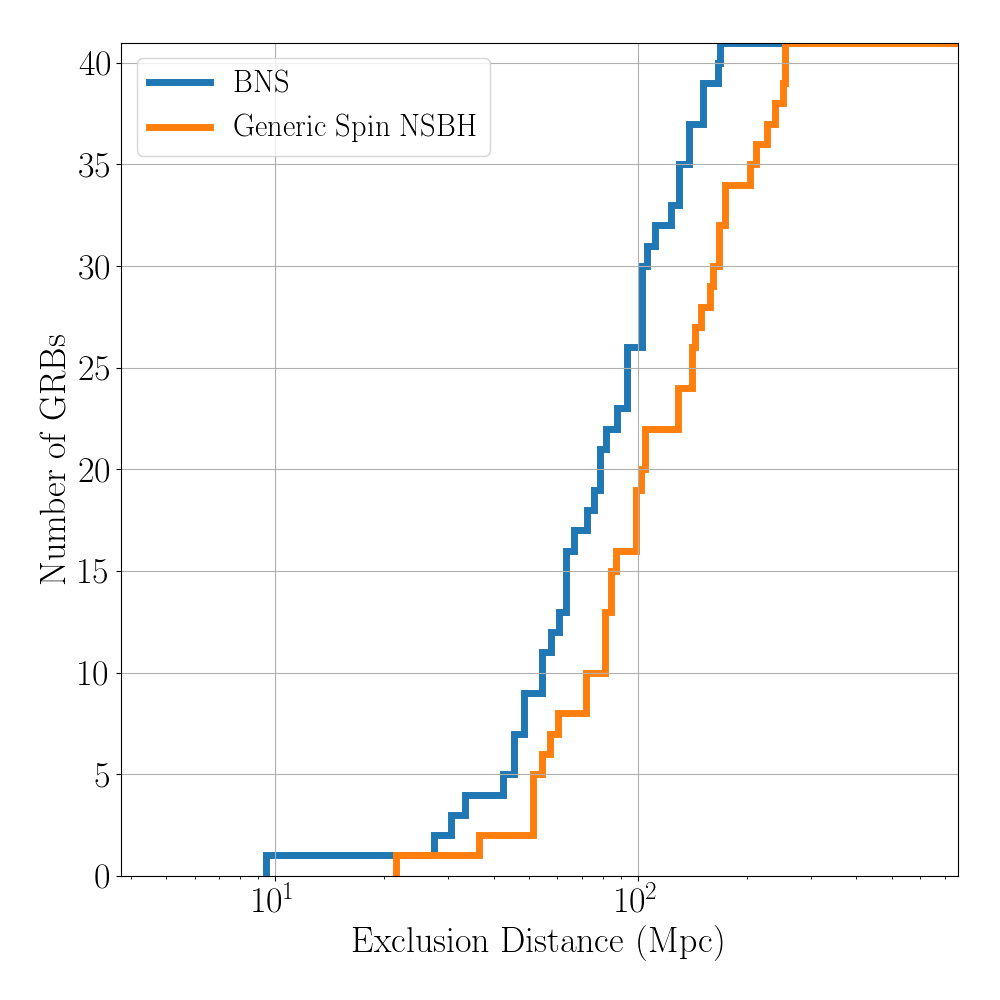
\includegraphics[width=0.8\linewidth]{pygrb_exclusion_distance.png}
\end{center}
\caption{\textbf{Cumulative exclusion distance.} This is the cumulative $90\%$ exclusion distance for every GRB analysed by PyGRB except GRB170817A.  The $90\%$ exclusion distance is the distance at which $90\%$ of injected simulated signals are recovered with a greater coherent SNR than the loudest trigger in the onsource. }
\label{fig:ex dist}
\end{figure}


\begin{landscape}
\begin{tabular}{l c  c  c  c  c  c  c  c c |}
\hline
 GRB & UTC time & ra & dec & satellite & network & BNS & NSBH generic spin & NSBH aligned spin \\
\hline
161217128 & 03:03:46  & $14^{\mathrm{h}}26^{\mathrm{m}}31^{\mathrm{s}}$ & $51^{\circ}58'$ &  Fermi   & H1L1   & 65  & 85  & 122 \\
170112A   & 02:01:59  & $01^{\mathrm{h}}00^{\mathrm{m}}55^{\mathrm{s}}$ & $-17^{\circ}13'$ & Swift   & H1L1   & 83  & 106 & 144 \\
170121133 & 03:10:52  & $16^{\mathrm{h}}07^{\mathrm{m}}58^{\mathrm{s}}$ & $13^{\circ}48'$ &  Fermi   & H1L1   & 96  & 142 & 172 \\
170125022 & 00:31:14  & $17^{\mathrm{h}}36^{\mathrm{m}}34^{\mathrm{s}}$ & $28^{\circ}34'$ &  Fermi   & H1     & 46  & 52  & 57 \\
170127067 & 01:35:48  & $22^{\mathrm{h}}37^{\mathrm{m}}19^{\mathrm{s}}$ & $-63^{\circ}56'$ & Fermi   & H1L1   & 76  & 129 & 141 \\
170203486 & 11:40:26  & $16^{\mathrm{h}}20^{\mathrm{m}}22^{\mathrm{s}}$ & $-00^{\circ}30'$ & Fermi   & H1L1   & 66  & 99  & 119 \\
170219002 & 00:03:07  & $03^{\mathrm{h}}39^{\mathrm{m}}22^{\mathrm{s}}$ & $50^{\circ}04'$ &  Fermi   & H1L1   & 171 & 251 & 304 \\
170302166 & 03:58:24  & $10^{\mathrm{h}}17^{\mathrm{m}}00^{\mathrm{s}}$ & $29^{\circ}23'$ &  Fermi   & H1L1   & 107 & 175 & 206 \\
170305256 & 06:09:07  & $02^{\mathrm{h}}34^{\mathrm{m}}38^{\mathrm{s}}$ & $12^{\circ}05'$ &  Fermi   & L1     & 48  & 73  & 82 \\
170325331 & 07:56:58  & $08^{\mathrm{h}}29^{\mathrm{m}}55^{\mathrm{s}}$ & $20^{\circ}31'$ &  Fermi   & H1L1   & 73  & 88  & 125 \\
170428A   & 09:13:42  & $22^{\mathrm{h}}00^{\mathrm{m}}12^{\mathrm{s}}$ & $26^{\circ}54'$ &  Swift   & H1L1   & 105 & 167 & 178 \\
170506169 & 04:02:48  & $07^{\mathrm{h}}29^{\mathrm{m}}02^{\mathrm{s}}$ & $51^{\circ}52'$ &  Fermi   & H1L1   & 103 & 174 & 149 \\
170614505 & 12:06:39  & $20^{\mathrm{h}}43^{\mathrm{m}}58^{\mathrm{s}}$ & $-37^{\circ}54'$ & Fermi   & H1     & 9   & 22  & 0 \\
170709334 & 08:00:24  & $20^{\mathrm{h}}40^{\mathrm{m}}10^{\mathrm{s}}$ & $02^{\circ}12'$ &  Fermi   & L1     & 139 & 228 & 255 \\
170726249 & 05:58:15  & $11^{\mathrm{h}}05^{\mathrm{m}}41^{\mathrm{s}}$ & $-34^{\circ}00'$ & Fermi   & H1L1   & 124 & 152 & 207 \\
170802638 & 15:18:25  & $03^{\mathrm{h}}29^{\mathrm{m}}12^{\mathrm{s}}$ & $-39^{\circ}12'$ & Fermi   & H1L1V1 & 45  & 62  & 72 \\
170805B   & 14:18:49  & $09^{\mathrm{h}}42^{\mathrm{m}}31^{\mathrm{s}}$ & $69^{\circ}54'$ &  IPN     & H1L1V1 & 132 & 163 & 218 \\
170808065 & 01:34:09  & $00^{\mathrm{h}}13^{\mathrm{m}}12^{\mathrm{s}}$ & $62^{\circ}18'$ &  Fermi   & L1V1   & 58  & 83  & 87 \\
170817908 & 21:47:34  & $05^{\mathrm{h}}32^{\mathrm{m}}07^{\mathrm{s}}$ & $50^{\circ}04'$ &  Fermi   & H1V1   & 35  & 51  & 63 \\
161210524 & 12:33:54  & $18^{\mathrm{h}}52^{\mathrm{m}}29^{\mathrm{s}}$ & $63^{\circ}03'$ &  Fermi   & H1L1   & 61  & 72  & 112 \\
161212652 & 15:38:59  & $01^{\mathrm{h}}39^{\mathrm{m}}36^{\mathrm{s}}$ & $68^{\circ}12'$ &  Fermi   & H1     & 49  & 59  & 60 \\
\end{tabular}
\end{landscape}

\begin{landscape}
\begin{tabular}{ccccccccc}
\hline
 GRB & UTC time & ra & dec & satellite & network & BNS & NSBH generic spin & NSBH aligned spin \\
\hline
170111815 & 19:34:01  & $18^{\mathrm{h}}03^{\mathrm{m}}31^{\mathrm{s}}$ & $63^{\circ}42'$ &  Fermi   & H1     & 95  & 160 & 198 \\
170121067 & 01:36:54  & $00^{\mathrm{h}}12^{\mathrm{m}}07^{\mathrm{s}}$ & $-75^{\circ}37'$ & Fermi   & H1L1   & 79  & 105 & 144 \\
170124528 & 12:40:29  & $00^{\mathrm{h}}43^{\mathrm{m}}24^{\mathrm{s}}$ & $11^{\circ}01'$ &  Fermi  & H1      & 65  & 101 & 116 \\
170125102 & 02:27:10  & $23^{\mathrm{h}}57^{\mathrm{m}}38^{\mathrm{s}}$ & $-38^{\circ}13'$ & Fermi   & H1     & 30  & 39  & 63 \\
170127B   & 15:13:29  & $01^{\mathrm{h}}19^{\mathrm{m}}58^{\mathrm{s}}$ & $-30^{\circ}20'$ & Swift   & H1     & 113 & 169 & 197 \\
170206A   & 10:51:58  & $14^{\mathrm{h}}12^{\mathrm{m}}43^{\mathrm{s}}$ & $12^{\circ}34'$ &  IPN   & H1L1     & 151 & 254 & 264 \\
170222A   & 05:00:59  & $19^{\mathrm{h}}31^{\mathrm{m}}53^{\mathrm{s}}$ & $28^{\circ}04'$ &  IPN   & H1L1     & 80  & 86  & 112 \\
170304003 & 00:04:26  & $22^{\mathrm{h}}02^{\mathrm{m}}00^{\mathrm{s}}$ & $-73^{\circ}45'$ & Fermi   & H1L1   & 105 & 143 & 178 \\
170318B   & 15:27:53  & $18^{\mathrm{h}}57^{\mathrm{m}}10^{\mathrm{s}}$ & $06^{\circ}19'$ &  Swift   & H1L1   & 152 & 254 & 281 \\
170403583 & 13:59:18  & $17^{\mathrm{h}}48^{\mathrm{m}}19^{\mathrm{s}}$ & $14^{\circ}31'$ &  Fermi   & H1L1   & 166 & 240 & 261 \\
170430204 & 04:54:20  & $01^{\mathrm{h}}35^{\mathrm{m}}26^{\mathrm{s}}$ & $30^{\circ}07'$ &  Fermi   & H1     & 32  & 54  & 81 \\
170604603 & 14:28:05  & $22^{\mathrm{h}}41^{\mathrm{m}}36^{\mathrm{s}}$ & $40^{\circ}42'$ &  Fermi   & L1     & 131 & 204 & 237 \\
170708046 & 01:06:11  & $22^{\mathrm{h}}13^{\mathrm{m}}00^{\mathrm{s}}$ & $25^{\circ}37'$ &  Fermi   & L1     & 57  & 105 & 103 \\
170723882 & 21:10:18  & $14^{\mathrm{h}}10^{\mathrm{m}}19^{\mathrm{s}}$ & $39^{\circ}49'$ &  Fermi   & H1L1   & 95  & 83  & 179 \\
170728A   & 06:53:29  & $03^{\mathrm{h}}55^{\mathrm{m}}36^{\mathrm{s}}$ & $12^{\circ}09'$ &  Swift   & H1L1   & 89  & 129 & 163 \\
170803172 & 04:07:16  & $05^{\mathrm{h}}06^{\mathrm{m}}00^{\mathrm{s}}$ & $24^{\circ}00'$ &  Fermi   & H1L1V1 & 56  & 83  & 105 \\
170803B   & 22:00:32  & $00^{\mathrm{h}}56^{\mathrm{m}}53^{\mathrm{s}}$ & $06^{\circ}34'$ &  IPN   & L1       & 140 & 215 & 234 \\
170805A   & 14:38:11  & $17^{\mathrm{h}}55^{\mathrm{m}}12^{\mathrm{s}}$ & $-23^{\circ}30'$ & IPN   & H1L1V1   & 69  & 100 & 114 \\
170817A   & 12:41:06  & $13^{\mathrm{h}}09^{\mathrm{m}}36^{\mathrm{s}}$ & $-23^{\circ}24'$ & Fermi   & H1L1V1 & 0   & 0   & 41 \\
170818137 & 03:17:20  & $19^{\mathrm{h}}48^{\mathrm{m}}53^{\mathrm{s}}$ & $06^{\circ}21'$ &  Fermi   & H1L1   & 103 & 146 & 169 \\
170816599 & 14:23:04  & $23^{\mathrm{h}}25^{\mathrm{m}}36^{\mathrm{s}}$ & $19^{\circ}06'$ &  Fermi   & H1V1   & 46  & 56  & 73 \\ 
\end{tabular}
\label{tab:grbs}
\end{landscape}

\subsection{Rates}

\chapter{Improvements to PyGRB} \label{sec:pygrb improvements}
In the previous chapter we discussed the PyGRB pipeline as it was used in the second LIGO observing run. The code is now about 10 years old, and in that time new software tools have become available that could speed up the and improve the analysis. In particular, there is the PyCBC software package [\textbf{cite pycbc paper}], which has highly optimised tools for performing a matched filter search. For this reason, PyGRB is being rewritten to be fully implemented into PyCBC. In this chapter we will begin by discussing the reasons why this change was necessary before seeing what changes have already been made and the improvements they provide. We will then end this chapter by looking forward at the changes that need to happen for the PyGRB rewrite to be used in a GW search.


\section{Reasons to Rewrite the Pipeline}
The primary reason for rewriting the pipeline is to make use of the faster and more efficient matched filtering software that PyCBC can provide. Developments in the all-sky search have drastically sped up matched filtering in recent years, to the point where PyGRB was becoming noticeably slow by comparison. Apart from being a waste of computer time, this also limits the science that can be done with PyGRB. The medium latency PyGRB search aims to provide a preliminary analysis of a GRB within a day. As kilonovas following short GRBs fade on a timescale of hours, this delay can mean missing vital data from the time immediately after merger. With the new code, we expect to be able to perform a preliminary analysis (with minimal injections and no timeslides) within a couple of hours. It also limits the size of the sky patch that can be searched over in a reasonable amount of time. There were four short GRBs in O2 that were not well localised enough for PyGRB to analyse,\footnote{These were all IPN detections, which can have poor localisation depending on which detectors in the network see the GRB (see section \ref{sec:grb detectors}).} which could have been with faster, more efficient code. And finally, it limits the number of timeslides that can be performed, and consequently the false alarm probability that can be achieved. 

There are two bottlenecks in the PyGRB workflow. The first is the matched filtering, where using the PyCBC matched filtering engine can lead to significant speed up. The other is in post-processing, which can be sped up significantly by using a modern file format.\footnote{The old code used xml files, which are significantly slower than the hdf5 files used by the new code.} The post-processing also frequently exceeds the memory allowance on computing clusters, which requires the job to be manually halted and rerun with the post-processing split into smaller jobs. As PyGRB deals with far fewer triggers (and so should use less memory) than the all-sky search, this should not be a problem. Using tools developed for the all-sky search can fix this. 

Faster code is not the only reason for integrating PyGRB into PyCBC. New tools have been made for the all-sky search will become available to the targeted search\footnote{These will be discussed in more detail in section \ref{sec:pygrb changes}} as well as any future improvements. It will also allow for techniques developed for the targeted search to be adopted by the all-sky search. For example, the all-sky search could adopt a hierarchical approach where coherent follow-up is performed on the sky patch around sub-threshold triggers, improving the false alarm rate.  

\begin{itemize}
\item Speed and memory usage comparisons between all sky and targeted search
\end{itemize}

\section{New Code Changes} \label{sec:pygrb changes}
In the previous section we discussed the reasons why rewriting PyGRB was necessary. In this section we will see how the code has changed. The rewrite was not simply a case of carrying out the same analysis with a faster matched filtering engine. The new analysis is qualitatively different from the old code. We will look at is the new consistency checks, we will see some of the tools used in the all-sky search that are now available to the targeted search, we will discuss the new detection statistic used, and finally we will see how much faster the new analysis is than the old. 

\subsection{Consistency Checks} \label{sec:new chisq}
\begin{itemize}
\item Quick summary of old chisq and point to section in previous chapter
\item No coherent chi2 any more
\item Coherent chisq just washes out the chisq
\item Use single ifo chisq in combination 
\end{itemize}


\subsection{New Data Analysis Tools}
\begin{itemize}
\item Denty bins
\item Autogating
\item And any future developments
\end{itemize}



\subsection{Detection Statistic}
\begin{itemize}
\item Re-optimised the cuts and reweighted snr
\end{itemize}

\subsection{Speed Gains}
\begin{itemize}
\item Single sky point analysis with no face on/off analysis
\item Speed gains from optimised ffts
\item Compare analysis speed for 170817 and a swift GRB
\item Show results are comparable 
\item Ran on a single sky point in 2 hours 
\end{itemize}

\section{Future Plans}
\begin{itemize}
\item Sky grid
\item Time slides
\item More detectors strengthens the case for coherent search
\item Hierarchical search, using coincident search to find location 
\item Include astrophysical priors in the detection statistic
\item Expected rates (from structured jet paper, one in 20 BNS mergers detected with GWs will have a GRB counterpart)
\item use p astro
\end{itemize}


\chapter{A Search for Unmodelled Gravitaional Wave Signals using Machine Learning} \label{chap: mva}

The Laser Interferometer Gravitational Wave Observatory (LIGO) and Virgo collaborations operate ground-based gravitational wave (GW) detectors. They have detected signals of astrophysical origin, including the merger of a binary neutron star (BNS) system and multiple binary black hole (BBH) merger signals. As these sources have a known signal morphology, they can be found using a highly sensitive matched-filter search, as discussed in chapter \ref{CBC search}. Some of the most interesting potential sources of GWs, such as core collapse supernova, do not have a known waveform morphology and so a matched filter search is not possible. For this reason, it is important to develop unmodelled searches as well. Unmodelled searches look for coherence between the data streams of multiple interferometers. We will consider the case of a burst search where the sky position of the candidate source is known. This allows us to calculate the relative time of arrival and the relative signal power in each detector.

In this chapter, we will first discuss how an existing targeted burst search, called \textit{X-pipeline}, searches for gravitational wave bursts (GWBs). We will then see how we can improve this pipeline by using \textit{multivariate analysis} (MVA) to apply rank candidate GW events.  

\section{X-pipeline} \label{xtriggers}
\xp is a targeted search for GWBs. It uses the sky location of an astrophysical event, such as a GRB, as reported by EM astronomers. The sky location is used to time-shift the data from each GW detector so that the signal arrives simultaneously in each data stream. \xp then coherently combines the data streams of the individual detectors to make:
\begin{itemize}
\item \textit{Signal streams}, which increase the power of a GW signals relative to noise.
\item \textit{Null streams}, which reduce the power of true GW signals but not noise.
\end{itemize}
\textit{Triggers} are groups of neighbouring pixels that are above threshold in a time-frequency map of a signal stream (see fig.\ref{fig:tfmap}). \xp  then cuts triggers based on correlations of the various signal and null data streams (see figure \ref{fig:xcuts}). The position of these cuts is set to give the best detection efficiency at a fixed false alarm rate, determined using a subset of the triggers that are used for tuning. For the MVA pipeline, the position of these cuts is instead set by a machine learning algorithm (as we will see in \ref{ML}).

\begin{figure} % Example of including images
\begin{center}
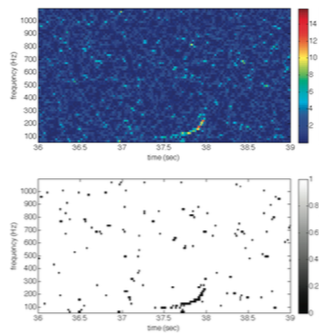
\includegraphics[width=0.8\linewidth]{xpipelineTFmap.png}
\end{center}
\caption{\textbf{Xpipeline Time-Frequency Map} This figure shows a time-frequency map from Xpipeline for a $1.4-10 M_\odot$ NSBH merger. The top figure shows the $E_+$ energy and the bottom figure shows the top 1\% of pixels. [\textbf{cite xp paper}] } 
\label{fig:tfmap}
\end{figure}

\begin{figure} % Example of including images
\begin{center}
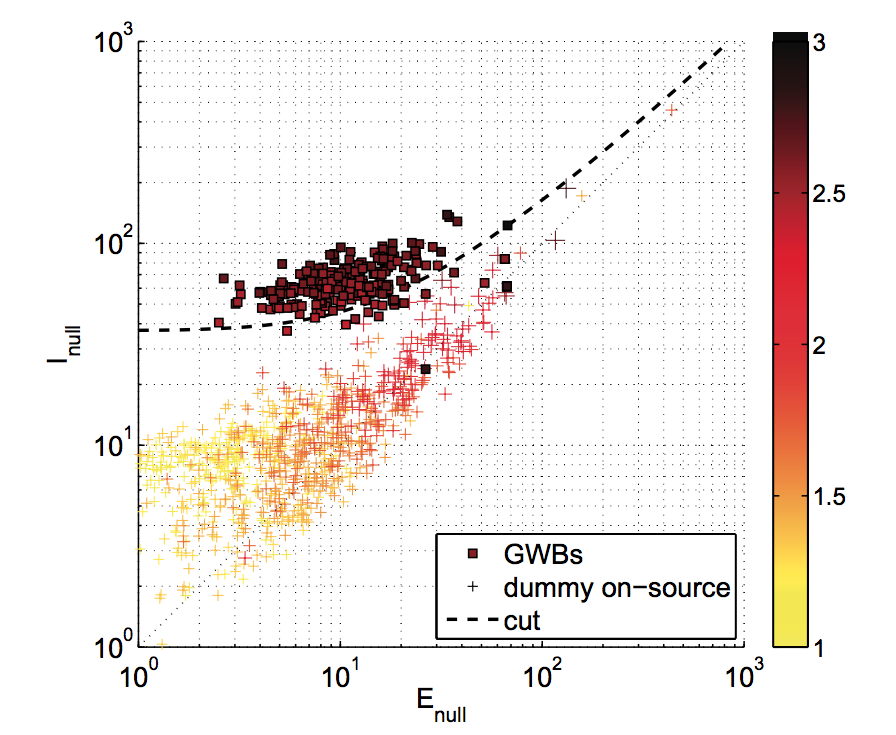
\includegraphics[width=0.8\linewidth]{xpipeline_cut.png}
\end{center}
\caption{\textbf{Xpipeline Cut} This figure shows Xpipeline making a cut to eliminate many spurious signals. } %\cite{xpipeline_paper}
\label{fig:xcuts}
\end{figure}

In this section, we will derive two of the coherent data-streams generated by \xp, as illustrative examples. The first is a signal-stream, called the \textit{standard likelihood}. We will then use the standard likelihood to create a null-stream. 

\subsection{Burst Search Background}
Suppose we have a network of $D$ detectors. A gravitational wave, described by $h_+(t)$ and $h_\times (t)$, passes through the Earth from direction $\hat{\Omega}$. We describe the sensitivity of detector $\alpha \in \{1,...,D \}$ to the plus and cross polarizations using the \emph{Antenna Response Functions}, denoted $\Fp (\hat{\Omega})$ and $\Fx(\hat{\Omega})$. The position of detector $\alpha$ is denoted by $\textbf{r}_\alpha$ and the noise in this detector is given by $n_\alpha (t)$. The detector output $d_\alpha (t)$ is then given by
\begin{equation} \label{det_output}
d_\alpha (t + \Delta t_\alpha (\hat{\Omega})) = \Fp (\hat{\Omega}) h_+ (t) + \Fx (\hat{\Omega}) h_\times (t) + n_\alpha (t + \Delta t_\alpha (\hat{\Omega})) \fs
\end{equation}   
Here $\Delta t_\alpha$ is the time taken for the GW to reach the detector from some arbitrary reference point\footnote{The center of the Earth is a fairly intuitive choice for a worldwide detector network.} $\textbf{r}_0$

\begin{equation}
\Delta t_\alpha (\hat{\Omega})=\frac{1}{c}(\textbf{r}_0-\textbf{r}_\alpha)\cdot\hat{\Omega} \fs
\end{equation}
%To understand why this time delay only appears in the noise of the above equation, think of the GW passing through the point $\textbf{r}_0$ at time $t$. The antenna response functions and the GWs waveform will not change between $\textbf{r}_0$ and $\textbf{r}_\alpha$, so the first two terms in \ref{det_output} are fixed. But it will take $\Delta t_\alpha$ to reach the detector, and so we must consider the noise in the detector at that moment to correctly determine the detectors output. 
From now on we will suppress explicit mention of the reference point $\textbf{r}_0$ or the time delay $\Delta t_\alpha$ on the understanding that detector outputs need to be time-shifted by an appropriate amount. 

In reality, detector outputs are not continuous but sampled discretely. The discrete Fourier transform $\tilde{x}[k]$ of the time series $x[j]$, and its inverse, are given by
\begin{equation}
\tilde{x}[k]=\sum^{N-1}_{j=0} x[j] e^{-i 2\pi jk/N}, \hspace{20pt}x[i]=\frac{1}{N}\sum^{N-1}_{j=0} \tilde{x}[k] e^{i2 \pi jk/N} \fs
\end{equation}
For sampling rate is $f_s$ and $N$ data points in the time domain, we convert continuous to discrete notation by using
\begin{equation}
x(t)\rightarrow x[j]
\end{equation} 
\begin{equation}
\tilde{x}(f)\rightarrow f^{-1} \tilde{x}[k]
\end{equation} 
\begin{equation}
\int dt \rightarrow f_s^{-1}\sum_j
\end{equation} 
\begin{equation}
\int df \rightarrow f_s N^{-1} \sum_k
\end{equation} 
\begin{equation}
\delta(t-t')\rightarrow f_s \delta_{jj'}
\end{equation}
\begin{equation}
\delta(f-f')\rightarrow N f_s^{-1}\delta_{kk'} \fs
\end{equation}  
For example, the one-sided noise spectral density for a detector with noise $n(t)$ can be written in continuous form as
\begin{equation}
\langle  \tilde{n}^* (f) \tilde{n} (f') \rangle = \delta (f-f') \frac{1}{2} S_n (f)
\end{equation}
where the angle brackets indicate an average over the noise. In the discrete notation listed above, this becomes
\begin{equation}
\langle  \tilde{n}^*_\alpha [k] \tilde{n}_\beta [k']  \rangle = \frac{N}{2} \delta _{\alpha \beta} \delta _{k k'} S_\alpha [k] \fs
\end{equation}
We will be working with the \emph{noise-spectrum-weighted} quantities, defined by
\begin{equation}
\tilde{d}_{w\alpha}[k]=\frac{\tilde{d}_\alpha [k]}{\sqrt{\frac{N}{2}S_\alpha [k]}}
\end{equation}
\begin{equation}
\tilde{n}_{w\alpha}[k]=\frac{\tilde{n}_\alpha [k]}{\sqrt{\frac{N}{2}S_\alpha [k]}}
\end{equation}
\begin{equation}
F^{+,\times}_{w\alpha}(\hat{\Omega},k)=\frac{F^{+,\times}_\alpha (\hat{\Omega})}{\sqrt{\frac{N}{2}S_\alpha [k]}}
\end{equation}
The normalisation of the whitened data is 
\begin{equation}
\langle  \tilde{n}^*_\alpha [k] \tilde{n}_\beta [k']  \rangle = \delta _{\alpha \beta} \delta _{k k'}  \fs
\end{equation}
In vector notation, we can write \ref{det_output} as
\begin{equation}
\tilde{\textbf{d}}=\textbf{F}\tilde{\textbf{h}}+\tilde{\textbf{n}} 
\end{equation}
where $\textbf{F}=[\textbf{F}^+ \:\:\:\textbf{F}^\times]$ and $\tilde{\textbf{h}}=[\tilde{h}_+ \:\:\: \tilde{h}_\times]^T$.

\subsection{Standard Likelihood}
Assume that the noise in our detectors is Gaussian. As a gravitational wave $\tilde{\textbf{h}}$ passes through the detector from a known direction, the probability of attaining whitened detector output $\tilde{\textbf{d}}$ in one time-frequency pixel is given by
\begin{equation}
P(\tilde{\textbf{d}}|\tilde{\textbf{h}})=\frac{1}{(2\pi )^{D/2}}\exp \left[ -\frac{1}{2} \left| \tbd - \textbf{F} \tbh  \right|^2 \right] \fs
\end{equation}  
For a set $\{ \tbd \}$ of $N_p$ time-frequency pixels, we have
\begin{equation}
P(\{ \tilde{\textbf{d}} \}|\{ \tilde{\textbf{h}} \})=\frac{1}{(2\pi )^{N_p D/2}}\exp \left[- \frac{1}{2} \sum_k \left| \tbd [k] - \textbf{F}[k] \tbh [k]  \right|^2 \right] \fs
\end{equation}  
By comparing this value to the probability that the detector produces this output in the absence of any GW signal, we can calculate a likelihood of the signal being a real GW signal. 

The \emph{Likelihood Ratio} $L$ is the log of the probability that the detector network will have output $ \tilde{\textbf{d}}$ in the presence of GW $\tbh$  divided by the probability of obtaining the same output in the absence of a gravitational wave ($\tbh=0$)
\begin{equation}
L=\ln \frac{P(\{ \tilde{\textbf{d}} \}|\{ \tilde{\textbf{h}} \})}{P(\{ \tilde{\textbf{d}} \}|\{ 0  \})}= \frac{1}{2} \sum_k \left[ \left| \tbd  \right|^2 - \left| \tbd - \textbf{F} \tbh   \right|^2  \right] \fs
\end{equation}

For the above analysis to be applied, we would need to know the waveform $\tbh$ in advance. For GRBs and other unmodelled searches, this is not possible. One way to handle this problem is to fit the waveform in each time-frequency pixel to the data in such a way as to maximise the likelihood ratio. Hence we have
\begin{equation}
0=\frac{\partial L}{\partial \tbh} \bigg|_{\tbh=\tbh_{\textbf{max}}} \fs
\end{equation} 
Solving this, we find
\begin{equation} 
\tbh_\textbf{max}=(\textbf{F}^\dagger \textbf{F} )^{-1} \textbf{F}^\dagger \tbd
\end{equation}
where the superscript dagger $^\dagger$ denotes the conjugate transpose. 

Calculating the likelihood ratio for $\tbh_\textbf{max}$ gives us the \emph{Standard Likelihood} $E_\text{SL}$
\begin{equation} \label{Esl}
E_\text{SL}=2L(\tbh_\textbf{max} )=\sum_k \tbd^\dagger \textbf{P}^\text{GW} \tbd
\end{equation}
where 
\begin{equation} \label{projOp1}
\textbf{P}^\text{GW} \equiv \textbf{F} (\textbf{F}^\dagger \textbf{F})^{-1} \textbf{F}^\dagger \fs
\end{equation}
We can see from equation \ref{det_output} that the contribution made to the data output by a passing GW from fixed sky location is restricted to the subspace spanned by $\textbf{F}_+$ and $\textbf{F}_\times$. Therefore the energy in this subspace is the energy that is consistent with a GW from a given sky location. We can show that $\textbf{P}^\text{GW} $ is a projection operator, projecting the data into this same subspace. The standard likelihood maximises the energy in this subspace, and so is the maximum energy contained in the whitened data that is consistent with a GW from the given sky location.\footnote{In practice, some of this energy will be due to noise. We say that the energy due to noise is \emph{inconsistent} with a GW signal. The rest of the energy must be due to the GW, so we say it is \emph{consistent} with the GW.} This is an example of the coherent signal-streams that Xpipeline uses.
\subsection{Null Energy}
We can use the standard likelihood to find a null-stream. First consider the \emph{total energy}, given by
\begin{equation}
E_\text{tot}=\sum_k | \tbd |^2 \fs
\end{equation}
This is an incoherent statistic as it contains only auto-correlation terms, and no cross-correlation terms. If we subtract the standard likelihood from the total energy, we obtain the \emph{null energy}
\begin{equation} \label{Enull}
E_\text{null} \equiv E_\text{tot}-E_\text{SL}=\sum_k \tbd ^\dagger \textbf{P}^\text{null} \tbd \fs
\end{equation}
This is the energy that is inconsistent with a GW from given sky location, and must therefore be associated with noise. This is the minimum amount of energy in our whitened data that is inconsistent with our GW. It is an example null-stream used by Xpipeline.

This shows one of the key advantages of coherent analysis. If we analysed our data incoherently, we would be working with just the total energy. But using coherent methods, we can project the whitened data into the subspace spanned by $\textbf{F}^+$ and $\textbf{F}^\times$, thus removing some fraction of the noise without removing any of the signal. The drawback is that if the sky position is not known in advance, then the analysis needs to be repeated for a set of directions that span the entire sky ($\gtrsim 10^3$ directions), each with different antenna response functions $\textbf{F}^+$ and $\textbf{F}^\times$. This will slow down analysis and increase the false alarm probability.

\subsection{Incoherent Energy and Background Rejection}
The diagonal elements of \ref{Enull} are auto-correlation terms, and the other elements are cross-correlation terms. The auto-correlation part of the null energy are called the \textit{incoherent energy}, and denoted by
\begin{equation}
I_\text{null} = \sum_k \sum_\alpha P^\text{null}_{\alpha \alpha} | \tilde{d}_\alpha |^2 \fs
\end{equation}
Background triggers are typically not correlated between the different detectors of the network, so the cross-correlation terms are small relative to the auto-correlation terms. This means that for glitches, we have
\begin{equation} \label{glitch energy}
E_\text{null} \approx I_\text{null} \fs
\end{equation} 
Compare this to the case of a GW signal. This will be correlated between the detectors. By construction, the energy of the correlated energy does not appear in the null-stream. Therefore, in the presence of a strong GW, the incoherent energy is much larger than the null energy 
\begin{equation} \label{GW energy}
E_\text{null} \ll I_\text{null} \fs
\end{equation}
Using \ref{glitch energy} and \ref{GW energy}, we see that the ratio of $E_\text{null}$ and $I_\text{null}$ is very different in the case of a glitch as opposed to a GW signal. We can use this to make the following cut to remove noise triggers from our sample
\begin{equation} \label{cut}
I_\text{null} / E_\text{null} > C
\end{equation}
for some constant $C>1$. This test does not work as well for small amplitude glitches, where the statistical fluctuations can lead to $E_\text{null}$ being smaller than $I_\text{null}$. For this reason, Xpipeline varies $C$ with the size of the trigger. The precise position of the cut is set to maximise performance on a set of injections.  

\section{\label{ML}Machine Learning}
We have seen how Xpipeline makes cuts on coherent statistics to distinguish between noise and GW signals. You can see from \ref{cut} that the cut only uses two statistics, the null energy and the incoherent energy. Xpipeline generates many coherent statistics that could used in conjunction to make a more powerful cut. In this section we discuss how to use Machine Learning to make achieve this. The software we use is the Toolkit for Multivariate Analysis package in the ROOT data analysis framework. 

\subsection{Supervised Machine Learning}
The type of Machine learning we use is called \textit{supervised machine learning}. Supervised machine learning algorithms are trained on data which has already been classified. They can then be shown a new, not-classified data point and determine the appropriate classification. Supervised machine learning requires data to be in a particular format (see table \ref{table:1}). It is a list of \emph{events}, each with a \emph{label} and corresponding \emph{attributes}. The machine learning algorithm builds a \textit{classifier} that can determine the label of an event when given the event's attributes. In the case of our GW search, the events are the triggers returned by Xpipeline (see section \ref{xtriggers}). The labels are \textit{signal} or \textit{background}, and the attributes are the values of the signal and null data streams for those triggers as well as some statistics describing the trigger, e.g. peak frequency, trigger duration. A full list of the attributes used, together with a short description of the attribute can be seen in table \ref{coherent energy table}. The signal triggers are generated by injecting signal waveforms into the data. Background triggers are triggers that do not coincide with an injected signal.

%As explained in the introduction, in this paper we look at two machine learning classifiers. The details of these classifiers are described in sections \ref{bdt} and \ref{mlp}. In this section we give some background on machine learning. 

The signal and background trigger sets are each divided into two subsets: The \emph{training set} and the \emph{testing set}. The training set is used to build the classifier, while the testing set is used to measure the accuracy of the trained classifier. If the classifier performs much better on the training set than on the testing set, then the classifier is \emph{overtrained}. This means that the classifier has learned exactly the properties of signals and noise in the training set, rather than learning the general properties of signals and noise. When an overtrained classifier is used on a different data set with different noise properties (such as the testing set), it will perform poorly. 

\begin{table}
\begin{tabular}{| c | c | c | c | c |} 
 \hline
Label & loghbayesiancirc & standard & circenergy & circinc  \\ [0.5ex] 
 \hline\hline
Background & 12.3128 & 58.3523 & 44.7196 & 24.9015 \\ 
 \hline
Background & 12.0349 & 67.5344 & 41.7045 & 22.4848 \\
 \hline
Signal & 18.2145 & 59.8136 & 53.3320 & 22.0601 \\
 \hline
Signal & 43.7113 & 123.9194 & 118.9774 & 43.9234 \\
 \hline
Signal & 6422.1467 & 14426.9124 & 14167.2933 & 4991.7876 \\ [1ex] 
 \hline
 
\end{tabular}
\caption{An example of MVA training data. Each event has a label and several attributes.}
\label{table:1}
\end{table}

 \begin{table}
\begin{tabular}{| c | c | c | c | c |} 
 \hline
\textbf{Coherent Energy }& \textbf{Description}  \\ [0.5ex] 
 \hline\hline
& \\ 
loghbayesiancirc & A likelihood ratio based on Bayesian methods, for the \\ & hypothesis of a circularly polarised GW vs Gaussian noise  \\

\hline
& \\
$E_\text{max}$ & The maximum energy in the whitened data that is \\ & consistent with a GW from a given sky location. \\

\hline
& \\
$E_\text{null}$& The minimum amount of energy in the whitened data that is\\ & inconsistent with a GW from a given sky location. \\ & Given by $E_\text{tot}-E_\text{max}$. \\
\hline
& \\
$I_\text{null}$& The sum of the autocorrelation terms of $E_\text{null}$. \\

\hline
& \\
$E_\text{circ}$ & The maximum energy in the whitened data consistent with a\\ & circularly polarised GW from a given sky location.  \\
\hline
& \\
$I_\text{circ}$ & The sum of the autocorrelation terms of the $E_\text{circ}$. \\

\hline
& \\
$E_\text{circnull}$ & The energy in the whitened data that is inconsistent \\ & with a circularly polarised GW from a given sky location. \\ & Given by $E_\text{tot}-E_\text{circ}$. \\

\hline
& \\
$I_\text{circnull}$& The sum of the autocorrelation terms of $E_\text{circnull}$.  \\
\hline
& \\
$E_\text{H1}$& The energy in the H1 interferometer. \\

\hline
& \\
$E_\text{L1}$& The energy in the L1 interferometer. \\

\hline
& \\
$E_\text{V1}$& The energy in the V1 interferometer. \\

\hline
& \\
number of pixels & The number of pixels in the cluster. \\

\hline
& \\
Duration & Time duration of the trigger. \\

\hline
& \\
Bandwidth & The frequency range spanned by the trigger. \\

\hline
& \\ 
Power law & \\

\hline
\hline
\end{tabular}
\caption{The attributes used by the machine learning classifier.}
\label{coherent energy table}
\end{table}

\FloatBarrier

\subsection{Boosted Decision Trees} \label{bdt}
A \textit{Decision Tree} is a simple type of classifier. It is a flowchart of true/false statements about a trigger's attributes to determine the correct label. For example, consider the decision tree shown in fig.\ref{fig:tree}. Here the attributes are labeled as the components of a vector $x$. We start at the top node and work downwards. If the node is true then we follow the branch to the left and if not then we follow the branch to the right. We then consider the statement at the end of whichever branch we follow. We continue this process until we reach a \textit{leaf node}, which has no branches and contains a final classification for the trigger.  
\begin{figure} % Example of including images
\begin{center}
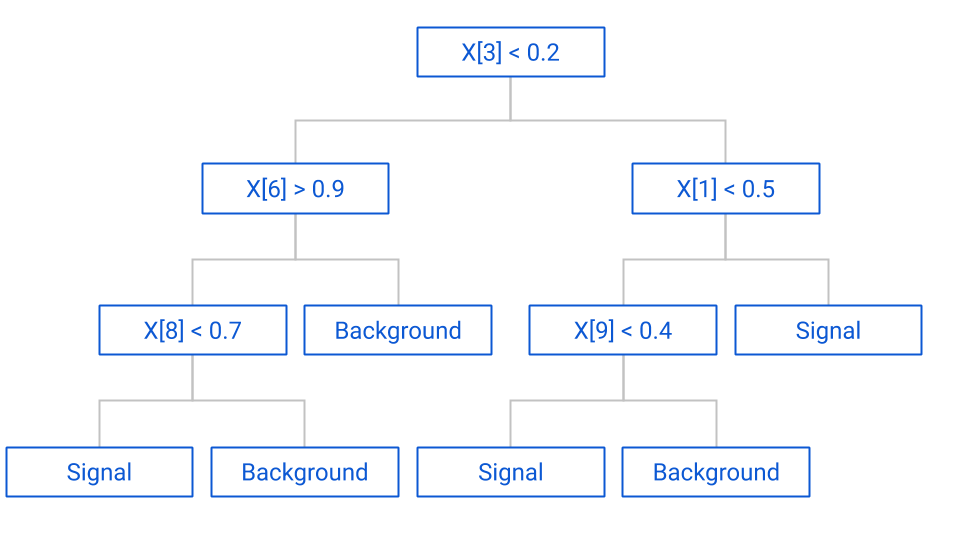
\includegraphics[width=0.8\linewidth]{Decision_tree.png}
\end{center}
\caption{\textbf{A decision tree example} To determine if a trigger is a signal or noise event the tree makes a series of cuts on the attributes x[N]. If the inequality in a node is true, then the next node is the branch to the left. Otherwise the next node is the one to the right. }
\label{fig:tree}
\end{figure}

We can improve the performance of the classifier by using an \textit{ensemble} (or \textit{forest}) of trees. This means training multiple distinct trees, and each tree independently classifies the trigger. The final classification of each trigger is a normalised sum of the outputs of each tree, with +1 corresponding to signal, and -1 corresponding to background. This leads to different regions of the parameter space having different MVA scores, as can be seen in fig.\ref{fig:mvacuts}. The higher the score, the more likely an event is to be a signal. 

\begin{figure} % Example of including images
\begin{center}
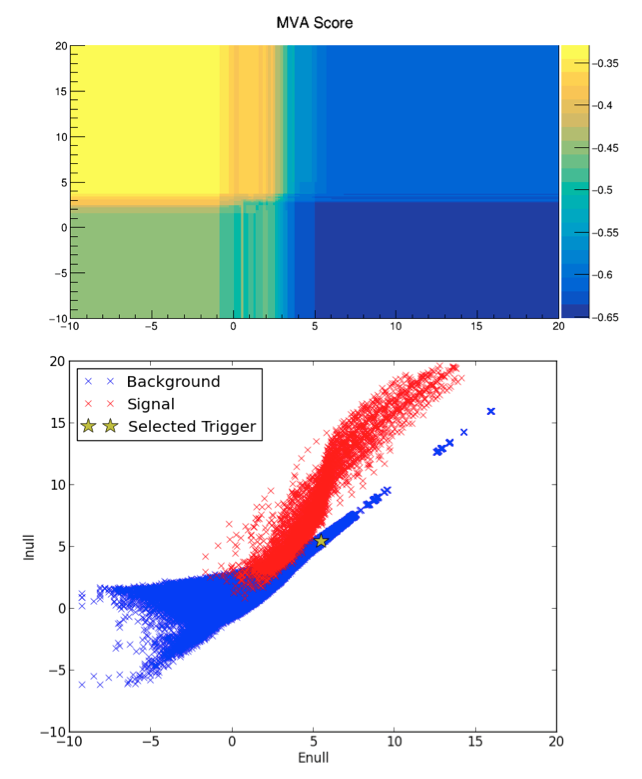
\includegraphics[width=0.8\linewidth]{mva_trigger_and_score.png}
\end{center}
\caption{\textbf{Visualising the Classifier} In the bottom plot you can see the value for log(Enull) and log(Inull) for all the signal and background training data used to build the classifier. We chose one of these events at random (indicated by the star) and varied Enull and Inull to see how it changed the MVA score, indicated by the colour in the top plot. As you can see, increasing Inull and decreasing Enull leads to the event being more likely to be classed as a signal. This is akin to the xpipeline cut shown in fig.\ref{fig:xcuts}. }
\label{fig:mvacuts}
\end{figure}


To train a decision tree, we need methods to find the variable to cut on and the position of the cut for each decision node, and the label in each leaf node that best discerns between signal and background. Each of these values is set by brute force: Trying each possible combination of cuts and labels to get the best performance on the training events. Ensemble methods work best when each classifier in the ensemble is independent of the others, so training every tree on the same events is not going to give optimal results. For this reason each tree is trained on some subset of the training set.  We could pick events at random to form these subsets, but a more powerful method is to use \textit{Adaptive Boosting}. 

When using adaptive boosting, each event in the training set is given a probability that it will be selected to train the next tree. Initially each event in the training set has the same probability of being selected. Then after each tree is trained the probability of each event being selected to train the next tree is updated such that misclassified events are more likely to be included in the training set for the next tree. The misclassifed events have their probability of being selected for training the next tree updated by the \textit{boost weight}, given by
\begin{equation}
\alpha = \frac{1 - \text{err}}{\text{err}} 
\end{equation}
where err is the misclassification rate. The weights are then renormalised. 

Note that the boost weight is greater than one for\footnote{The misclassification rate is always less than half when the labels only take two possible values as the algorithms we use are always better than chance alone.} err$< 1/2$, and that as the error gets smaller, the boost weight increases. The effect of this is that each new tree is more likely to be trained on the events that are most difficult to classify. 

The ensemble output is also changed, so that it is weighted rather than being a simple sum. If the output of the $i$th tree is given by $h_i(\textbf{x})$, with $\textbf{x}$ being the event attributes, then the ensemble output is given by
\begin{equation}
H(\textbf{x}) = \frac{1}{N}\sum_{i=0}^N \ln(\alpha_i)h_i(\textbf{x)}
\end{equation}  
where $N$ is the number of tree in the ensemble. Small values indicate background events, while large values indicate a signal. 

\subsection{Data Preprocessing}\label{data-preprocessing}
Extra data preprocessing is required for the training set. Suppose a small amplitude signal injection is added close to a large amplitude glitch in the data. This trigger will be labeled as a signal, due to the injection, but the properties of the trigger will resemble a glitch, as the glitch has a much larger amplitude than the signal injection. It is essentially a background trigger labeled as a signal. This has two affects: It reduces our ability to detect real signals by making the properties of signals harder for the algorithm to learn, and it can lead to background triggers being misclassified as a Gravitational Wave signal.  

For these reasons, it is important to make sure that signal injections do not overlap in time or frequency with background triggers. To prevent this from happening we \textit{clean} the data. This means finding all of the triggers in the data for the smallest signal injection scale. The injected waveforms are too small to be detected so all of these triggers must be background. We then increase the injection amplitude and look for triggers again. Any triggers that overlap in time or frequency with the noise triggers are then identified and removed from the from the signal set. \textbf{This description of cleaning may need to change if we change the cleaning codes.}

We must also not include injections in our signal set that are too small to be detected. If we do then we would again be including triggers labeled as signal that have the properties of a noise trigger, even if there is no glitch present. For this reason we apply a threshold on the amplitude of the signal set, so any injection below that amplitude is removed. The level of the threshold is set experimentally; If it is too low then we will increase the chance of a false positive and hurt our sensitivity to real signals, but if it is too high then we will limit the classifiers ability to detect low amplitude signals. 

We also use \textit{Generalised Clustering}. This is a change in the way Xpipeline defines a trigger. Without using generalised clustering, triggers are groups of neighbouring pixels in the time-frequency maps such as in fig.\ref{fig:tfmap}. Generalised clustering allows these pixels to be separated by a user-specified number of pixels. This can boost the signal power of long triggers, as long triggers tend to contain breaks in their time-frequency maps that causes Xpipeline to list a single long trigger as multiple short triggers. The downside to using generalised clustering is that it can cause noise triggers to be grouped together as well, boosting the power of noise. This then causes our sensitivity to short triggers to be reduced slightly. Experimenting with generalised clustering in both the standard Xpipeline analysis and the MVA analysis suggests that the benefits outweigh the costs, with an improvement of between 7\% and 50\% for long inspiral and adi waveforms at the cost of a decrease of 3\% to 9\% for short sine-gaussian waveforms.  

As XTMVA is to be used for the unmodelled search, it is also important to ensure that the search can find waveforms that are not in the training set. There are several tools that we use to achieve this. The first is to limit the amount of information the classifier is given about the waveform morphology. The classifier cannot know the precise morphology of any waveform because the only attributes that the classifier trains on is the time, peak-frequency, and various measurements of the coherent and null energy between the detectors in the network. This forces the classifier to use the coherence of the triggers to make a classification, rather than the waveform morphology. 

There is still a possibility that the classifier will become too specialised to the waveforms in the training set, as the classifier is given peak frequency data and certain waveform morphologies may have particular characteristics than become apparent from the coherent and null streams. For this reason we also trained the classifier on a variety of different waveforms. The training set included long and short waveforms, and a variety of different morphologies. Some of the signals are astrophysically motivated, such as compact binary coalescence signals, while some are artificial, such as the white noise burst.

The final tool we use to ensure the classifier is sensitive to generic waveforms is to test the classifier on waveforms that are not included in the training set. If the classifier can find waveforms not in the training set, then we can be reasonably confident that it is sensitive to generic waveforms. We also try removing certain waveforms from the training set to test the robustness of the classifier. This will lead to a drop in sensitivity for that waveform, but if the drop in sensitivity is small, then we can be confident that the classifier is robust. 

\subsection{Optimisation and Validation} \label{opt}
With any machine learning algorithm, there are \textit{hyperparameters} that must be tuned. The number of trees in the ensemble, the maximum depth of the trees, and many more hyperparameters must be chosen. We optimise the hyperparamters by repeatedly running an example analysis with different hyperparameters, trying to increase the number of injected signals we could recover from the testing set. 

Setting our hyperparameters using the testing set can cause \textit{data leakage}. Data leakage is when data from outside the training set is used to build a classifier. As we tune our classifier on the testing set, it is possible that we will implicitly tune our classifier to only work well on this training and testing set. This is very similar to overtraining discussed in section \ref{ML}. To avoid this, once we have tuned the hyperparameters on a single GRB, we test the classifier on several other GRBs. If the performance drops significantly on these other GRB analyses, then we have had data leakage and we need to retune our classifier. This process of testing on previously unused data is called \textit{validation}. If there is evidence of data leakage, then we must retune our classifier and validate it again, this time using a different (previously unused) GRB so as to avoid data leakage from the validation GRB. 

Optimisation is a somewhat cyclical process, as once we have changed one hyperparameter, we must then go back and test that other parameters do not now need changing. But optimisation is not pure guess work, and in the rest of this section we will see the strategy we used to optimise our classifier. We first discuss optimising the training data to use. As mentioned in section \ref{data-preprocessing}, there are several choices to make regarding what data is used for training, such as setting the amplitude threshold. We then discuss optimising the BDT classifier itself. 

\subsubsection{Training Set}
Many of the hyperparameters mentioned in section \ref{data-preprocessing} had to be optimised. Consider the amplitude threshold applied to triggers before they are included in the training set. If this is too low then noise triggers contaminate the signal training set, but if it is too high then we limit the sensitivity of our classifier to only higher amplitude waveforms. 

We also optimised the waveforms that are included in the training set, whether to use cleaning or not, and whether to use generalised clustering. \textbf{Write more on this once we've done it.}



\begin{itemize}
\item Had to optimise the threshold as well
\item Training waveforms
\item cleaning or not
\item Gen clustering or not
\item off source injections
\end{itemize}

\subsubsection{BDT Parameters}
There are many hyperparameters that need to be set for a BDT analysis. In this section we discuss some of these hyparameters and the method we used to optimise them for our analysis. 

We began by setting values for \textit{NTrees}, the number of trees in the ensemble, and the learning rate, discussed in section \ref{bdt}. These two parameters are set first to ensure the machine learning algorithm will converge in a reasonable amount of time. Setting the learning rate  too low causes the classifier to take longer to converge. Setting the learning rate too high can cause the classifier to never converge. Similarly, using too many trees takes too long for the classifier to finish training, but too few and the training will terminate before the algorithm has converged. Setting these first ensures that we have a classifier that gives sensible results in a reasonable amount of time. While optimising, we set these values slightly high, to ensure that our classifier converges and does so quickly while we optimise our other parameters. Once the other parameters are set, we again optimise NTrees and the learning rate, increasing the number of trees and decreasing the learning rate to ensure the algorithm reaches its optimum performance, even if it increases the time taken for training.

We now tune the tree-specific parameters. Unlike the number of trees and the learning rate which are primarily tuned to ensure the classifier will converge in a reasonable time, these parameters are set to ensure that the classifier is accurate but does not overtrain. Overtraining can happen when the trees are allowed to make cuts that are too fine, carving out regions of parameter-space around anomalous events in the training set rather than finding cuts that generalise beyond the training data. The way to prevent this is to limit how fine the cuts made by the decision trees are allowed to be, while allowing cuts that are fine enough to pick out the general features of signal and background events in our data. There are several hyperparameters we can set to do this, which must all be tuned. 

The first of these is the maximum depth of the trees, which is the maximum number of cuts a tree can make before it reaches a leaf node. Each cut divides the parameter-space into ever smaller regions which it labels as background or signal. Setting the maximum number of cuts too low will therefore cause the classifier to be too coarse in dividing up the parameter-space, resulting in poor accuracy. Increasing the maximum depth allows the classifier to pick out smaller features in the parameter-space. If the maximum depth is too high then the classifier will overtrain; dividing the parameter-space into precisely the regions that work for the training set and losing generality. As we are using adaptive boosting, it is recommended \textbf{cite TMVA userguide} to use trees with fewer cuts. For this reason we tried values from 2-16, finding that for our problem a maximum depth of 8 was optimal. 

A related hyperparameter is the minimum number of events that we allow in a leaf node. If we allow the training algorithm to have any number of events in a leaf node, then it will occasionally find cuts that results in a small number of events in one or more of the leaf nodes. The again allows for the carving out of anomalous events in the training set rather than finding cuts that can generalise beyond the training set. Conversely, setting the minimum number of events allowed in the leaf nodes to be too high does not allow the classifier to pick out the key features in the data. We used a grid search over the values 100-1600 for the minimum number of events per leaf node and found the optimal value to be 400. 

The final hyperparameter we set is the number of cuts that the training algorithm scans over to find the best cut. When the classifier is training it searches for the best way to cut the parameter-space into a signal subspace and a background subspace. To do this we can try every possible cut on every parameter. This can be very slow and lead to overtraining. To speed up our analysis and reduce the chance of overtraining, we can choose the number of cuts to try on each parameter. For example, we may decide to use 10 cuts for each parameter. In this case the algorithm will tune the cut on a parameter which ranges from 0-100 by trying cuts at 0,10,20,... and selecting the best of these cuts. To tune the number of cuts we wanted to use, we tried values from 10-160 as well as allowing the classifier to try every possible cut. We found that 80 cuts was optimal for our purposes. 

\begin{itemize}
\item This can definitely be phrased better
\end{itemize}

\subsubsection{Result of Optimisation}

\begin{figure} % Example of including images
\begin{center}
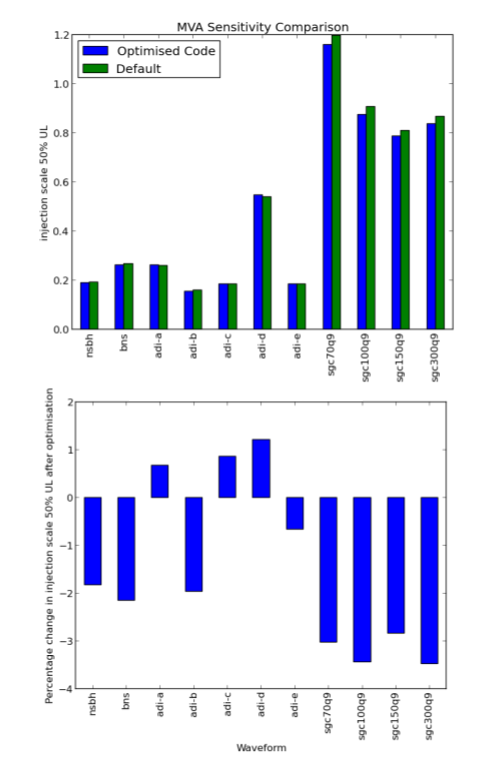
\includegraphics[width=0.8\linewidth]{opt_comparison.png}
\end{center}
\caption{\textbf{Effect of Optimisation.} Used GRB E264930  }
\label{fig:opt compare}
\end{figure}

\section{Effectiveness of XTMVA}
\subsection{Comparison to Xpipeline}
\begin{itemize}
\item Change in sensitivity
\item Table of results
\item Speed improvement (real time and cpu time)
\end{itemize}


\begin{figure} % Example of including images
\begin{center}
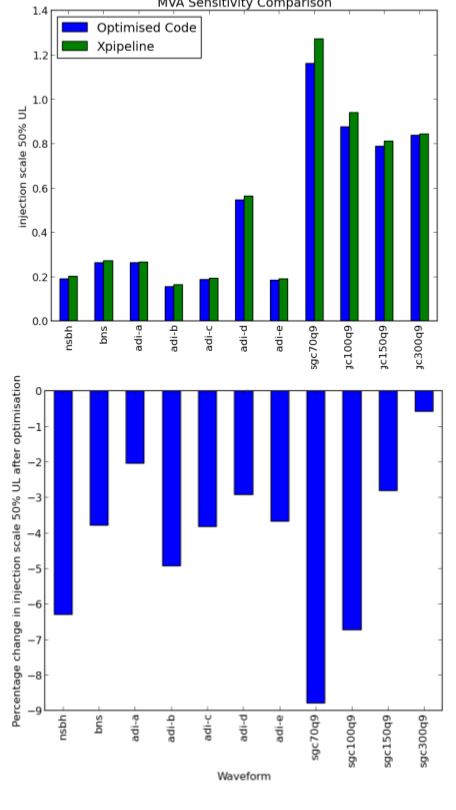
\includegraphics[width=0.8\linewidth]{x_compare.png}
\end{center}
\caption{\textbf{MVA Improvement.} Used GRB E264930  }
\label{fig:x compare}
\end{figure}

\subsection{Unsolved Problems}
\begin{itemize}
\item Unstable
\item Issue of data leakage
\item Ineffectiveness of optimisation
\item Still having issues with long waveforms
\end{itemize}

\subsection{Future Work}
\begin{itemize}
\item Machine learning such as this shows promise
\item Compare to other GW machine learning searches
\item Limited scope of the pipeline is probably beneficial
\item New machine learning software available now that is more transparent
\item Get working with generalised clustering and long inj but still with off source injections
\end{itemize}


\appendix
\appendixpage
\addappheadtotoc
\section{General Relativity}

Christoffel Symbol
\begin{equation} \label{christ}
\Gamma^\lambda\mn=\frac{1}{2}g^{\lambda \rho} [\partial_\nu g_{\mu \rho} + \partial_\mu g_{\nu \rho}-\partial_\rho g\mn]
\end{equation}
Riemann Curvature Tensor  
\begin{equation} \label{rct}
R^\mu_{\lambda \alpha \beta} = \partial_\alpha \Gamma^\mu_{\lambda \beta} -\partial_\beta \Gamma^\mu_{\lambda \alpha} + \Gamma^\mu_{\nu \alpha} \Gamma^\nu_{\lambda \beta} - \Gamma^\mu_{\nu \beta} \Gamma^\nu_{\lambda \alpha}
\end{equation}
Ricci Tensor
\begin{equation} \label{rt}
R\mn=g^{\alpha \beta} R_{\alpha \mu \beta \nu}=R^\beta_{\mu \beta \nu}
\end{equation}
Ricci Scalar
\begin{equation} \label{rs}
R=g^{\alpha \beta}R_{\alpha \beta}=R^\beta_\beta
\end{equation}
The Einstein Equations
\begin{equation} \label{eineq}
G\mn =R\mn -\frac{1}{2} R g\mn=\frac{8 \pi G}{c^4}T\mn
\end{equation}
Alternative form of the Einstein equations
\begin{equation} \label{alt einstein}
R\mn = \frac{8 \pi G}{c^4}\left( T\mn - \frac{1}{2}Tg\mn \right) 
\end{equation}
% ----------------------------
% postamble 

\backmatter
% add bibligography

\end{document}
